\documentclass{book}
\usepackage[spanish]{babel}  % Add the babel package with Spanish language option
\usepackage{amsmath}  % Include the amsmath package
\usepackage{graphicx}  % Include the graphicx package
\usepackage{float}     % Include the float package
\usepackage{array}
\usepackage{pgfplots}
\usepackage{subcaption}
\usepackage[export]{adjustbox}
\usepackage{pst-plot}
\usepackage{amssymb}
\usepackage{siunitx}
\usepackage{esint}
\usepackage[dvipsnames]{xcolor}
\usepackage{circuitikz}
\usepackage{tikz}
\usetikzlibrary{babel}
\usepackage{mathtools}

\usepackage[left=3cm,top=3cm,right=3cm,bottom=3cm]{geometry}

\title{Mecánica de fluidos}
\author{Bogurad Barañski Barañska \and Adrián Teixeira de Uña}

\date{\today}

\begin{document}
	\maketitle
	\frontmatter
		
		\tableofcontents % Insert a table of contents
		\addcontentsline{toc}{chapter}{Índice general}
	
	\mainmatter
		
\section{Tema 1: Introducción y generalidades sobre metrología}
\subsection{Definiciones}
\begin{enumerate}
	\item \underline{\textbf{Magnitud}}: 
	\item \underline{\textbf{Magnitud básica}}:
	\item \underline{\textbf{Magnitud derivada}}:
	\item \underline{\textbf{Unidad de medida}}:
	\item \underline{\textbf{Unidad coherente}}:
	\item \underline{\textbf{Sistema de unidades}}:
	\item \underline{\textbf{Valor de una magnitud}}:
	\item \underline{\textbf{Valor verdadero}}:
	\item \underline{\textbf{Valor convencionalmente verdadero}}:
	\item \underline{\textbf{Medida}}:
	\item \underline{\textbf{Medición general}}:
	\item \underline{\textbf{Medición metrológica}}:
	\item \underline{\textbf{Mensurando}}:
	\item \underline{\textbf{Magnitud de influencia}}:
	\item \underline{\textbf{Señal de medida}}:
	\item \underline{\textbf{Instrumento de medida}}:
	\item \underline{\textbf{Cadena de medida}}:
	\item \underline{\textbf{Valor nominal}}:
	\item \underline{\textbf{Campo de medida}}:
	\item \underline{\textbf{Rango de medida}}:
	\item \underline{\textbf{Constante de medida}}:
	\item \underline{\textbf{Estabilidad}}:
	\item \underline{\textbf{Transparencia}}:
	\item \underline{\textbf{Deriva}}:
	\item \underline{\textbf{Zona muerta}}:
	\item \underline{\textbf{Sensibilidad}}:
	\item \underline{\textbf{Resolución}}:
	\item \underline{\textbf{Veracidad}}:
	\item \underline{\textbf{Precisión}}:
	\item \underline{\textbf{Exactitud}}:
	\item \underline{\textbf{Sesgo}}:
	\item \underline{\textbf{Linealidad}}:
	\item \underline{\textbf{Índice de clase}}:
	\item \underline{\textbf{Incertidumbre de medida}}:
	\item \underline{\textbf{Error de medida }}:
	\item \underline{\textbf{Error aleatorio}}:
	\item \underline{\textbf{Error sistemático}}:
	\item \underline{\textbf{Tolerancia}}:
	\item \underline{\textbf{Incertidumbre}}:
\end{enumerate}
\subsection{Causas de errores}
\subsection{Ley propagación de incertidumbres}
\subsection{Estimación de la incertidumbre}
\subsection{Relación tolerancia incertidumbre}
\subsection{Relación incertidumbre resolución}
		\chapter{Energía eléctrica y desarrollo sostenible.}

\section{Introducción al desarrollo sostenible.}
El desarrollo nació en los años 70 en los países nórdicos y se define como:
\begin{itemize}
	\item [-] El que satisface
	nuestras necesidades actuales sin poner en peligro la
	capacidad de las generaciones futuras para satisfacer sus
	propias necesidades abarcando:
	\begin{itemize}
		\item El capital social
		\item El capital ambiental
		\item El capital económico
	\end{itemize}
\end{itemize}
\subsection{Cumbres climáticas.}
\begin{itemize}
	\item [-] \textbf{Rio de Janeiro (1992):}
		Se crea la Comisión del Desarrollo Sostenible para impulsar la sostenibilidad de las políticas de desarrollo humano y gestionar sus riesgos.
	\item [-] \textbf{Cumbre del Protocolo de Kyoto (1997):}
		Se adquiere un compromiso entre los países industrializados con el \textbf{objetivo} de reducir las emisiones de gases de efecto invernadero un 5,9\% en el periodo 2008 - 2012 con respecto a 1990 (año base). En una fase inicial no incluía a países en desarrollo como China e India por su baja contaminación per capita.
	\item [-] \textbf{Cumbre de París (2015):}
		Se comprometen los países a que la temperatura mundial no aumente más de 2\textdegree C respecto a los niveles preindustriales y limitarlo a 1,5\textdegree C para el 2020.
	\item [-] \textbf{Cumbre de Marrakech (2016):}
		Se ratifican los acuerdos de la Cumbre de París y se compromete reducir el 80\% de las emisiones de CO$_2$ para 2050.
	\item [-] \textbf{Cumbre de Katowice (2018):}
		Limitar a un incremento a final de siglo de 1,5 a 2\textdegree C respecto a los niveles preindustriales.
	\item [-] \textbf{Cumbre de Chile celebrada en Madrid (2019):}
		Los grandes contaminadores se niegan a intensificar los esfuerzos para mantener la temperatura por debajo de 1,5\textdegree C.
	\item [-] \textbf{Cumbre de Glasgow (2021):}
		Se mantiene el objetivo de 1,5\textdegree C para 2030. Acuerdo China - USA para reducir las emisiones de metano. Compromiso de 130 países para poner fin a la deforestación.
	\item [-] \textbf{Cumbre de Sharm el-Sheij en Egipto (2022):}
		Se acuerdan:
		\begin{itemize}
			\item Una alianza global contra la sequía.
			\item Una coalición contra la deforestación.
			\item Impulsar el hidrógeno verde.
			\item Impulsar la energía eólica marina.
		\end{itemize}
	\item [-] \textbf{Cumbre de Dubai(2021):}
		Se acuerda reducir las emisiones mundiales de gases de efecto invernadero un 43\% hasta
		2030 y un 60\% hasta 2035 en relación con los niveles de 2019, y emisiones netas de dióxido de carbono cero
		para 2050.
\end{itemize}
\section{Gases de efecto invernadero.}
\subsection{CO$_2$ equivalente.}
Es una forma de poder reducir el impacto climático a una unidad común y así, poder compararlos. Para calcularlo se emplea el valor \textbf{GWP} (Global Warming Potencial) o \textbf{PCG} (Potencial de calentamiento global) que miden cuanto calor atrapan en comparación con el CO$_2$ para un periodo de tiempo. 


Este valor depende de:
\begin{itemize}
	\item [-] La absorción de radiación infrarroja.
	\item [-] La ubicación del espectro de absorción.
\end{itemize}
\subsection{Dióxido de carbono (CO$_2$).}
Es la sustancia que más contribuye al efecto invernadero. Absorbe gran parte de la radiación solar incidente.
\subsection{Óxido nitroso (N$_2$O) y óxidos de nitrógeno (NO$_x$ ).}
Son los gases de efecto invernadero más destructivos con la capa de ozono. Relacionados con el sector agrario y la quema de combustible.
\subsection{Metano (CH$_4$).}
Tiene un potencial de calentamiento muy elevado GWP = 25. Se emite por el sector ganadero, el de tratamiento de residuos y durante el transporte de hidrocarburos.
\subsection{Hidrofluorocarbonos (HFC).}
Son gases empleados como refrigerantes. No dañan al ozono pero tienen un GWP = 1000 y una larga permanencia en la atmósfera.
\subsection{Perfluororcarburos (PFC).}
Similares a los HFC.
\subsection{Hexafluoruro de azufre (SF$_6$).}
Se emplea para equipos de distribución de energía eléctrica. Tiene propiedades similares a los HFC y PFC.

\begin{table}[H]
	\centering
	\begin{tabular}{p{2cm}p{2cm}p{2cm}p{2cm}p{2cm}}
		\hline
		\textbf{ } & \textbf{CO$_2$} & \textbf{ClFCs} & \textbf{CH$_4$} & \textbf{N$_2$O} \\ \hline
		Importancia según contribución al efecto invernadero & Más del 50\% & 20 \% aprox. & 12 a 14 \% & 6 a 7 \% \\ \hline
		Tiempo de permanencia en la atmósfera & 50 - 200 años & 75 - 100 años & 7 a 10 años & 150 años aprox. \\ \hline
		Tasa de crecimiento anual (\%)&0,5&4-5&1&0,35\\ \hline 
		Principal origen de la contaminación&Combustión del petróleo, carbón y gas deforestación&Aerosoles y disolventes Espumas industriales Equipos de refrigeración&Pantanos Ganadería Minería&Fertilizantes Combustible fósiles\\ \hline 
	\end{tabular}
	\label{tab:my-table}
\end{table}

\section{Efecto invernadero.}
Como consecuencia de los gases de efecto invernadero se absorbe una mayor cantidad de radiación infrarroja que escaparía de la tierra y, por tanto, aumentando la temperatura atmosférica. 
\begin{figure}[H]
	\centering
	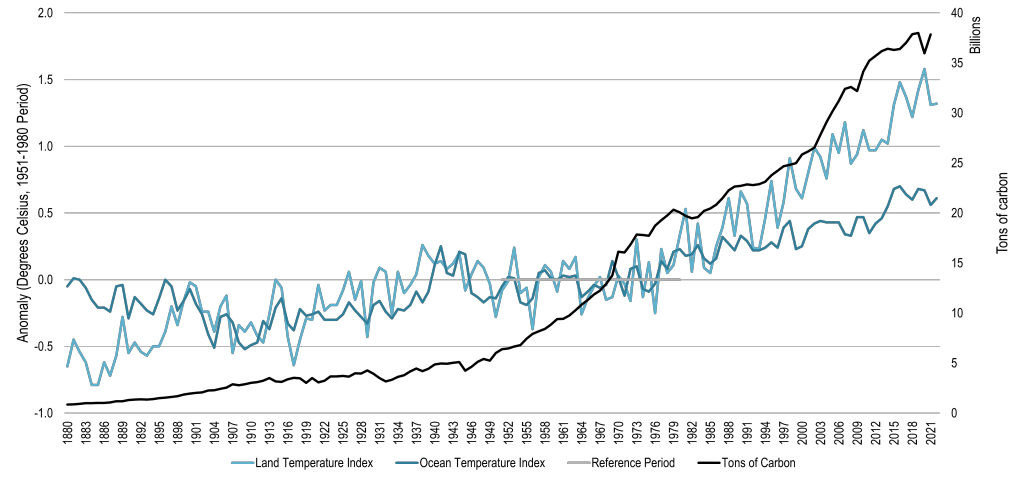
\includegraphics[width=0.7\linewidth]{res/tema2/T-Emisiones}
	\label{fig:t-emisiones}
\end{figure}
\subsection{Forzamiento radiactivo o climático.}
Es la diferencia entre la radiación solar absorbida por la Tierra y la energía irradiada de vuelta al espacio. Esta diferencia se contempla mediante el RCP donde:
\begin{itemize}
	\item [-] RCP = 2 es un escenario con el indicador muy bajo.
	\item [-] RCP = 8,5 es un escenario con el indicador muy alto.
\end{itemize}

\begin{table}[h]
	\centering
	\renewcommand{\arraystretch}{1.5}
	\begin{tabular}{cccccc}
		\hline
		Escenario & Forz. Radiat. (W/m\textsuperscript{2} en 2100) & \multicolumn{2}{c}{GC} & \multicolumn{2}{c}{GtCO$_2$} \\
		\cline{3-6}
		& &Media & Rango & Media & Rango \\
		\hline
		RCP2.6 & 2.8 & 270 & 140 a 410 & 990 & 510 a 1505 \\
		RCP4.5 & 4.5 & 780 & 595 a 1005 & 2880 & 2180 a 3690 \\
		RCP6.0 & 6 & 1060 & 840 a 1250 & 3885 & 3080 a 4585 \\
		RCP8.5 & 8.5 & 1685 & 1415 a 1910 & 6180 & 5163 a 7005 \\
		\hline 
	\end{tabular}
\end{table}

\begin{table}[H]
	\centering
	\renewcommand{\arraystretch}{1.5}
	\begin{tabular}{p{4cm}p{2cm}p{1cm}p{3cm}p{1cm}p{3cm}}
		\hline
		& \textbf{Escenario} &
		\multicolumn{2}{c}{\textbf{2046-2065}}  & \multicolumn{2}{c}{\textbf{2081-2100}} \\ 
	
		& &\textbf{Media} & \textbf{Rango probable} & \textbf{Media} &\textbf{Rango probable} \\ 
		\hline
		Cambio en la   & 
		RCP2,6 & 1 & 0,4 a 1,6 &1 &0,3 a 1,7\\
		temperatura media global&RCP4,5 & 1,4 & 0,9 a 2,0 &1,8 & 1,1 a 2,2 \\
		del aire en superficie & RCP6 & 1,3 & 0,8 a 1,8 & 2,2 & 1,4 a 3,1\\
		(en °C)& RCP8,5 & 2 & 1,4 a 2,6 & 3,7 & 2,6 a 4,8 \\
		\hline
		Elevación media mundial   & RCP2,6 & 0,24 & 0,17 a 0,32 & 0,4  & 0,26 a 0,55 \\
		del nivel del mar& RCP4,5 & 0,26 & 0.19 a 0,33 & 0,47 & 0,32 a 0,63 \\
		(en metros)& RCP6   & 0,25 & 0.18 a 0,32 & 0,48 & 0,33 a 0,63 \\
		& RCP8,5 & 0,3  & 0,22 a 0,38 & 0,63 & 0,45 a 0,82 \\
		\hline
	\end{tabular}
\end{table}
\newpage
\subsection{Evolución de las emisiones de CO$_2$ equivalente en España.}
España se comprometió con la unión europea en reducir emisiones para el periodo 2008 - 2012 en un 15\% respecto a 1990 (Fase I y II). Para el periodo 2013 - 2020 se comprometió a reducir emisiones en un 20\% respecto a los niveles del año base.
 
\begin{figure}[H]
	\centering
	\begin{tikzpicture}
		\begin{axis}[
			xlabel={Año},
			ylabel={kt CO\textsubscript{2}},
			xtick={1990,1995,2000,2005,2010,2015,2020,2025},
			ytick={270, 300, ..., 450},
			grid=both,
			grid style={line width=.1pt, draw=gray!10},
			major grid style={line width=.2pt,draw=gray!50},
			width=12cm,
			height=8cm,
			]
			\addplot[mark=*] coordinates {
				(1990, 287.710)
				(1995, 327.011)
				(2000, 383.276)
				(2005, 438.760)
				(2010, 354.652)
				(2015, 333.623)
				(2018, 328.905)
				(2019, 309.814)
				(2020, 272.244)
				(2021, 288.848)
				(2022, 314.000)
			};
		\end{axis}
	\end{tikzpicture}

\end{figure}

En cuanto a las emisiones asociadas a la generación eléctrica:
\begin{table}[H]
	\centering
	\begin{tabular}{p{3cm}l*{11}{c}}
		\toprule
		tCO\textsubscript{2} $\times$ 1.000.000& 2011 & 2012 & 2013 & 2014 & 2015 & 2016 & 2017 & 2018 & 2019 & 2020 & 2021 & 2022 \\
		\midrule
		Carbón &   41,0 & 51,1 & 37,5 & 41,1 & 50,0 & 35,4 & 42,8 & 36,0 & 12,4 & 4,9 & 4,9 & 7,5 \\
		Fuel + Gas  &  0,0 & 0,0 & 0,0 & 0,0 & 0,0 & 0,0 & 0,0 & 0,0 & 0,0 & 0,0 & 0,0 & 0,0 \\
		Motores diésel &  2,9 & 2,9 & 2,7 & 2,6 & 2,7 & 2,8 & 2,7 & 2,2 & 2,0 & 1,6 & 1,7 & 1,7 \\
		Turbina de gas &  0,9 & 1,0 & 0,7 & 0,8 & 0,7 & 0,5 & 0,7 & 1,0 & 0,7 & 0,4 & 0,5 & 0,7 \\
		Turbina de vapor &  2,3 & 2,4 & 2,2 & 1,8 & 2,0 & 2,3 & 2,4 & 2,2 & 2,0 & 1,3 & 1,0 & 1,1 \\
		Ciclo combinado  & 21,0 & 16,4 & 11,4 & 10,5 & 12,0 & 12,0 & 14,9 & 11,8 & 21,2 & 17,1 & 17,4 & 26,2 \\
		Cogeneración  &  11,6 & 12,3 & 11,7 & 9,2 & 9,6 & 9,8 & 10,7 & 11,0 & 11,3 & 10,1 & 9,7 & 6,6 \\
		Residuos no renovables &  0,3 & 0,4 & 0,4 & 0,5 & 0,6 & 0,6 & 0,6 & 0,6 & 0,5 & 0,7 & 0,8 & 0,6 \\
		Total Emisiones &  80,1 & 86,4 & 66,6 & 66,5 & 77,6 & 63,5 & 74,9 & 64,9 & 50,0 & 36,1 & 35,9 & 44,4 \\ 
		\\
		\hline
		\\
		Factor de emision de CO\textsubscript{2} (tCO\textsubscript{2}/MWh) &  0,29 & 0,31 & 0,24 & 0,25 & 0,29 & 0,24 & 0,29 & 0,25 & 0,19 & 0,15 & 0,14 & 0,16 \\
		\bottomrule
	\end{tabular}
\end{table}

En cuanto a los rendimientos de diversas plantas de generación eléctrica:
\begin{table}[h]
	\label{tab:conversion-efficiency}
	\begin{tabular}{lcccc}
		\toprule
		&Eficiencia conversión&\multicolumn{3}{c}{Emisiones en gramos/kWh} \\
		\cline{3-5}
		&  (\%) & NOx & SO2 & CO2 \\
		\midrule
		Carbón pulverizado (sin descontaminar S) & 36 & 1.29 & 17.2 & 884 \\
		Carbón pulverizado (con descontaminación S) & 36 & 1.29 & 0.86 & 884 \\
		Carbón en lecho fluidificado & 37 & 0.42 & 0.84 & 861 \\
		Ciclo combinado de carbón gasificado & 42 & 0.11 & 0.3 & 758 \\
		Turbina de gas & 39 & 0.23 & 0 & 470 \\
		Ciclo combinado de turbina de gas & 53 & 0.1 & 0 & 345 \\
		\bottomrule
	\end{tabular}
\end{table}
\newpage
\section{Protocolo de Kioto.}
El Protocolo de Kioto estableció 3 vías para su cumplimiento:
\subsection{Políticas y medidas.}
Directiva 2033/87 CE de Comercio de Derechos de Emisión de gases
de efecto invernadero en la Unión Europea.
\subsection{Creación de sumideros.}
Se consideran sumideros todos los sistemas por los que se extraen gases de la atmósfera. Se consideran sumideros actividades como la reforestación.
\subsection{Mecanismos flexibles.}
\begin{enumerate}
	\item \textbf{Comercio de derechos de emisión (CDE):}
		Establece una asignación de una determinada cantidad de derechos de emisión gratuitos para
		las centrales térmicas y el sector industrial que equivalen a 1 tonelada de CO$_2$. Un país que haya conseguido reducir sus emisiones podrá vender a otro país que no llegue a su objetivo previsto. En España se llama \textbf{PNA} (Plan Nacional de Asignación).
	\item \textbf{Mecnismo de desarrollo limpio (MDL):}
		El país desarrollado invierte en tecnologías limpias en países en vías de desarrollo.
	\item \textbf{Aplicación conjunta (AC):}
		Un país desarrollado invierte en otro país desarrollado en un proyecto de energía limpia.
\end{enumerate}
\section{PNA.}
	La Directiva de la Unión Europea sobre Comercio de Emisiones (2003/87/CE) establece que cada Estado
	miembro deberá elaborar un Plan Nacional de Asignación (PNA) en el que se determinen la cantidad total de
	derechos a asignar durante un periodo y el procedimiento de asignación aplicado.
	
	
	Actualmente en España se asigna mediante el PNA IV donde se permiten unas emisiones de CO$_2$ = 44 MtCO$_{2-eq}$
\section{Precio de emisión.}
SENDECO2 es la plataforma que proporciona a todos los empresarios un lugar donde intercambiar Derechos de Emisión (EUAs) por Créditos de carbono (CERs) que certifican que se deja de emitir una tonelada de CO$_2$.
\subsection{Evolución del precio del derecho de emisión.}
\begin{figure}[H]
	\centering
	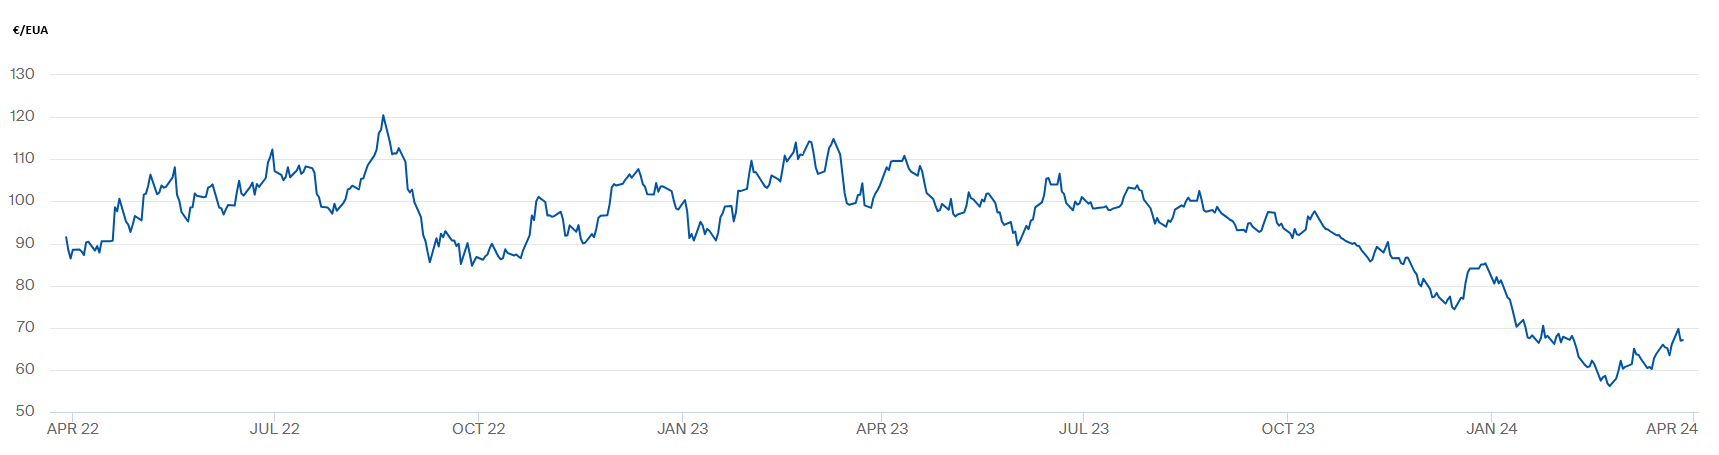
\includegraphics[width=1\linewidth]{res/tema2/precioEUA}
	\label{fig:t-emisiones}
\end{figure}
\newpage
\subsection{Influencia coste de emisión en el mercado eléctrico.}
Desde el año 2021 las centrales térmicas no tienen cantidades asignadas gratuitas y por ello, tienen que comprar derechos de emisión. Este coste repercute en el coste de la generación ofertado y, por tanto el precio de la energía como se puede ver en la figura inferior.
\begin{figure}[H]
	\centering
	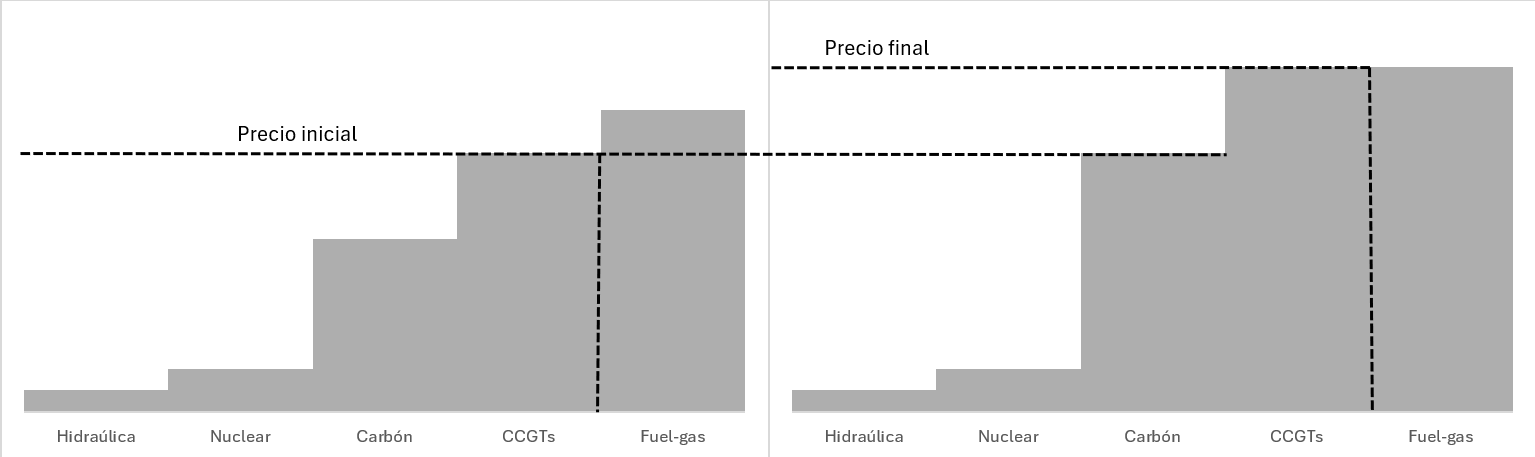
\includegraphics[width=1.2\linewidth]{res/tema2/variacionPrecio}
	\label{fig:variacionprecio}
\end{figure}
\subsection{Factor de emisión.}
El factor de emisión (fe) representa la cantidad de CO$_2$ que se genera por MWh de electricidad producida en bornes de la central:
\[fe=\frac{tCO_{2-eq}}{MWhe}=\frac{tCO_{2-eq}}{TJ}\]
Los factores de emisión se actualizan anualmente.
\subsection{Cálculo del factor de emisión.}
Para el cálculo se emplea la siguiente expresión:
\[f\left(\frac{tCO_2}{MWh}\right)=\frac{tCO_2}{TJ}\cdot\frac{3,6 TJ}{1000 MWh}\cdot\frac{100}{\eta}\]
\begin{enumerate}
	\item \textbf{Centrales térmicas de carbón:}
		El carbón es un combustible con un alto contenido en carbono y por ello genera una cantidad elevada de CO$_2$ por MWhe. El tep (tonelada equivalente petróleo) es una unidad para referir la energía con respecto a la obtenida con una tonelada de petróleo.
	\begin{table}[H]
		\centering
		\renewcommand{\arraystretch}{1.1}
		\begin{tabular}{cm{2cm}m{2cm}m{3cm}m{2cm}m{2cm}}
			\hline
			\textbf{Combustible} & \textbf{ktCO2/ktep} & \textbf{TJ/ktep} & \textbf{Factor de Emisión  combustible (tCO2/TJ)} & \textbf{Rendimiento eléctrico (\%)} & (tCO2/MWh)\\  
			\hline
			Hulla + Antracita nacional & 4,032 & 41,868 & 96,303 & 36\% & 0,96 \\
			Carbón importado           & 4,032 & 41,868 & 96,303 & 36\% & 0,96 \\
			Lignito negro              & 3,861 & 41,868 & 92,218 & 36\% & 0,92 \\
			Lignito pardo              & 3,983 & 41,868 & 95,132 & 36\% &0,95 \\ \hline
		\end{tabular}
	\end{table}
	
	\item \textbf{Centrales térmicas de ciclo combinado con gas natural:}
		Utilizan gas natural, un combustible con menor contenido en carbono que junto a su elevado rendimiento hace que tenga un menor factor de emisión.
		\begin{table}[H]
		\centering
		\renewcommand{\arraystretch}{1.1}
		\begin{tabular}{cm{2cm}m{2cm}m{3cm}m{2cm}m{2cm}}
			\hline
			\textbf{Combustible} & \textbf{ktCO2/ktep} & \textbf{TJ/ktep} & \textbf{Factor de Emisión  combustible (tCO2/TJ)} & \textbf{Rendimiento eléctrico (\%)} & (tCO2/MWh)\\  
			\hline
			Gas natural & 2,337 & 41,868 & 55,818 & 54\% & 0,37 \\
		 \hline
		\end{tabular}
	\end{table}
	\newpage
	\item \textbf{Centrales térmicas de fuel-gas:}
		Debido a su heterogeneidad se utilizan valores medios empíricos para este conjunto de centrales.
				\begin{table}[H]
			\centering
			\renewcommand{\arraystretch}{1.1}
			\begin{tabular}{cm{2cm}}
				\hline
				\textbf{Combustible}  & (tCO2/MWh)\\  
				\hline
				Gas natural & 0,77 \\
				\hline
			\end{tabular}
		\end{table}
	\item \textbf{Centrales hidráulicas, renovables y nuclear:}
		No emiten CO$_2$ para generar electricidad.
		\begin{table}[H]
			\centering
			\renewcommand{\arraystretch}{1.1}
			\begin{tabular}{cm{2cm}}
				\hline
				\textbf{Combustible}  & (tCO2/MWh)\\  
				\hline
				Centrales hidráulicas, renovables y nuclear & 0
				 \\
				\hline
			\end{tabular}
		\end{table}
	\item \textbf{Cogeneración:}
		Consiste en la producción combinada de calor y electricidad, lo que permite conseguir un rendimiento conjunto superior.
		\begin{table}[H]
			\centering
			\renewcommand{\arraystretch}{1.1}
			\begin{tabular}{cm{2cm}}
				\hline
				\textbf{Combustible}  & (tCO2/MWh)\\  
				\hline
				Cogeneración & 0,37
				\\
				\hline
			\end{tabular}
		\end{table}
	\item \textbf{Residuos:}
		Como existe una gran heterogeneidad en los combustibles empleados se toma un valor medio. En el caso de la biomasa su factor de emisión es nulo porque son neutros a nivel de emisiones. Además las emisiones de N$_2$O asociadas a los residuos no son significativas a nivel de cálculos del factor de emisión.
		\begin{table}[H]
			\centering
			\renewcommand{\arraystretch}{1.1}
			\begin{tabular}{cm{2cm}m{2cm}}
				\hline
				\textbf{Combustible} & \textbf{Rendimiento eléctrico (\%)} & (tCO2/MWh)\\  
				\hline
				Residuos &25\%& 0,24
				\\
					Biomasa &-& 0
				\\
				\hline
			\end{tabular}
		\end{table}
\end{enumerate}
\subsection{Emisiones en la combustión.}
Las fuentes de combustión que producen emisiones de CO$_2$ se calculan multiplicando el contenido de energía por un factor de emisión y oxidación (se asume igual a 1 el factor de oxidación).
\[\text{Emisiones CO}_2 = \text{Datos de la actividad} \times \text{Factor de emisión} \times \text{Factor de oxidación}\]

Los datos de actividad se expresan como el contenido de energía neto del combustible consumido [TJ] durante un periodo.
\[\text{Contenido de energía [TJ]}=\text{Combustible consumido [t o m$^3$]}\times \text{Poder calorífico combustible [TJ/t o TJ/m$^3$]}\]

El poder calorífico neto es un valor representativo de la energía liberada en la combustión en forma de calor. Esta magnitud tiene límite superior (PCS) e inferior (PCI) en función de la humedad del combustible.

\[[PCI]_s (kcal/kg)=[PCS]_s-597\cdot (9H+H_2O)\]
\begin{itemize}
	\item [-] H $\rightarrow$ \% de hidrógeno contenido en el combustible (base seca).
	\item [-] H$_2$O $\rightarrow$ \% de humedad del combustible.
\end{itemize}

\subsection{Emisiones evitadas con las energías renovables.}
Las energías renovables en España permitieron reducir la emisión de 55,6 millones de tCO$_2$ y cubrieron el 42,2\% de la demanda eléctrica.
\newpage
\section{Combustibles fósiles.}
\subsection{Combustible sólidos.}
\begin{enumerate}
	\item \textbf{Biomasa:}
		El combustible esta compuesto de materia vegetal que había sido creada a través de la fotosíntesis:
		\[6 CO_2 + 6 H_2O + 112 kcal/mol \rightarrow C_6 (H_2O)_6 + 6 O_2 ( Glucosa)\]
		Por tanto, la fotosíntesis fija al año 18.000 Mt de CO$_2$ y por tanto, quemar esta planta no produce más CO$_2$ que el que liberaría al morir por fermentación. De esta manera, se podría considerar renovable.
	\item \textbf{Carbón:}
		Es una roca de fácil combustión con aproximadamente el 50\% del peso en carbono. No obstante, en función del porcentaje de carbono cambia el poder calorífico:
		\begin{table}[H]
			\centering
			\renewcommand{\arraystretch}{1.1}
			\begin{tabular}{cccc}
				\hline
				&\textbf{Lignito} & \textbf{Hulla} & \textbf{Antracita}\\  
				\hline
			Densidad &  1,1-1,3&1,2-1,5  &1,4-1,8\\ 
			Humedad (\%) &20-50  &3-25  &3-5\\ 
			\% C & 27-31 &  37-86&89-98\\ 
			\% Volátiles &25-55  &25-50  &2-14\\ 
			PC (kcal/kg) &  2000-4000&3500-7500  &7000-8350\\ 
				\hline
			\end{tabular}
		\end{table}
		De manera general en función del tipo de carbón el combustible tiene distintas propiedades:
		\begin{enumerate}
			\item \textbf{Lignito:}
			posee un color parduzco o negro. Por lo general tiene un alto contenido en volátiles. El lignito
			negro, o carbón subbituminoso, es duro y su humedad está limitada.
			Los lignitos españoles son altamente sulfurosos. El lignito
			pardo es un carbón terroso, con alto contenido en humedad.
			\item \textbf{Hulla:}
			carbón bituminoso o carbón graso. Abarca una amplia variedad de carbones.
			Es más blando que la antracita. Arde con llama humeante y larga. Su aspecto varía desde el pardo oscuro hasta
			el negro. Son los carbones que presentan un mayor interés para la generación eléctrica.
			\item \textbf{Antracita:}
			también llamado carbón de piedra o carbón duro. De gran contenido en carbono fijo. Es duro y negro. Tiene lustre semimetálico y fractura semiconcoidal. Arde con llama azul y
			corta, sin apenas humo.
		\end{enumerate}
		El carbón esta formado por distintos elementos que condicionan su comportamiento como combustible:
		\begin{enumerate}
			\item \textbf{Carbón fijo (65-95\%):}
				A mayor porcentaje mayor poder calorífico. Permite estimar el porcentaje de generación de CO$_2$.
			\item \textbf{Hidrógeno (3-6\%):}
				Aumenta el poder calorífico y facilita la combustión.
			\item \textbf{Azufre (0,2-11\%):}
				Los carbones con alto contenido en azufre deben ser tratados porque generan SO$_2$ $\rightarrow$SO$_3$ que es altamente contaminante al provocar lluvias ácidas y ser peligroso para el ser humano.
				
				
				Los tratamientos normalmente empleados para reducir el porcentaje de azufre son:
				\begin{itemize}
					\item [-] Lavaderos de carbón: Antes de la combustión.
					\item [-] Adición de caliza: Durante la combustión (\textbf{solo lecho fluido y gasificación}).
					\item [-] Desulfuración de los gases: Después de la combustión.
				\end{itemize}
			\item \textbf{Humedad (1-60\%):}
				Provoca una disminución del poder calorífico y del rendimiento. Además necesita aire más caliente y puede provocar atascos en las tolvas.
			\item \textbf{Nitrógeno (1-1,5\%):}
				Provoca la formación de NOx en función de la temperatura de combustión.
			\item \textbf{Oxígeno (2-30\%):}
				Sirve como medida del grado de oxidación y permite reducir la cantidad de aire a aportar.
				\newpage
			\item \textbf{Materia volátil (5-40\%):}
				Se desprende durante la fase inicial del proceso de combustión, facilitan la ignición. A mayor materia volátil mayor será el humo producido.
				\begin{itemize}
					\item [-] Si tienen mucha materia volátil dan llamas cortas , calientes y muy estables. Hay pocos inquemados.
					\item [-] Si tienen poca materia volátil dan llamas largas e inestables. Se necesitan fuegos opuestos para elevar la temperatura de llama u hogares de arco que
					soporten llamas muy largas. Necesita molienda muy fina.
				\end{itemize}
			\item \textbf{Cenizas (30\%):}
				Materiales minerales no volátiles. Son residuos tras la combustión completa. Reducen la calidad del carbón.		
		\end{enumerate}
		\textbf{Combustión del carbón:} Es una reacción de oxidación con fuente de ignición donde el oxígeno se combina con el combustible para formar óxidos liberando gran cantidad de calor.
		\begin{itemize}
			\item [-] Para favorecer la combustión se pulveriza el carbón.
			\item [-] \textbf{Reacciones principales:}
			\[C+O_2\rightarrow CO_2 + 8100kcal/kg \ de \ C\]
			\[C+0,5O_2\rightarrow CO +2500kcal/kg \ de \ C\]
			\[H_2+0,5O_2\rightarrow H_2O +33600kcal/kg \ de \ H_2\]
			\[S+O_2\rightarrow SO_2 +2500kcal/kg \ de \ S\]
			\[N+O_2\rightarrow NO+O\]
			\item [-] \textbf{Condiciones necesarias combustión completa:}
			\begin{itemize}
				\item Cantidad suficiente de aire (con algo de exceso).
				\item Procurar buen grado de mezcla entre comburente y combustible (pulverización).
				\item Tiempo de residencia suficiente.
				\item Garantizar temperatura mínima en el hogar.
			\end{itemize}
			\item [-] Se considera que la combustión tiene lugar cuando la velocidad de oxidación es suficiente como para automantenerse. Cuando la velocidad de alimentación del combustible y comburente iguala a la velocidad de
			propagación de la llama entonces se estabiliza.
			\item [-]La caldera más común es la de carbón pulverizado. El diseño de estas depende del carbón a quemar.
			\begin{itemize}
				\item 240 minutos para plena carga en arranque en frío.
				\item 120 minutos para plena carga en arranque en templado (24h parada).
				\item 70 minutos para plena carga en arranque en caliente (8h parada).
				\item 60 minutos para plena carga en rearranque (2h parada).
			\end{itemize}
			\item [-] \textbf{Tipos de combustiones:} Desde el punto de vista estequiométrico puede ser completa o incompleta.
			\begin{itemize}
				\item Se considera completa cuando el combustible no quemado no supera el 2\%.
				\begin{itemize}
					\item 13 Nm$^3$ de aire por kg de carbono.
				\end{itemize}
				\item En la combustión incompleta se emite CO.
			\end{itemize}
			Se controla el tipo de combustión mediante la medida de gases a la salida de la chimenea.
			\begin{itemize}
				\item Índice emisión: 
				\[EI=\frac{\text{masa de gases emitidos}}{\text{masa de combustible quemado}}\]
				\item Masa de contaminante emitida por unidad de combustible quemado: 
				\[M/ud= \frac{EI}{Hc} (gr/MJ)\]
				\item Indice inmisión: emisión a 2m de altura sobre el suelo.
			\end{itemize}
			\item [-] \textbf{Combustión con exceso de aire:}
				Para evitar la formación de inquemados sólidos se procura una mezcla homogénea y se introduce un exceso de caudal. Para ello, se definen el exceso de aire porcentual (EA) y el coeficiente de exceso de aire (n):
				\[EA(\%)=100\times\frac{A_{exp}-A_{teorico}}{A_{teorico}}=100\times(n-1)\]
				No obstante, aumentar demasiado el exceso de aire provoca que se pierda parte del calor de la caldera.
				\begin{table}[H]
					\centering
					\renewcommand{\arraystretch}{1.1}
					\begin{tabular}{cc}
						\hline
						\textbf{Combustible}&\textbf{n}\\  
						\hline
						Gaseoso& 1,1-1,2\\
						Líquido & 1,15-1,3\\
						Pulverizado & 1,15-1,5\\ 
						\hline
					\end{tabular}
				\end{table}
				Para conocer el exceso de aire a emplear se emplea el diagrama de Oswald a partir de los contenidos de CO y CO$_2$. La región de trabajo óptima se situa en torno al 13\% de CO$_2$ en los gases de combustión.
				\begin{figure}[H]
					\begin{minipage}{0.6\linewidth}
						\centering
						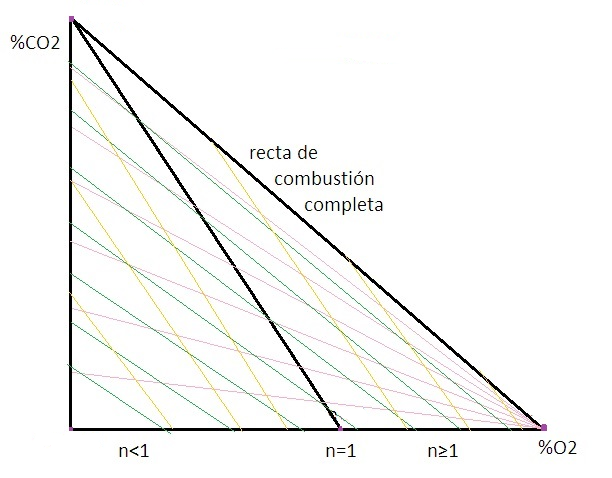
\includegraphics[width=\linewidth]{res/tema2/oswaldo}
						\label{fig:oswaldo}
					\end{minipage}%
					\begin{minipage}{0.4\linewidth}
						\centering
						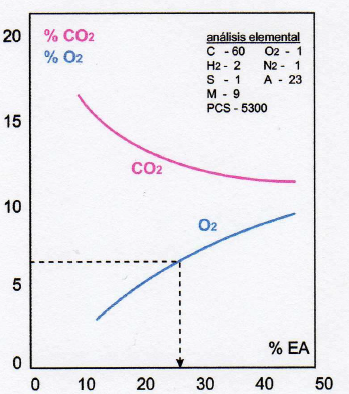
\includegraphics[width=\linewidth]{res/tema2/CO2O2}
						\label{fig:co2o2}
					\end{minipage}
				\end{figure}
				\item [-] \textbf{Balance energético en la caldera:} Se deben tener en cuenta las características energéticas y gasto del combustible frente a la calidad del vapor generado.
				
				
				Las principales pérdidas de calor en la caldera se deben a:
				\begin{itemize}
					\item Combustión incompleta: Se reduce a medida que se aumenta el exceso de aire.
					\item Calor sensible de los gases de escape: Aumenta a medida que se aumenta el exceso de aire.
					\item Sólidos inquemados: Disminuye a medida que se aumenta el exceso de aire.
				\end{itemize}
				Que resumido en un gráfico queda:
				\begin{figure}[H]
					\centering
					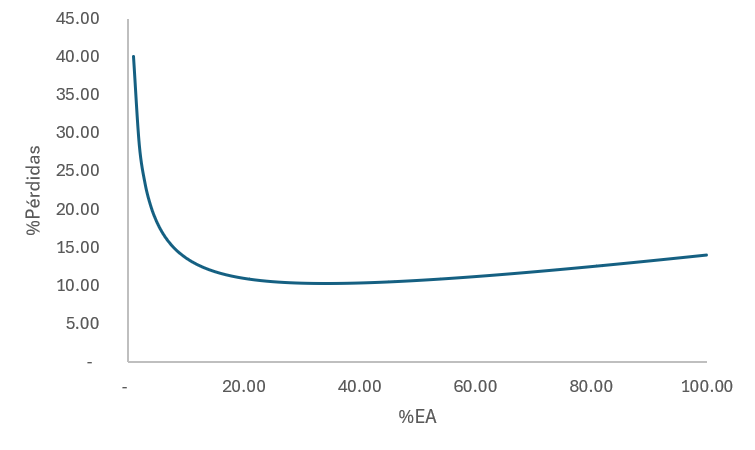
\includegraphics[width=0.5\linewidth]{res/tema2/perdidas}
					\label{fig:perdidas}
				\end{figure}
				Por tanto, el rendimiento de la caldera queda como:
				\[\eta = \frac{\text{Potencia térmica cedida al vapor sobrecalentado de salida}}{PCI \times \dot{m}_\text{combustible} \times \text{Potencia térmica aire caliente}}\approx 85-88\%\]
				En general en la caldera hay varios rendimientos:
				\begin{figure}[H]
					\centering
					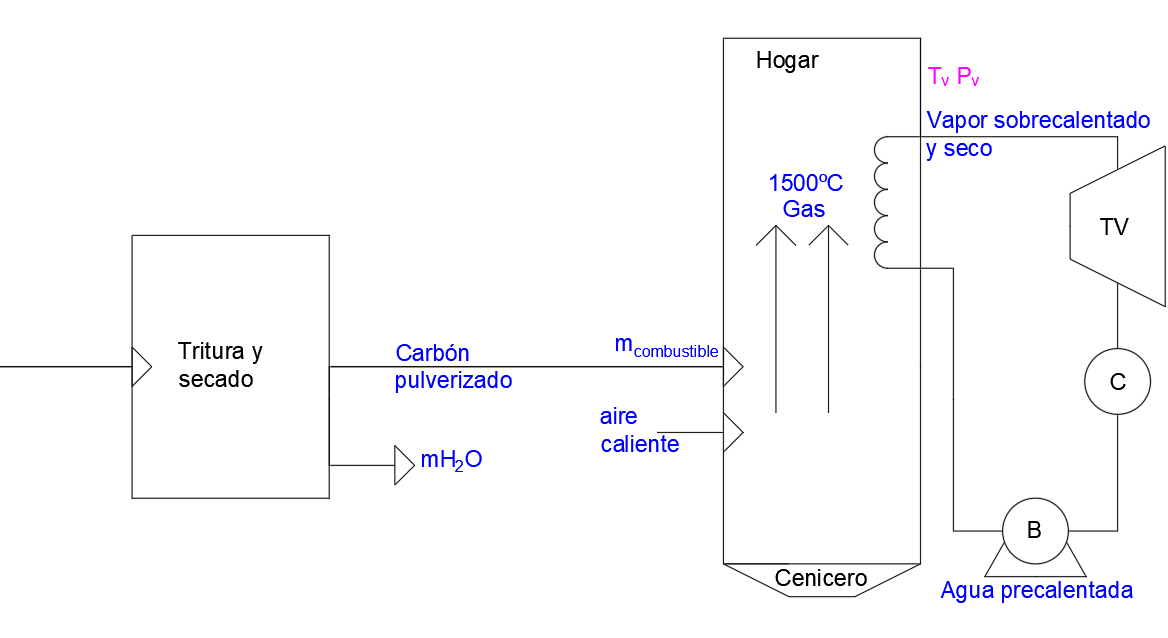
\includegraphics[width=0.7\linewidth]{res/tema2/caldera}
					\label{fig:caldera}
				\end{figure}
				Los distintos rendimientos son:
				\[\eta_{caldera}=\frac{P_{tv}}{P_{tv}+P_{aire}}\]
				\[P_{tv}=\dot{m}_{comb}\times PCI\]
				\[P_{aire}=\dot{m}_{aire}\times h_{aire}\]
				\[\eta_{planta}=\frac{P_{bc}}{P_{comb}}\]
		\end{itemize}
\end{enumerate}
\subsection{Combustible gaseosos.}
Principalmente gases naturales y materia volátil. Son de fácil combustión (poco exceso de aire). Emiten NO$_x$ y SO$_2$. Tienen peligro de explosión y por ello, requieren elevada estanqueidad.
\subsection{Combustible líquidos.}
Se compone de mezclas complejas de hidrocarburos de cadena larga. Tienen un punto de inflamación baja. Emiten NO$_x$ y SO$_2$. Provocan corrosión a baja temperatura.

\section{Impacto ambiental de las centrales térmicas de combustión.}
\subsection{Composición de gases de la combustión.}
\begin{enumerate}
	\item \textbf{Monóxido de carbono (CO):}
		Se produce por combustiones incompletas de compuestos que contienen carbono. Es un gas muy tóxico. En contacto con el oxígeno forma CO$_2$.
	\item \textbf{Materia particulada (PM):}
		Son mineral, inquemados y elementos de traza.
		\begin{itemize}
			\item [-] Una cuarta parte se recoge como ceniza mediante los ceniceros. El resto es liberado y se captura con filtros ciclónicos o electrostáticos.
			\item [-] Los elementos de traza (Hg y Se) se capturan mediante filtros de resinas.
		\end{itemize}
		Los minerales que se consideran contaminantes son:  Be, Cr, Mn, Co, Ni, As, Se, Cd, Sb, Hg y Pb.
	\item \textbf{Compuestos orgánicos:}
		Se pueden encontrar como gas si son volátiles (metano y benceno) o en la superficie de partículas como hidrocarburos aromáticos policlínicos.
	\item \textbf{Óxidos de azufre (SO$_2$, SO$_3$, SH$_2$):}
		Provocan lluvia ácida. En las calderas se forma SO$_2$ que posteriormente forma el resto de óxidos.
		\begin{figure}[H]
			\centering
			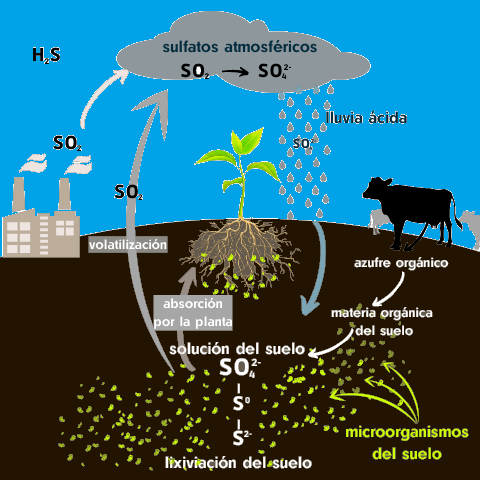
\includegraphics[width=0.4\linewidth]{res/tema2/sicloazufgre}
			\label{fig:sicloazufgre}
		\end{figure}
		
	\item \textbf{Óxidos de nitrógeno (NO$_x$):}
		Provocan lluvia ácida, destrucción de la capa de ozono y smog fotoquímico:
		\begin{itemize}
			\item [-] \textbf{NO$_2$:} precursor del efecto invernadero. Son muy absorbentes de radiación infrarroja. Se genera a partir del NO con exceso de oxígeno.
			\item [-] \textbf{NO:} reducción del ozono en la estratosfera (es menos tóxico que el NO$_2$). Se genera por la alta temperatura de la caldera con el N$_2$ del aire. 
			\item [-] \textbf{N$_2$O:} reducción del ozono en la troposfera. Se produce en mezclas pobres con poco O$_2$.
		\end{itemize}
\end{enumerate}
\subsection{Tratamientos para reducción de emisiones.}
\begin{enumerate}
	\item \textbf{Óxidos de azufre (SO$_2$):}
	Se clasifican en función del momento de la combustión en el que se realice el tratamiento:
	\begin{enumerate}
		\item \textbf{Precombustión:} 
		\begin{itemize}
			\item [-] Uso de carbones de alta calidad.
			\item [-] Combustión mixta con gas natural.
			\item [-] Lavado y desulfuración del combustible.
			\item [-] Gasificación del carbón.
		\end{itemize}
		\item \textbf{Durante la combustión:}
		\textbf{Solo en calderas de lecho fluidificado} se puede introducir caliza CaCO$_3$ para fijar el azufre. 
		\item \textbf{Postcombustión:}
			Se manipulan los gases mediante torres de lavado por vía húmeda o semihumeda con un rendimiento del 40\%.
			
			El proceso de absorción química en las torres de lavado es el siguiente:
			\[SO_2+H_2O\rightarrow H_2SO_4\]
			\[CaCO_3+H_2SO_4\rightarrow CaSO_3+CO_2+H_2O\]
			\[CaSO_3+0,5O_2+H_2O\rightarrow CaSO_4+2H_2O\]
			\begin{figure}[H]
				\centering
				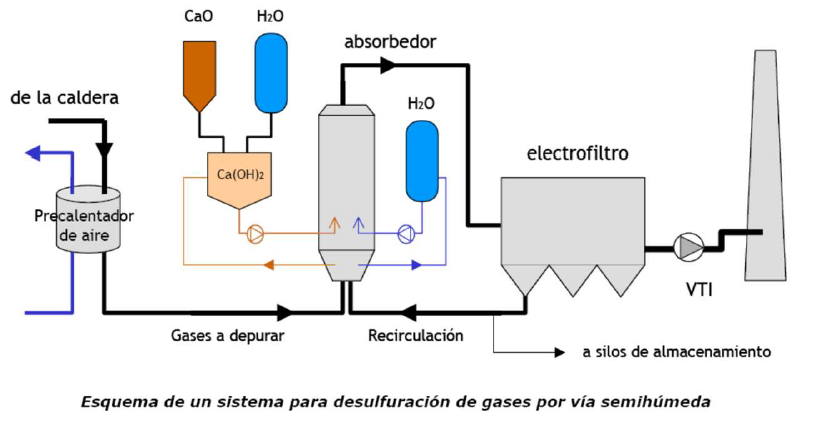
\includegraphics[width=0.5\linewidth]{res/tema2/desulfuric}
				\label{fig:desulfuric}
			\end{figure}
			
	\end{enumerate}
	\item \textbf{Óxidos de nitrógeno (NO$_x$):}
	\begin{itemize}
		\item [-] \textbf{Técnicas primarias:} Se basan en el control del proceso de combustión. Modificacando los siguientes parámetros que reducen las emisiones de NO$_x$ a costa del rendimiento:
		\begin{itemize}
			\item Reducción de la temperatura.
			\item Disminución del exceso de aire.
			\item Inyección de vapor.
			\item Combustión con O$_2$ puro.
			\item Combustible con menos N$_2$.
			\item Uso de catalizadores.
		\end{itemize}
		El problema de los NO$_x$ disminuye en las calderas de lecho fluido debido a que trabajan a 900° C en lugar de los 1500° C de una caldera convencional.
		\item [-] \textbf{Técnicas secundarias:} Se basan en reducir las emisiones de gases tras la combustión:
		\begin{itemize}
			\item Absorción química con $H_2SO_4$:
			
\begin{figure}[H]
	\centering
	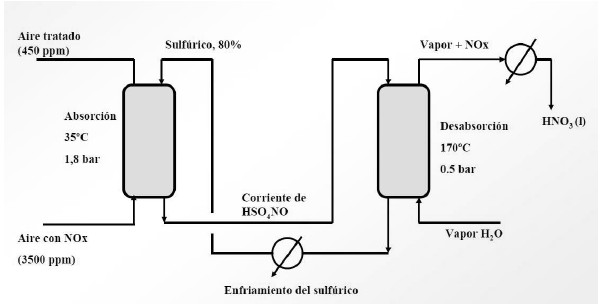
\includegraphics[width=0.5\linewidth]{res/tema2/H2so4abs}
	\label{fig:h2so4abs}
\end{figure}
	\item Proceso TYCO: incorpora eliminación $SO_2$ y recupera ácidos:
	
\begin{figure}[H]
	\centering
	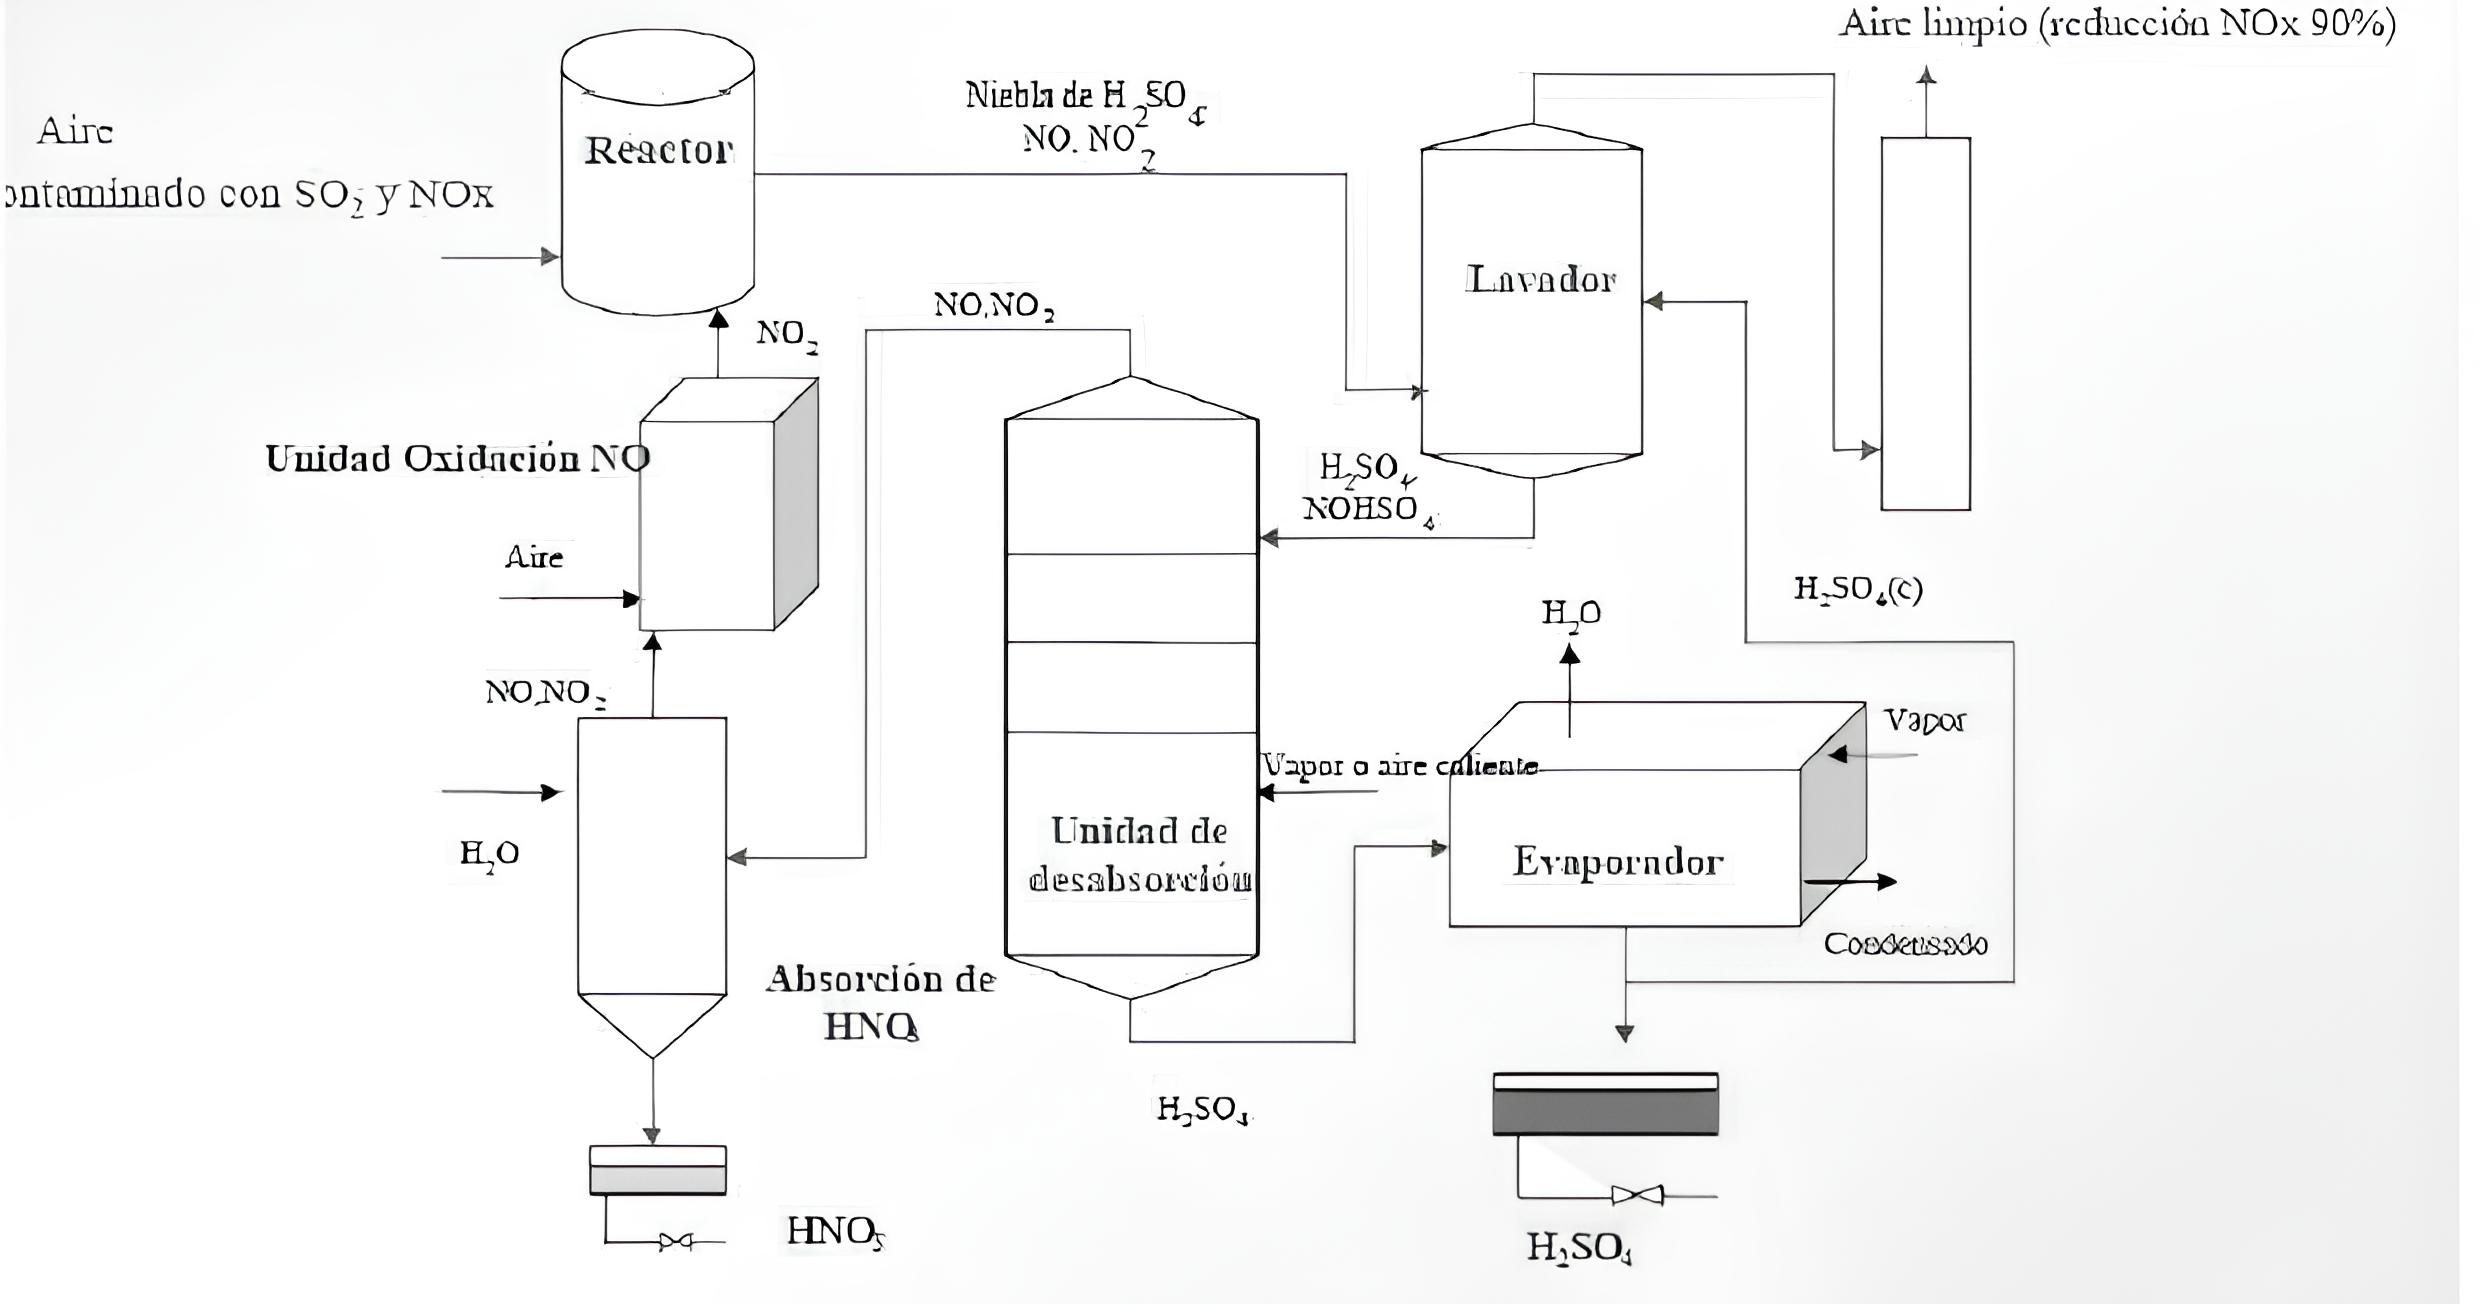
\includegraphics[width=0.5\linewidth]{res/tema2/tyci+}
	\label{fig:tyci}
\end{figure}
\item Reducción catalítica selectiva: se emplea amoniaco que al reaccionar con los NO$_x$. Tiene una eficiencia de eliminación del 85\%.
\[6NO_x+4xNH_3\rightarrow [2x+3]N_2+6xH_2O\]
		\end{itemize}
	\end{itemize}
	\item \textbf{Materia particulada (PM):} Se trata mediante filtros ciclónicos y electrostáticos tras la combustión. Tienen un gran consumo energético 12\% del autoconsumo.
\end{enumerate}
\begin{figure}[H]
	\centering
	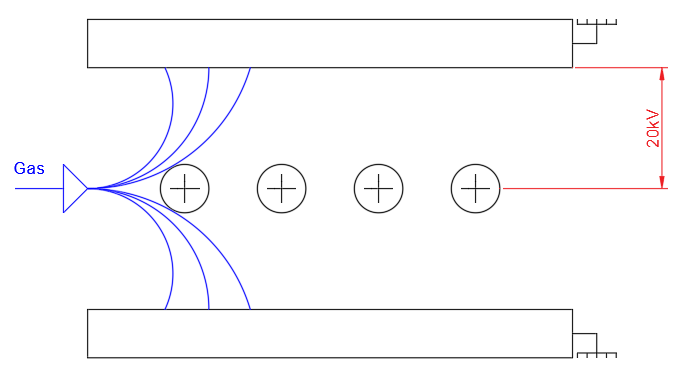
\includegraphics[width=0.7\linewidth]{res/tema2/filtroelectrostatico}
	\label{fig:filtroelectrostatico}
\end{figure}

\subsection{Impacto ambiental centrales térmicas.}
Anteriormente se han discutido principalmente las centrales térmicas de carbón, pero si el combustible es líquido o sólido cambia ligeramente el impacto ambiental.
\begin{itemize}
	\item \textbf{Combustible líquido:}
		El impacto ambiental es menor que el de las de carbón aunque el uso de estas centrales esta disminuyendo. Emite menos gases contaminantes y la materia particulada esta compuesta principalmente por hollín. 
		
		
		Los combustibles principales usados son los gasóleos (comparten mercado con la automoción) y los fuelóleos (uso exclusivo en instalaciones térmicas).
		
		El principal inconveniente de los fuelóleos es su alto contenido en azufre.
	\item \textbf{Gas natural:}
		El gas natural es un combustible con muy alto poder calorífico y son las centrales de combustión de combustibles fósiles con menor impacto ambiental aunque tienen problemas de emisiones de NO$_x$ y generan elevada contaminación acústica.
		
		Cabe destacar, que otra ventaja es que como se recibe continuamente gas no es necesario invertir en sistemas de almacenamiento y, además, no necesita tratamiento previo. Que también como durante el transporte se entierran la contaminación producida por fugas es despreciable.
\end{itemize}
\section{Impacto ambiental centrales nucleares.}
Tienen el mismo impacto térmico y químico que las centrales térmicas convencionales aunque no libera gases contaminantes. No obstante, presenta el problema de los residuos radioactivos.
\subsection{Tipos de radioactividad.}
La radioactividad es un efecto producido por descomposición espontánea de un núcleo inestable en otro más estable. Los tipos de radiación principales son:
\begin{itemize}
	\item [-] La radiación alfa ($\alpha$) está formada por núcleos de helio. No es capaz de atravesar el papel.
	\item [-] La radiación beta ($\beta$) está constituida por electrones. No es capaz de atravesar el acero.
	\item [-] La radiación gamma ($\gamma$) es de naturaleza electromagnética. No es capaz de atravesar el plomo.
	\item [-] Radiación neutrónica (n). No es capaz de atravesar el cemento.
\end{itemize}
\subsection{Medida de la radioactividad.}
Se mide mediante la cantidad de radiación emitida. 
\begin{itemize}
	\item [-] Si la radiación afecta al ser humano se mide en Sievert (Sv): Unidad de dosis equivalente.
	\item [-] Si la radiación afecta a un objeto se mide en Gray (Gy): Unidad de dosis absorbida. Se define como la dosis de radiación que transfiere una energía de 1 julio a 1 kilogramo masa de
	material irradiado
	\item [-] Si se habla de fuente emisora de radiación (material radiactivo) se emplea el Becquerel (Bq). Se define como la actividad de un material que experimenta una desintegración por segundo.
	
\begin{figure}[H]
	\begin{center}
	\scalebox{0.8}[0.8]{
		\begin{tikzpicture}
			\def\printonlylargeenough#1#2{\unless\ifdim#2pt<#1pt\relax
				#2\printnumbertrue
				\else
				\printnumberfalse
				\fi}
			\newif\ifprintnumber
			\pie[rotate=90, text=legend, before number=\printonlylargeenough{1}, after number=\ifprintnumber\%\fi]{
				36.7/Inhalación de radón,
				29.1/Aplicaciones médicas,
				13.1/Radiación suelo,
				10.2/Radiación cosmica,
				9.9/Propio Cuerpo,
				0.6/Exposición profesional: 0.6\%,
				0.3/Poso radioactivo 0.3\%,
				0.1/Centrales nucleares 0.1\%
			}
		\end{tikzpicture}
}	\end{center}
\end{figure}	
\end{itemize}
\subsection{Clasificación de los residuos radioactivos.}
\begin{itemize}
	\item [-] \textbf{Según el estado de agregación.}
	\begin{enumerate}
		\item \textbf{Residuos gaseosos:} Se debe distinguir entre isotopos radioactivos y el aire. Mediante filtros de alta eficiencia (HEPA) se retiene el 99,9\% de las partículas de 0,3 $\mu$m.
		\item \textbf{Residuos líquidos:} Principalmente tritio. Se eliminan con operaciones de filtración, centrifugación, precipitación química,
		intercambio iónico y evaporación .
		\item \textbf{Residuos sólidos:} Se clasifican en alta, media o baja actividad.
	\end{enumerate}
	\item [-] \textbf{Según la radiactividad.}
	\begin{enumerate}
		\item \textbf{Sólidos de actividad media y baja:} Tienen una vida media de menos de 30 años. Se mezclan con aglomerantes y se almacenan en depósitos. 
		
		España genera 1220 m$^3$ al año. Los residuos dejan de ser peligrosos a los cientos de años con lo cual es seguro almacenarlos en instalaciones permanentes en superficie. 
		\item \textbf{Sólidos de alta actividad:} Están constituidos por el combustible gastado. Contienen radionucleidos de larga vida media que tardan miles de años en llegar a niveles seguros de radiación. 
		
		Se enfrían en piscinas en la propia central durante 5 años y después se embuten en vidrio para ser almacenados en lugares de almacenamiento centralizado. Actualmente en España estos residuos se almacenan en el extranjero con un coste de 49.545,17€/día (en teoria deberian haber vuelto a España en 2010).
	\end{enumerate}
	La generación media de una central tipo de 1.000 MW es de 20 toneladas de uranio al
	año (combustible gastado), de 50 m$_3$ (centrales con tecnología PWR) y 130 m$^3$
	(centrales BWR) de residuos de media y baja actividad.
	
	Anteriormente el precio de la gestión de los residuos radiactivos recaía sobre el consumidor de la energía eléctrica. No obstante, actualmente se plantea que las nucleares paguen esta gestión.
\end{itemize}
\subsection{Gestión del combustible gastado.}
Cuando se descarga el combustible del reactor todavía hay gran cantidad de energía puede ser utilizada al solo haberse gastado el 5\% de la energía inicial.
\begin{itemize}
	\item [-] Si se almacena tras su uso en instalaciones de almacenamiento geológico profundo se habla de ciclo abierto.
	\item [-] Si se reprocesa el combustible gastado para ser reutilizado se habla de ciclo cerrado. En el ciclo cerrado se recupera el combustible fabricando pastillas de óxido de uranio (UO$_2$) y óxido de plutonio (PuO$_2$) que se denominan combustible MOX.
\end{itemize}
Las piscinas donde se almacena el combustible gastado suelen ser de agua por su alto coeficiente de transmisión del calor y sus propiedades como blindaje. Hoy en día presentan una problemática debido a que las piscinas de las centrales nucleares españolas están saturadas.
\section{Impacto ambiental centrales hidroeléctricas.}
De acuerdo con la IHA (International Hydropower Association), existen varios aspectos clave que hay que tener en
cuenta para mantener el potencial hidroeléctrico con un desarrollo sostenible en materia medioambiental:
\begin{enumerate}
	\item \textbf{Calidad del agua:} Puede reducir la cantidad de oxígeno en agua, su temperatura y la estratificación de los sedimentos.
	\item \textbf{Erosión y transporte de sedimentos:} Cambia la cantidad de sedimentos transportados y a largo plazo puede cambiar la forma del río por el cambio de la erosión.
	\item \textbf{Hidrología y flujos mediambientales del río:} Como cambia la hidrología y el entorno del río afecta a la fauna y a actividades humanas que se desarrollaban en el río.
	\item \textbf{Especies en peligro de extinción:}  La construcción de una presa puede poner en serio riesgo a especies amenazadas o únicas, debido a los
	cambios del hábitat natural.
	\item \textbf{Paso de especies:} Muchas especies recorren el río a lo largo de su ciclo de vida en uno o ambos sentidos. En muchos lugares,
	la migración de peces (como el salmón) es un acontecimiento anual, que se ve seriamente dificultado por las
	presas.
	\item \textbf{Plagas animales y vegetales en los embalses:} Los cambios en las condiciones del agua pueden facilitar la colonización de especies
	ajenas al entorno, creando plagas.
	\item \textbf{Aspectos sanitarios:} Los cambios producidos en el entorno por la construcción de presas pueden afectar a la salud pública,
	influyendo en la transmisión de enfermedades.
	\item \textbf{Actividades de construcción:} Las actividades de construcción provocan alteraciones en el medio acuático y terrestre.
\end{enumerate}
\section{Impacto ambiental transporte y transformación energía eléctrica.}
Tienen un impacto menor que las instalaciones de producción.
\begin{enumerate}
	\item \textbf{Líneas de transporte y distribución:} Se utilizan terrenos para la instalación de torres que provocan impacto visual y afectan a la avifauna.
	\item \textbf{Subestaciones de transformación:}
	Provocan una pérdida de suelo y vegetación, emiten ruidos y pueden provocar contaminación de agua por fugas.
	\item \textbf{Redes de baja tensión y centros de transformación:} Producen impacto visual y emisión de ruidos.
	\item \textbf{Campos electromagnéticos:} Los campos eléctricos son proporcionales a la tensión y los campos magnéticos a la intensidad.	
\end{enumerate}
		\section{Tema 3: Conservación de la masa}
\subsection{Teorema del transporte de Reynolds}
\begin{figure}[H]
	\centering
	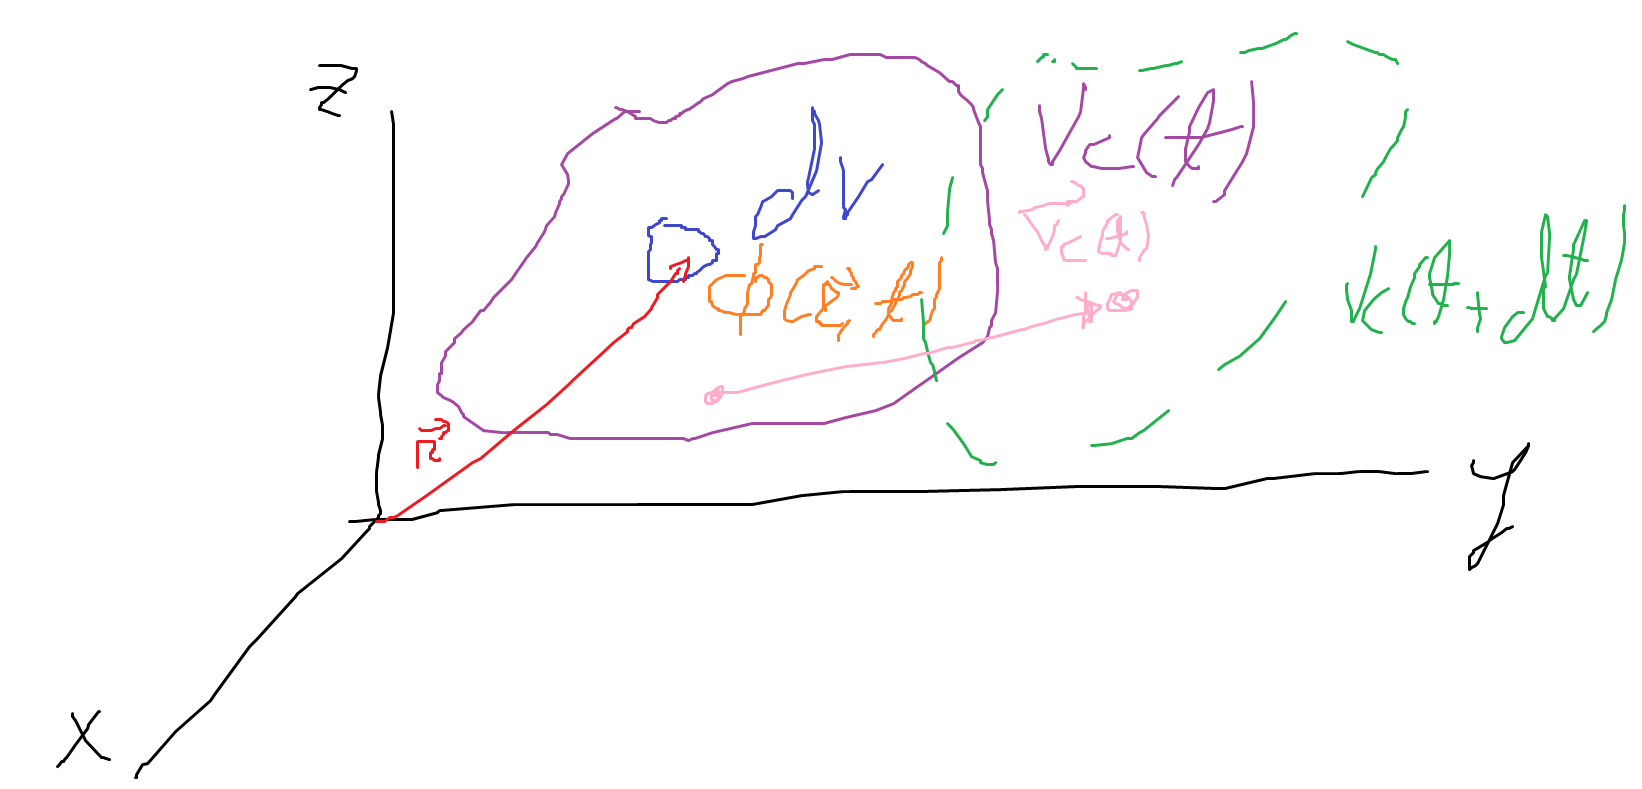
\includegraphics[width=0.7\linewidth]{imagenesTema3/magnitudesReynolds}
	\caption{}
	\label{fig:magnitudesreynolds}
\end{figure}

\[\Phi=\text{Función que depende del espacio y tiempo en general}\rightarrow\Phi=f(\vec{r},t)\]

Nos interesa conocer:
\[\frac{d}{dt}\int_{V_c(t)} \Phi(\vec{r},t) \,dV=\lim_{\Delta t \to 0} \left[\int_{V_c(t+dt)} \Phi(\vec{r},t+dt) \,dV-\int_{V_c(t)} \Phi(\vec{r},t) \,dV\right]\]
Se hace el desarrollo de Taylor en t del primer término:
\[\frac{d}{dt}\int_{V_c(t)} \Phi(\vec{r},t) \,dV=\int_{V_c(t)} \frac{\partial}{\partial t}\Phi(\vec{r},t) \,dV+\lim_{\Delta t \to 0} \frac{1}{\Delta t}\left[\int_{V_c(t+dt)} \Phi(\vec{r},t) \,dV-\int_{V_c(t)} \Phi(\vec{r},t) \,dV\right]\]

Hay que estudiar la velocidad del volumen de control de tal manera que, solo afecta la velocidad paralela a la normal porque es lo que provoca expansión o compresión del mismo, la velocidad tangencial lo "gira":
\[dV=\vec{v}_c\cdot\vec{n}dS\Delta t\]
Por tanto:
\[\frac{d}{dt}\int_{V_c(t)} \Phi(\vec{r},t) \,dV=\int_{V_c(t)} \frac{\partial}{\partial t}\Phi(\vec{r},t) \,dV+\oint_{S_c(t)} \Phi(\vec{r},t)\vec{v}_c\cdot\vec{n}\Delta t \,dS\]

Si queremos podemos imponer que (hablando en tema de volumen fluido):
\[V_c(t)=V_{fluido}(t)=V_f(t)\]
\[\frac{d}{dt}\int_{V_f(t)} \Phi(\vec{r},t) \,dV=\int_{V_f(t)} \frac{\partial}{\partial t}\Phi(\vec{r},t) \,dV+\oint_{S_f(t)} \Phi(\vec{r},t)\vec{v}\cdot\vec{n}\Delta t \,dS\]

Si tomamos un tiempo t* paramétrico tal que $V_c(t*)=V_F(t*) \rightarrow \int_{V_c(t*)}\frac{\partial \Phi}{\partial t}\,dV\approx \int_{V_f(t*)}\frac{\partial \Phi}{\partial t}\,dV$ Solo en ese instante t*

Si se restan las ecuaciones de Volumen de control y la de los movimientos fluidos queda (Teorema de Reynolds del transporte (problemas)):

\[\frac{d}{dt}\int_{V_f(t)}\Phi(\vec{r},t)\,dV=\frac{d}{dt}\int_{V_c(t)}\Phi(\vec{r},t)\,dV+\oint_{S_c(t)} \Phi(\vec{r},t)\left[(\vec{v}-\vec{v}_c)\cdot\vec{n}\right]\Delta t \,dS\]

(TH Reynolds para teoria)
\[\frac{d}{dt}\int_{V_f(t)} \Phi(\vec{r},t) \,dV=\int_{V_f(t)} \frac{\partial}{\partial t}\Phi(\vec{r},t) \,dV+\oint_{S_f(t)} \Phi(\vec{r},t)\vec{v}\cdot\vec{n}\Delta t \,dS\]

Término de variación local:
\[\int_{V_f(t)} \frac{\partial}{\partial t}\Phi(\vec{r},t) \,dV\]
Térimno de variación convectiva:
\[\oint_{S_f(t)} \Phi(\vec{r},t)\vec{v}\cdot\vec{n}\Delta t \,dS\]


Si la magnitud $\Phi = \rho$ Se obtiene la ecuación de conservación de la masa en forma integral:
Es igual a 0 porque no se pierde masa:
(Problemas)
\[\frac{d}{dt}\int_{V_f(t)}\rho\,dV=\frac{d}{dt}\int_{V_c(t)}\rho\,dV+\oint_{S_c(t)} \rho\left[(\vec{v}-\vec{v}_c)\cdot\vec{n}\right]\Delta t \,dS=0\]
(Teoría)
\[\frac{d}{dt}\int_{V_f(t)} \rho \,dV=\int_{V_f(t)} \frac{\partial \rho}{\partial t} \,dV+\oint_{S_f(t)} \rho\vec{v}\cdot\vec{n}\Delta t \,dS=0\]

Si $V_f(t)\approx dV_f(t)$ entonces y aplicando el teorema de gauss se llega a la ecuación diferencial de la masa o forma conservativa:
($\oint_S \varphi \cdot \vec{n}\,dS=\int_V \vec{\nabla}\cdot\varphi\,dV$)
\[\lim_{dV \to 0}\left[\frac{\partial \rho}{\partial t} dV+\vec{\nabla}\cdot\left(\rho\vec{v}\right)dV\right]=0\]
\[\frac{\partial \rho}{\partial t} +\vec{\nabla}\cdot\left(\rho\vec{v}\right)=0\]
Término local de masa: 
\[\frac{\partial \rho}{\partial t}\]
Término convectivo de masa:
\[\vec{\nabla}\cdot\left(\rho\vec{v}\right)\]

		\chapter{Cobertura de la demanda. Mercado eléctrico.}
\section{Explotación del mercado eléctrico.}
La energía eléctrica se genera en grandes concentradas de forma concentrada y posteriormente se transmite a grandes distancias donde el equilibrio se obtiene de las curvas de oferta y demanda.


Una misión importante de la red es la de ajustar la energía generada a la demandada con unos valores de tensión (Control Q-U) y frecuencia (Control P-f).
\section{Curva de demanda diaria.}
La demanda varia constantemente tanto hora a hora como diariamente. Esta demanda se refleja en las curvas de carga o demanda donde la diferencia entre ambas equivale a las pérdidas en la red ($\approx$12\%).

\begin{itemize}
	\item [-]\textbf{Energía producida:} se entiende en barras de la central, descontando el autoconsumo.
	\item [-]\textbf{Energías consumida:} se obtiene de la suma del consumo de los abonados.
\end{itemize}
\begin{figure}[H]
	\begin{minipage}{0.5\linewidth}
		\centering
		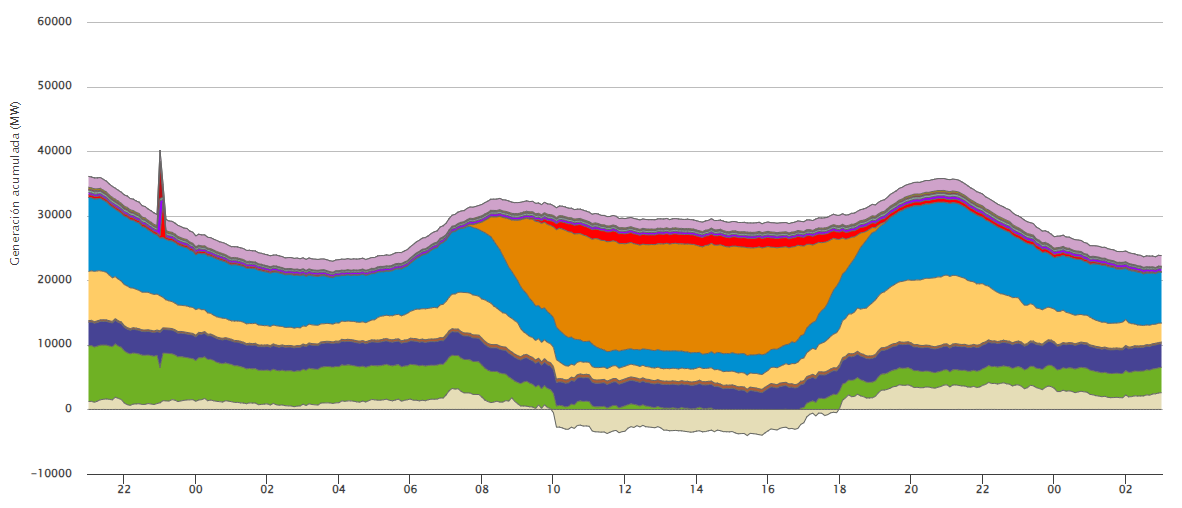
\includegraphics[width=0.7\linewidth]{res/tema4/demandaDia}
		\label{fig:demandadia}
	\end{minipage}
	\begin{minipage}{0.5\linewidth}
		\centering
		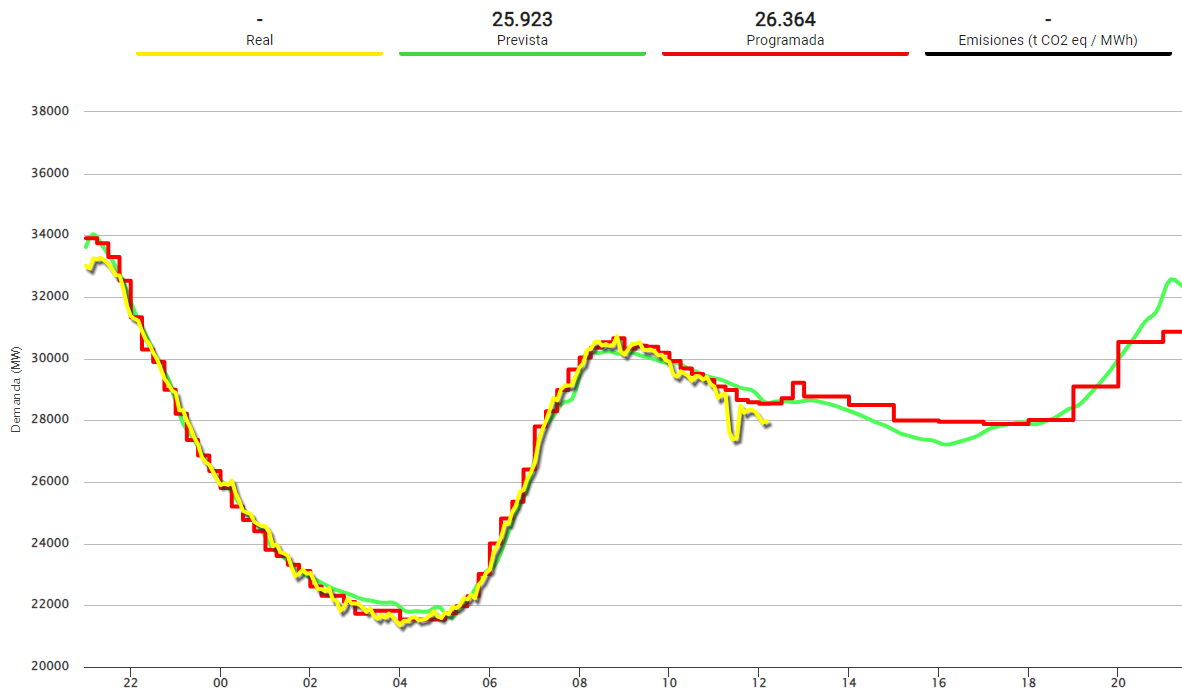
\includegraphics[width=0.7\linewidth]{res/tema4/demandaDia1}
		\label{fig:demandadia1}
	\end{minipage}
\end{figure}
La curva de carga o de demanda se predice mediante la estadística acumulada de muchos años ya que para fijar el precio es necesaria esta previsión (tiene un error asociado del 2\%). En estos datos, se pueden apreciar típicamente tres picos de consumo (12, 16 y 20 horas) que llevan a la tarifa PVPC (Precio de venta al pequeño consumidor) con discriminación horaria en horas valle, llano y punta.


Cabe destacar, como los factores locales tienen mucho peso sobre la demanda real como la temperatura, grandes eventos, ...

\section{Pérdidas en la red.}
Son un coste de operación necesario para mover la energía desde donde se produce (Galicia y Cataluña como pozos) hacia donde se consume (Madrid y Barcelona como sumideros). 
\begin{itemize}
	\item [-] Red de transporte 1-2\%
	\item [-] Red de distribución 4-6\%
	\item [-] Red baja tensión 7-10\%
\end{itemize}
\section{Gestión de la red.}
La empresa encargada de la gestión de la red es Red Eléctrica Española (REE) que recibe a través de su red de fibra óptica las potencias activa y reactiva en varios puntos de la red. La gestión se realiza desde el Centro de Control Eléctrico (CECOEL).

Para realizar esta gestión REE debe tener en cuenta muchas incertidumbres asociadas a defectos en generadores y la red lo cual provoca un sobredimensionamiento del sistema.
\subsection{Incidencias no previstas.}
Cuando ocurren incidencias graves, normalmente asociadas a una falta en la generación REE debe aplicar cortes a las industrias acogidas a contratos de interrumpibilidad.
\subsection{Configuración sistema eléctrico de potencia.}
El sistema léctrico de potencia se compone de lo siguientes elementos:
\begin{itemize}
	\item [-] \textbf{Generación:} Se genera en barras del generador de 6-30 kV a 50Hz con potencias de hasta 1500 MVA.
	\item [-] \textbf{Redes de Transporte:} Esta formada por un elevado número de nodos con topología mallada a los que se conectan los generadores y consumidores a una tensión de 220-400kV.
	\item [-] \textbf{Redes de Distribución:}  Las longitudes de estas líneas no superan los 25 km y normalmente son aéreas. En núcleos urbanos suelen ser malladas y en zona rural radiales. Se distribuye de 132-15kV.
	\item [-] \textbf{Centros de transformación:} Se reduce la tensión de media a baja tensión.
	\item [-] \textbf{Consumidores:} Red de distribución a 230/400V.
\end{itemize}
\section{Funcionamiento del mercado eléctrico.}
Desde la Ley 54/1997 se liberalizó el sector eléctrico para permitir la libre competencia con las siguientes características:
\begin{itemize}
	\item [-] Libertad de construcción de nuevas centrales de producción de electricidad.
	\item [-] Competencia entre las empresas productoras de electricidad en un mercado de ofertas.
	\item [-] Libertad progresiva de los consumidores para elegir el suministrador que deseen y acordar con
	él las condiciones y precio del kWh.
	\item [-] Libertad de comercialización de la electricidad.
	\item [-] Libertad de comprar o vender electricidad a empresas y consumidores de otros miembros de
	la UE.
	\item [-] Separación jurídica de actividades:
	\begin{itemize}
		\item \textbf{Reguladas:} transporte, distribución y gestión del sistema.
		\item \textbf{No reguladas:} generación y comercialización
	\end{itemize}
	\item [-] Sostenibilidad económica y financiera:
	\begin{itemize}
		\item Garantizar el suministro al mínimo coste.
		\item Retribución de actividades con base en criterios objetivos, transparente y homogéneos.
		\item Marco normativo que garantice la estabilidad financiera.
		\item  Actualización de los peajes de acceso a través de cargos.
	\end{itemize}
\end{itemize}
La explotación del mercado eléctrico se realiza conjuntamente entre:
\begin{itemize}
	\item 
	\item
	\item
\end{itemize}
\subsection{Actividades principales.}
g
\subsection{Reparto de la distribución de energía eléctrica.}
g
\subsection{Comercialización.}
g
\subsection{Organización.}
g
\subsection{Instituciones reguladoras.}
g
\subsection{Operador del mercado (OMIE).}
g
\subsection{Operador del sistema (REE).}
g
\section{Mercado ibérico (MIBEL).}
g
\section{Interconexiones con el extranjero.}
g
\subsection{Francia.}
g
\subsection{Portugal.}
g
\subsection{Marruecos.}
g
\subsection{Gestión de las interconexiones.}
g
\section{Mercado intradiario.}
g
\subsection{Secuencia de los procesos del mercado.}
g
\subsection{Mercados a plazo.}
g
\subsection{Mercado organizado diario (casación horaria).}
g
\subsection{Tipos de oferta de venta de energía.}
g
\subsection{Proceso de casación.}
g
\subsection{Curva de oferta de venta de energía.}
g
\subsection{Influencia fuentes renovables.}
g
\subsection{Retribuciones para amortizar costes fijos.}
g
\subsection{Curva de demanda.}
g
\section{Mercado de restricciones técnicas.}
g
\section{Mercado de servicios complementarios.}
g
\subsection{Regulación primaria.}
g
\subsection{Regulación secundaria.}
g
\subsection{Control de tensión.}
g
\subsection{Reservas de potencia.}
g
\subsection{Gestión de desvíos.}
g
\subsection{Regulación terciaria.}
g
\section{Precio medio final.}
g
\subsection{Costes recogidos en la tarifa eléctrica (PVPC).}
g
\section{Programación de la generación de electricidad.}
g
\subsection{Curva acumulada de demanda anual.}
g
\subsection{Curva de demanda anual.}
g
\subsection{Parámetros principales curva de demanda.}
g
\subsection{Curva acumulada de generación anual.}
g
\subsection{Parámetros principales curva de generación.}
g
\section{Reserva de potencia.}
g
\subsection{Características estáticas.}
g
\subsection{Características dinámicas.}
g
\subsection{Secuenciamiento óptimo de grupos.}
g
\section{Costes de generación.}
g
\subsection{Comparativa de costes.}
g
\subsection{Coste de inversión o fijo.}
g
\subsection{Costes variables.}
g
\subsection{Coste total.}
g
\section{Aspectos técnicos de la producción de energía.}
g
		\chapter{Selectividad interruptores automáticos de baja tensión}
En caso de defecto debe abrir el interruptor automático situado inmediatamente aguas arriba del defecto y sólo él.
\begin{figure}[H]
	\centering
	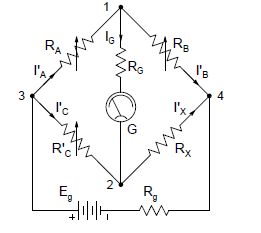
\includegraphics[width=0.4\linewidth]{Images/18}
\end{figure}
\section{Selectividad Total}
Para cualquier valor de la intensidad de defecto “aguas abajo” de B, el interruptor automático B es el único en desconectar 
\section{Selectividad Parcial}
Para ciertos valores de la intensidad de defecto “aguas abajo” de B, el interruptor B es el único en desconectar, pero para otros abren los dos interruptores, A y B
\section{Selectividad frente a sobrecargas}
\section{Selectividad frente a cortocircuitos}
\section{Selectividad frente a cortocircuitos moderados}
\section{Coordinación entre interruptores automáticos}
\section{Selectividad lógica}
		\chapter{Generador síncrono.}

	\section{Generalidades.}
		Los generadores síncronos o alternadores trifásicos autoexcitados en corriente continua que se usan en las centrales eléctricas se diferencian en función del número de vueltas de sus máquinas motrices.
		
		
		Velocidad síncrona en régimen permanente:
		
		\[n = \dfrac{60\cdot f}{p}\,[rpm]\]
		
		Donde $f$ es la frecuencia industrial y $p$ el número de pares de polos.
		
		
		\subsection{Aplicaciones de la máquina síncrona.}
			\begin{itemize}
				\item \textbf{Como generador:}
					\begin{itemize}
						\item Suministro de potencia a la red.
						\item Suministro de emergencia (hospitales, centros comerciales...).
						\item Instalaciones aisladas (redes rurales).
					\end{itemize}
					
				\item \textbf{Como motor:}
					\begin{itemize}
						\item Aplicaciones con velocidad constante (bombeo en centrales hidráulicas reversibles).
						\item Compensador síncrono en centrales (regulación del factor de potencia).
					\end{itemize}
			\end{itemize}
			
		\subsection{Aspectos constructivos.}
			\begin{itemize}
				\item \textbf{Inducido:}
					\begin{itemize}
						\item Se alimenta con corriente alterna trifásica.
						\item Con expansiones polares y devanado concentrado.
						\item Cilíndrico y con devanado concentrado o distribuido.
						\item Generalmente conectado en Y, con el neutro puesto a tierra.
					\end{itemize}
				
				\item \textbf{Inductor:}
					\begin{itemize}
						\item Se alimenta en corriente continua mediante anillos rozantes.
						\item \textit{Polos salientes:} devanado concentrado con devanado amortiguador (barras de cobre cortocircuitadas) para reducir oscilaciones pendulares y facilitar el arranque.
						\item \textit{Polos lisos o rotor cilíndrico:} devanado distribuido en ranuras.
					\end{itemize}
			\end{itemize}
				
			\begin{table}[H]
				\centering
				\renewcommand{\arraystretch}{1.1}
				\begin{tabular}{c|ccc}
					\textbf{Tamaño} & \textbf{Potencia} & \textbf{Inductor} & \textbf{Inducido} \\
					\hline
					Pequeñas & $<10\,kV\!A$ & Estátor, expansiones polares & Rotor, anillos rozantes \\
					Grandes & De $10\,kV\!A$ hasta $1500\,MV\!A$ & Rotor, sin anillos rozantes & Estátor\\
				\end{tabular}
			\end{table}		
			
	\section{Particularidades según su emplazamiento.}
		\subsection{Alternadores de centrales hidroeléctricas.}
			\begin{itemize}
				\item Tienen \textbf{diámetros} de entre 5 y 7 metros y \textbf{longitudes} de entre 1 y 2 metros.
				\item \textbf{Potencias} en torno a $200\,MV\!A$.
				\item En las grandes centrales hidráulicas su \textbf{velocidad de sincronismo} es de entre 60 y 125 $rpm$.
				\item Son de \textbf{polos salientes}, con hasta \textbf{40 pares de polos}.
				\item Suelen ser de \textbf{eje vertical}, situándose el \textbf{alternador encima de la turbina}.
				\item Tienen un \textbf{devanado amortiguador}, que actúa de jaula de ardilla para poder arrancar como motor asíncrono.
			\end{itemize}
			    
		\subsection{Alternadores de centrales térmicas.}
			\begin{itemize}
				\item Tienen \textbf{diámetros} de entre 1 y 2 metros y \textbf{longitudes} de entre 10 y 12 metros.
				\item \textbf{Potencias} de hasta $1500\,MV\!A$.
				\item \textbf{Tensión de generación} de 6 a 30 $kV$.
					\begin{itemize}
						\item A más tensión menor es la sección de los conductores.
						\item Intervalo de regulación previsto del $\pm 5\%$.
						\item En generaodres de baja tensión ($U_N = 400\,V$) la potencia está limitada a $2\,MV\!A$.
					\end{itemize}	
				\item Su \textbf{velocidad de sincronismo} es de 1500 ó 3000 $rpm$.
				\item Son de \textbf{rotor cilíndrico} con bobinado de excitación distribuido.
				\item Son de \textbf{eje horizontal}.
				\item Limitaciones en la refrigeración, la resistencia de los materiales y el peso.
			\end{itemize}
			
	\section{Refrigeración en los generadores síncronos.}
		Los calentamientos habituales se deben a rozamientos mecánicos, pérdidas por efecto Joule en los devanados y pérdidas por histéresis magnética y corrientes de Foucault en los núcleos ferromagnéticos.
		
		
		El aislamiento de los bobinados está hecho a base de resinas sintéticas termoelásticas sin disolventes (\textit{Thermolastic}). Se deterioran con un exceso de temperatura. Deben tener alta rigidez dieléctrica, aislamiento elástico con buena resistencia mecánica y resistencia a la humedad.
		
		
		Una buena refrigeración permite aumentar la corriente del rotor, aumentando la eficiencia hasta un $\eta = 98.5\%$ a la potencia nominal. Se alcanzan densidades de corriente de hasta 250 $kA/m^2$ e inducciones de $1.2\,T$. Hoy en día se fabrican aislamientos del estator impregnados al vacío, que son más resistentes al envejecimiento y totalmente insensibles al aceite y agua.
		
		
		Las bobinas se trasponen por el sistema ROEBEL, para aminorar las pérdidas debido a un reparto desigual
		del flujo magnético.
			
		\subsection{Tipos de refrigeración en máquinas de gran potencia.}
			\begin{itemize}
				\item Refrigeración directa por aire hasta $40\,MV\!A$ (grupos turboalternadores industriales).
				\item Refrigeración por hidrógeno seco (la humedad disminuye la conductividad) $>100\,MV\!A$.
				\item Refrigeración directa por agua destilada.
				\item Refrigeración mixta por hidrógeno y agua destilada.
				\item Refrigeración con helio: gas inerte y no inflamable, pero volátil, más caro y escaso.
			\end{itemize}
			
		\subsection{Sistemas de refrigeración de las bobinas rotóricas y estatóricas.}
			Actualmente, se hace circular el fluido refrigerante en el mismo interior de los conductores, donde se produce el calor. De esta forma se mejora enormemente la transferencia de calor al fluido refrigerante, y disminuye el aumento de temperatura en el aislamiento de los conductores, prolongando su vida.
			
			
			En casi todos los generadores para centrales hidráulicas se emplea refrigeración mixta: por
			aire en el circuito del rotor y agua destilada en el circuito del estator.
			
			
			Para los turbogeneradores las refrigeraciones más empleadas para el circuito del estator son refrigeración por hidrógeno a 6 $bar$ y refrigeración por agua destilada.
			
		\subsection{Aspectos constructivos del rotor cilíndrico.}
			Se mecaniza a partir de una pieza única de acero forjado. Posee un agujero central por el que circulan las conexiones del arrollamiento inductor con el sistema de excitación (caja de diodos giratorios). Los extremos de las espiras se sujetan mediante anillos de retención de acero. Tienen que soportan las elevadas fuerzas centrífugas al girar a 1500 o 3000 $rpm$. 
			
			
			El hidrógeno o aire circula axialmente por los agujeros de las bobinas en las cabezas, recorre el interior de los conductores y sale por el entrehierro hacia la zona central del rotor.
			
		\subsection{Refrigeración del estátor.}
			El núcleo del estátor está formado por chapas magnéticas de grano orientado de bajas pérdidas y alta permeabilidad, con canales radiales para permitir el paso del hidrógeno o el agua destilada. Aprieto y sujeción
			mediante el empleo de bulones aislados.
			
			
			El devanado estatórico está conectado en estrella, cuyo neutro se pone a tierra a través de un transformador instalado en una celda blindada. 
			
			
			Las salidas principales del generador se hacen a través de manguitos aisladores. Deben ser flexibles y permitir dilataciones sin pérdida de gas. Las salida están refrigeradas internamente por hidrógeno. En estos terminales se conectan los transformadores de intensidad para los relés de medida y protección.
			
			
			En el secundario de este transformador se conecta un relé (64G) para detectar los posibles defectos de aislamiento.
			
		\subsection{Refrigeración mediante hidrógeno.}
			El hidrógeno presenta una mayor conductividad térmica frente al aire, pero más baja con respecto al agua. La conductividad térmica aumenta con la presión hasta los $2.11$ $kg/cm^2$. Por encima no se logra prácticamente ningún aumento de la capacidad de refrigeración.
			
			
			La mezcla aire e hidrógeno puede ser explosiva en las proporciones entre un 5 a un 70\% de hidrógeno en volumen. Por ello se utiliza $CO_2$ como gas intermedio cuando se realizan operaciones de mantenimiento, que es un gas más denso que el aire y el hidrógeno.
			
			
			La utilización de hidrógeno requiere un sistema cerrado herméticamente para evitar fugas, lo que impide la entrada de aire, polvo y humedad. Los costes de mantenimiento son menores. 
			
	\section{Partes de un generador síncrono.}
		\begin{figure}[H]
			\centering
			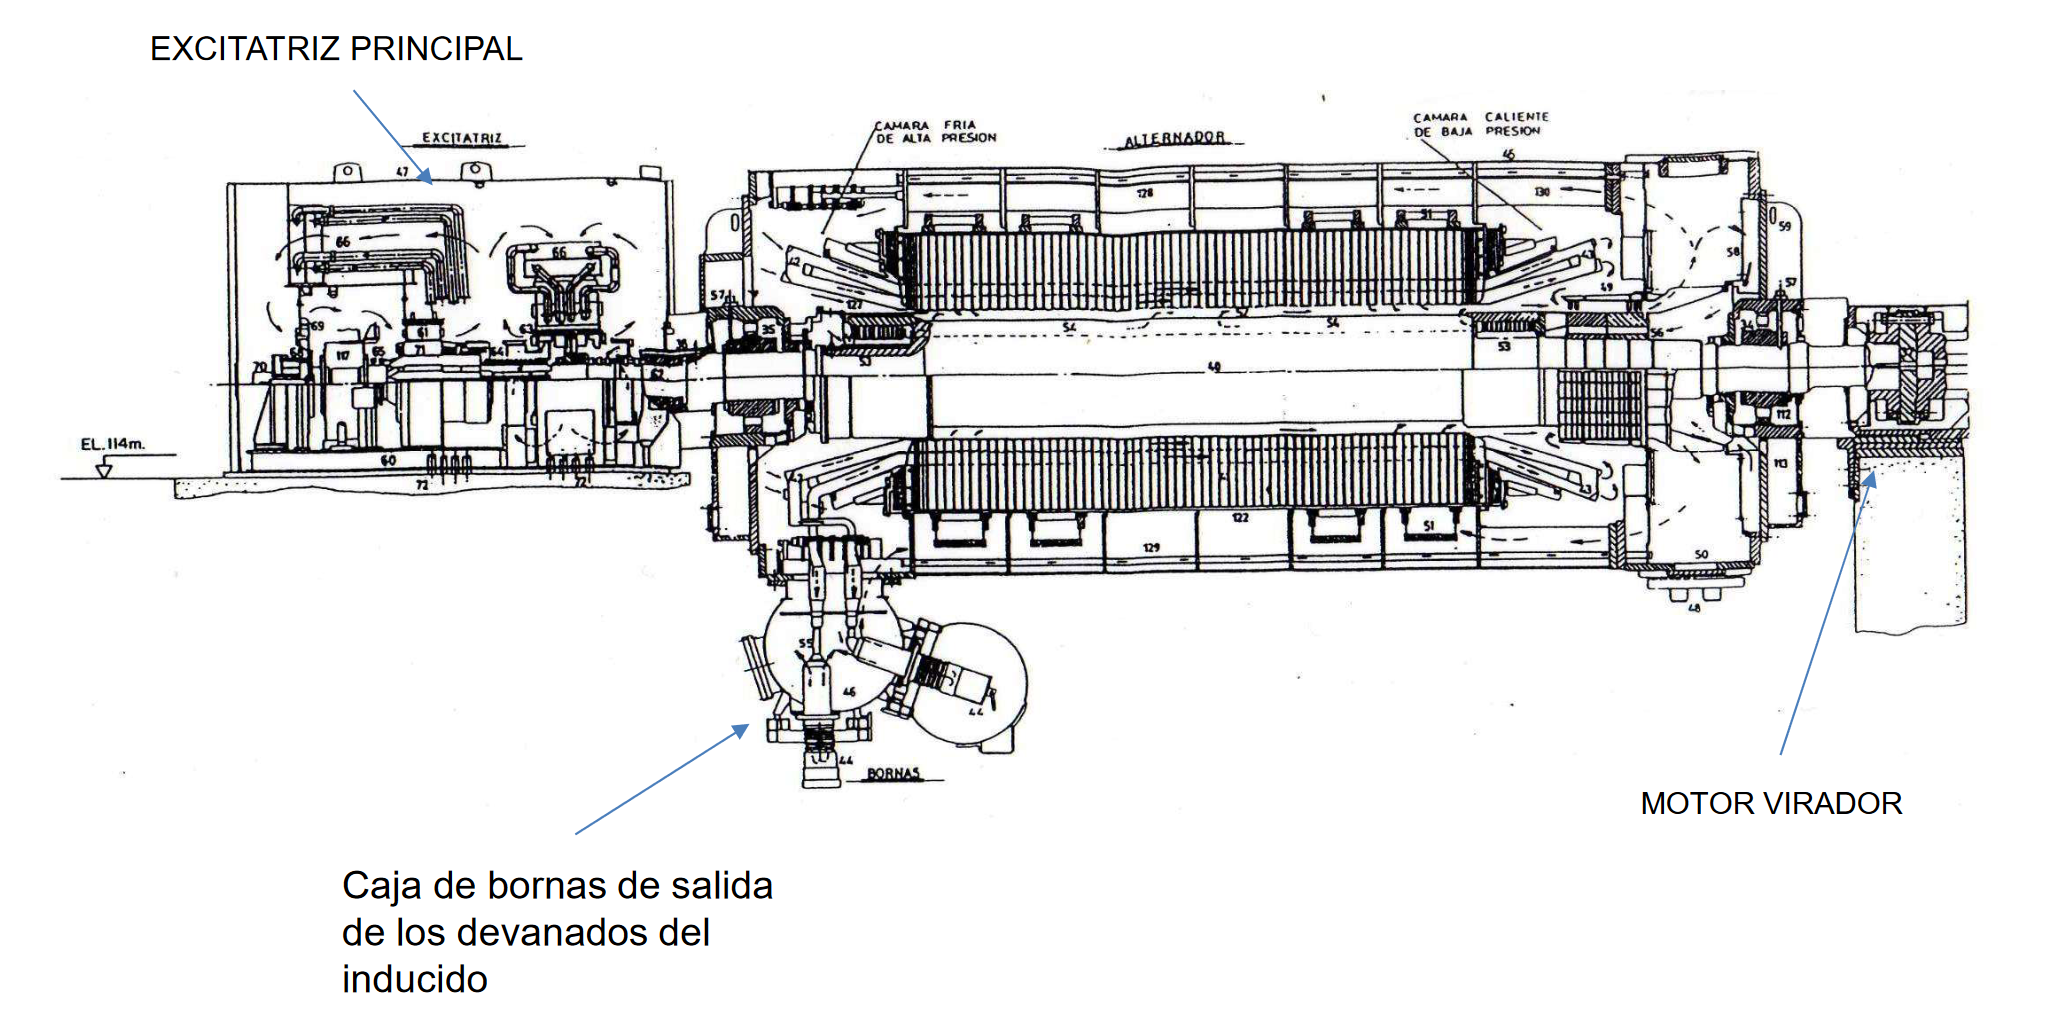
\includegraphics[width=0.9\linewidth]{res/tema6/generador}
			\label{fig:generador}
		\end{figure}
		
		\subsection{Conductores de salida del estátor. Barras de fase aislada.}
			Tienen una capacidad nominal de corriente desde 3 $kA$ hasta 50 $kA$. Se prolongan hasta el bloque interruptor automático + seccionador, bornes de baja tensión del transformador de potencia y el lado
			de alta tensión del transformador de servicios auxiliares. Por su interior circula aire o hidrógeno mediante ventiladores centrífugos. Consta de las siguientes partes:
			
			\begin{itemize}
				\item \textbf{Conductor:} tubo redondo de aluminio extruido de alta conductividad o barras de cobre.
				\item \textbf{Aisladores:} de porcelana o de resina epoxy. Sujetos rígidamente a los tubos de aluminio. Puede haber de uno a cuatro aisladores.
				\item \textbf{Tubo pantalla:} De aluminio. Su misión es doble: servir como conducto para la circulación del refrigerante (hidrógeno o aire) y como apantallamiento para el flujo creado por las altas intensidades. Se ponen a tierra por varios puntos.
			\end{itemize}
		
	\section{Circuito equivalente de un generador síncrono.}
		\subsection{Principio de funcionamiento.}
			En una máquina síncrona las tensiones inducidas forman un sistema trifásico equilibrado y de secuencia directa. Estas tensiones inducidas, si no se consideran efectos de saturación, son proporcionales a la intensidad de excitación en corriente continua, dado que la velocidad de rotación tiene que ser constante para mantener la frecuencia de la red constante.
			
			
			\begin{figure}[H]
				\begin{minipage}{0.5\textwidth}
					\begin{figure}[H]
						\centering
						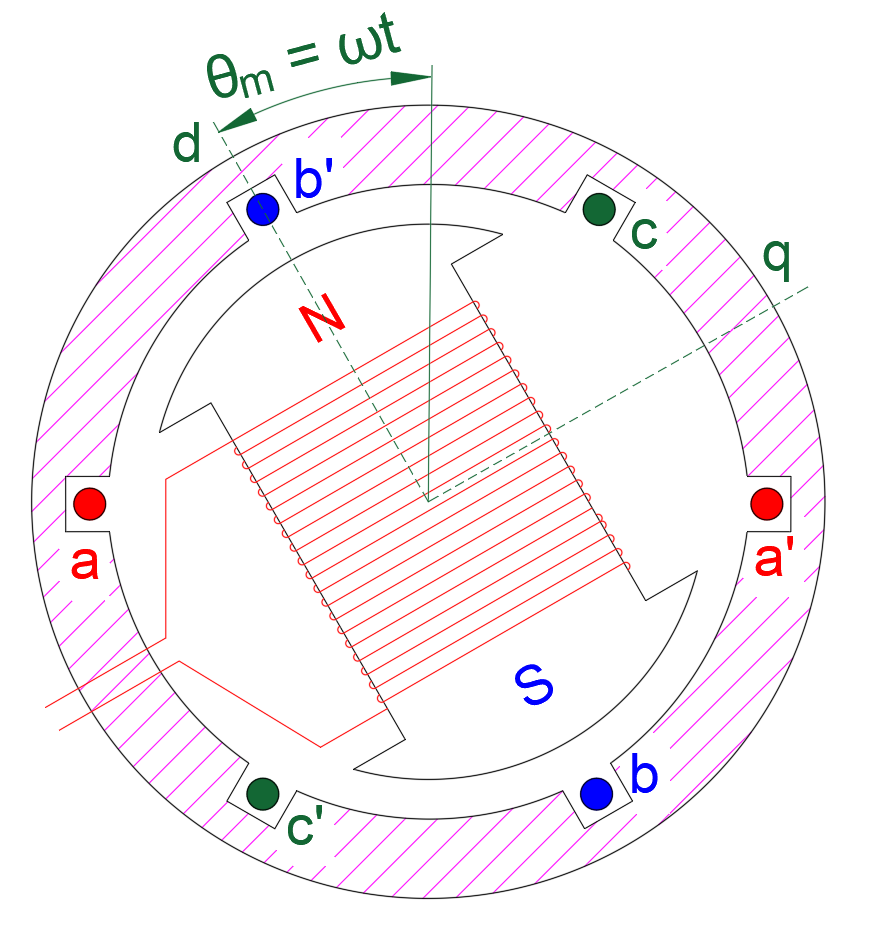
\includegraphics[width=0.7\linewidth]{res/tema6/ejes_dq}
						\label{fig:ejesdq}
					\end{figure}
				\end{minipage}
				\begin{minipage}{0.5\textwidth}
					Si el generador es de polos salientes la reluctancia en el entrehierro no es uniforme y aparecen dos reactancias:
					\begin{itemize}
						\item \textbf{Reactancia del eje directo:} $X_d$.
						\item \textbf{Reactancia del eje transversal o en cuadratura:} $X_q$.
					\end{itemize}
					Si el generador es de rotor cilíndrico sólo se considera la \textbf{reactancia síncrona:} $X_s$.
					
					\[f = \dfrac{p\cdot n}{60} \qquad E = k\cdot \omega \cdot i_{ex}\]
				\end{minipage}
			\end{figure}
			
		\subsection{Circuito equivalente por fase.}
			Considerando un generador de rotor cilíndrico o liso, al conectarla una carga y circular intensidad, estas corrientes crean un campo magnético, denominado \textbf{reacción de inducido}, que presenta una distribución senoidal y que gira a la misma velocidad y en el mismo sentido que el rotor. Esto provoca una caída de tensión en carga respecto de la tensión en vacío, y se representa mediante una reactancia de reacción de inducido, $X_{ri}$.
			
			\begin{figure}[H]
				\begin{minipage}{0.5\textwidth}
					\begin{figure}[H]
						\centering
						\begin{circuitikz}
							\tikzstyle{every node}=[font=\normalsize]
							\draw (3.25,18) to[sinusoidal voltage source, sources/symbol/rotate=auto,l={$\vec E_a$}] (3.25,14.75);
							\draw (3.25,18) to[L,l={$jX_{ri}$} ] (5,18);
							\draw (5,18) to[L,l={$jX_\sigma$} ] (6.75,18);
							\draw (6.75,18) to[R,l={$R$}] (8.5,18);
							\draw [](8.5,18) to[short, -o] (9,18) ;
							\draw [](3.25,14.75) to[short, -o] (9,14.75);
							\draw [->, >=Stealth] (9,17.5) -- (9,15.25)node[pos=0.5,right]{$\vec U_a$};
							\draw [short] (3.5,19) -- (6.5,19)node[pos=0.5,above]{$jX_s$};
							\draw [short] (3.5,19) -- (3.5,18.75);
							\draw [short] (6.5,19) -- (6.5,18.75);
							\draw [->, >=Stealth] (8.25,18) -- (8.75,18)node[pos=0.7,above]{$\vec I_a$};
							\draw [->, >=Stealth] (5,17.5) -- (5,15.25)node[pos=0.5,right]{$\vec E_{ag}$};
						\end{circuitikz}
					\end{figure}
				\end{minipage}
				\begin{minipage}{0.5\textwidth}
					No todo el flujo que crea el inductor es recogido por el inducido. Esta pérdida de flujo se representa mediante una reactancia de dispersión $X_\sigma$.
					
					\[\vec U_a = \vec E_a - \vec I_a(R + jX_{ri} + jX_{\sigma})\]
					\[\Downarrow\]
					\[\vec U_a = \vec E_a - \vec I_a(R + jX_s)\]
					\[\vec U_a = U_a\phase{0^\circ} \qquad \vec E_a = E_a\phase{\delta}\]
				\end{minipage}
			\end{figure}
			
			\begin{figure}[H]
				\begin{minipage}{0.3\textwidth}
					Considerando $R\approx 0$:
					\[P_G = \dfrac{E_a\cdot U_a}{X_S}\cdot \sin \delta\]
					\[Q_G = \dfrac{E_a\cdot U_a \cdot \cos \delta - U_a^2}{X_S}\]
				\end{minipage}
				\begin{minipage}{0.7\textwidth}
					\begin{figure}[H]
						\centering
						\begin{circuitikz}
							\tikzstyle{every node}=[font=\normalsize]
							\draw [ color={rgb,255:red,0; green,0; blue,255}, ->, >=Stealth] (5,14.75) -- (7.75,14.75)node[pos=1,above]{$\vec{U}$};
							\draw [ color={rgb,255:red,255; green,0; blue,0}, ->, >=Stealth] (7.75,14.75) -- (8.5,14)node[pos=1,below]{$R\vec{I}$};
							\draw [ color={rgb,255:red,255; green,0; blue,0}, ->, >=Stealth] (8.5,14) -- (10.5,16.25)node[pos=0.5,right]{$jX_\sigma\vec{I}$};
							\draw [ color={rgb,255:red,0; green,128; blue,0}, ->, >=Stealth] (5,14.75) -- (10.5,16.25)node[pos=0.9,above]{$\vec{E}_{ag}$};
							\draw [ color={rgb,255:red,128; green,0; blue,255}, ->, >=Stealth] (5,14.75) -- (6.25,13.5)node[pos=1,below]{$\vec{I}$};
							\draw [ color={rgb,255:red,210; green,105; blue,0}, ->, >=Stealth] (5,14.75) -- (4,17.75)node[pos=1,right]{$\Phi$};
							\draw [ color={rgb,255:red,255; green,128; blue,0}, ->, >=Stealth] (5,14.75) -- (4.25,17)node[pos=1,right]{$\vec{F}_{r}$};
							\draw [ color={rgb,255:red,255; green,0; blue,128}, ->, >=Stealth] (4.25,17) -- (3,18.25)node[pos=0.8,above]{$\,\,\,\,\vec{F}_i$};
							\draw [ color={rgb,255:red,0; green,128; blue,128}, ->, >=Stealth] (5,14.75) -- (11.75,17.75)node[pos=0.9,above]{$\vec{E}_a$};
							\draw [ color={rgb,255:red,255; green,0; blue,0}, ->, >=Stealth] (10.5,16.25) -- (11.75,17.75)node[pos=0.5,right]{$jX_r\vec{I}$};
							\draw [ color={rgb,255:red,128; green,128; blue,128}, ->, >=Stealth] (5,14.75) -- (2.57,19)node[pos=1,left]{$\Phi_0$};
							\draw [->, >=Stealth] (5,14.75) -- (3,18.25)node[pos=0.9,left]{$\vec{F}_{ex}$};
							\draw (6,14.75) arc [radius=1cm, start angle=0, end angle=-45]node[pos=0.6,right]{$\varphi$};
							\draw (6.5,14.75) arc [radius=1.5cm, start angle=0, end angle=25]node[pos=0.4,right]{$\delta$};
							\draw (7,15.275) arc [radius=2cm, start angle=10, end angle=19]node[pos=0.9,right]{$\delta_m$};
						\end{circuitikz}
					\end{figure}
				\end{minipage}
			\end{figure}
			
			\begin{figure}[H]
				\begin{minipage}{0.65\textwidth}
					\begin{figure}[H]
						\centering
						\begin{circuitikz}[scale = 0.9]
							\tikzstyle{every node}=[font=\normalsize]
							\draw [ color={rgb,255:red,255; green,0; blue,0}, ->, >=Stealth] (10.25,12) -- (14.25,12)node[pos=0.6,below]{$\dfrac{3U_a^2}{X_S}$};
							\draw [->, >=Stealth] (14.25,12) -- (14.25,16.25)node[pos=1,above]{$P\,[MW]$};
							\draw [->, >=Stealth] (14.25,12) -- (17,12)node[pos=1,right]{$Q\,[MV\!A]$};
							\draw [ color={rgb,255:red,0; green,128; blue,255}, ->, >=Stealth] (14.25,12) -- (15.5,14.5)node[pos=0.5,left]{S};
							\draw [ color={rgb,255:red,0; green,128; blue,0}, ->, >=Stealth] (10.25,12) -- (15.5,14.5)node[pos=0.5,above]{$\dfrac{3U_a}{X_S}\cdot E_a$};
							\node [font=\normalsize] at (14.5,11.75) {O};
							\node [font=\normalsize] at (10,11.75) {M};
							\node [font=\normalsize] at (15.25,14.75) {B};
							\node [font=\normalsize] at (15.75,12.25) {A};
							\draw [dashed] (15.5,14.5) -- (15.5,12);
							\draw [dashed] (15.5,14.5) -- (16,15.5);
							\draw [<->, >=Stealth] (14.25,15.25) .. controls (15,15.5) and (15.4,15.25) .. (15.75,15)node[pos=0.5,above]{$\phi$};
							\draw [<->, >=Stealth] (12.75,13.2) .. controls (13,12.75) and (13.1,12.5) .. (13,12)node[pos=0.5,right]{$\delta$};
							\draw [<->, >=Stealth] (16.25,14.5) -- (16.25,12)node[pos=0.5,right]{$P$};
							\draw [short] (15.5,14.5) -- (16.5,14.5);
							\draw [<->, >=Stealth] (14.25,11.25) -- (15.5,11.25)node[pos=0.5,below]{$Q$};
							\draw [ color={rgb,255:red,0; green,128; blue,255}, dashed] (14.25,12) -- (13.25,10.25);
							\draw [ color={rgb,255:red,255; green,128; blue,0}, ->, >=Stealth] (10.25,12) -- (13.25,10.25)node[pos=0.5,below, sloped]{$\dfrac{U_a}{X_S}\cdot I_a$};
							\draw [short] (14.25,11) -- (14.25,12);
							\draw [short] (15.5,11) -- (15.5,12);
							\node at (10.25,12) [circ] {};
							\node at (14.25,12) [circ] {};
							\node at (15.5,14.5) [circ] {};
							\node at (15.5,12) [circ] {};
						\end{circuitikz}
						
						\label{fig:my_label}
					\end{figure}
				\end{minipage}
				\begin{minipage}{0.35\textwidth}
					Se pueden obtener los valores de P y Q multiplicando escalarmente todos los vectores por $\dfrac{U_a}{X_S}$, si consideramos despreciable la $R$. Será útil a la hora de dibujar el diagrama de capacidad de la máquina.
					\[P = 3\cdot U_a \cdot I_a \cdot \cos \phi\]
					\[Q = 3\cdot U_a \cdot I_a \cdot \sin \phi\]
				\end{minipage}
			\end{figure}
			
		\subsection{Modelo fasorial para un generador de polos salientes.}
			\begin{figure}[H]
				\centering
					\begin{circuitikz}
						\tikzstyle{every node}=[font=\normalsize]
						\draw [ color={rgb,255:red,255; green,0; blue,0}, ->, >=Stealth] (10.25,12) -- (16,12)node[pos=0.85,below]{$\vec U_a$};
						\draw [ color={rgb,255:red,0; green,128; blue,0}, ->, >=Stealth] (10.25,12) -- (19.25,13.5)node[pos=0.5,above]{$\vec{E}_a$};
						\node [font=\normalsize] at (10,12.25) {O};
						\draw [<->, >=Stealth] (14.75,12.75) .. controls (14.85,12.5) and (14.85,12.25) .. (14.75,12)node[pos=0.5,right]{$\delta$};
						\node at (10.25,12) [circ] {};
						\draw [ color={rgb,255:red,255; green,128; blue,0}, ->, >=Stealth] (16,12) -- (16.75,11.5)node[pos=0.5,above, sloped]{$R\vec I_a$};
						\draw [<->, >=Stealth] (12.75,12) .. controls (12.75,11.5) and (12.75,11.25) .. (12.5,10.75)node[pos=0.5,right]{$\varphi$};						
						\draw [ color={rgb,255:red,0; green,128; blue,255}, ->, >=Stealth] (10.25,12) -- (10.75,9.75)node[pos=0.5,right]{$\vec I_{ad}$};
						\draw [ color={rgb,255:red,0; green,128; blue,255}, ->, >=Stealth] (10.25,12) -- (13,12.45)node[pos=0.5,above, sloped]{$\vec I_{aq}$};
						\draw [dashed] (13,12.45) -- (13.5,10.25);
						\draw [dashed] (10.75,9.75) -- (13.5,10.25);
						\draw [ color={rgb,255:red,0; green,128; blue,255}, ->, >=Stealth] (19.5,12) -- (19.25,13.5)node[pos=0.5,right]{$jX_q \vec I_{aq}$};
						\draw [ color={rgb,255:red,0; green,128; blue,255}, ->, >=Stealth] (16.75,11.5) -- (19.5,12)node[pos=0.5,above, sloped]{$jX_d \vec I_{ad}$};
						\draw [ color={rgb,255:red,255; green,128; blue,0}, ->, >=Stealth] (10.25,12) -- (13.5,10.25)node[pos=0.5,above]{$\vec I_a$};
						\draw [ color={rgb,255:red,0; green,128; blue,255}, dashed] (10.25,12) -- (9.75,14.25)node[pos=1,right]{d};
						\draw [ color={rgb,255:red,0; green,128; blue,255}, dashed] (19.25,13.5) -- (20.75,13.75)node[pos=1,above]{q};
					\end{circuitikz}
				
				\label{fig:my_label}
			\end{figure}
			
			Recordar que $d \perp q$. Se suele considerar $X_S = \dfrac{X_d + X_q}{2}$
			\[\vec U_a = \vec E_a - R\vec I_a - jX_d \vec I_{ad} - jX_q \vec I_{aq} \quad \Rightarrow \quad \vec U_a = \vec E_a - R\vec I_a - j(X_d - X_q)\vec I_{ad} - jX_q \vec I_a\]
			
			
			El vector $j(X_d - X_q)\vec I_{ad}$ está en fase con $\vec E_a$.
			
			\[P_G = \dfrac{U_a E_a}{X_d} \sen \delta + \dfrac{U_a^2}{2}\left(\dfrac{1}{X_q} - \dfrac{1}{X_d}\right)\sin 2\delta\]
			\[Q_G = \dfrac{U_a E_a}{X_d} \cos \delta - U_a^2\left(\dfrac{\sin^2 \delta}{X_q} + \dfrac{\cos^2 \delta}{X_d}\right)\]
			
		\subsection{Determinación de la reactancia síncrona saturada.}
			Se obtiene a través de ensayos de vacío y cortocircuito, utilizando sus curvas características. La impedancia saturada da resultados más precisos que la no saturada.
			\[Z_{s0} = f(E_0)\equiv f(I_e) \quad \because E_0 = f(I_e)\]
			\[Z_{s0} = \dfrac{U_N}{I_{cc0}}\qquad X_S = \sqrt{Z_S^2 - R^2}\]
			
		\subsection{Estabilidad.}
		\vspace{-1.5cm}
			\begin{figure}[H]
				\begin{minipage}{0.5\textwidth}
					\begin{figure}[H]
						\centering
						\begin{circuitikz}[scale = 1.1]
							\tikzstyle{every node}=[font=\normalsize]
							\draw [->, >=Stealth] (11,11.75) -- (15.75,11.75)node[pos=1,right]{$\delta$};
							\draw [->, >=Stealth] (11,11.75) -- (11,16)node[pos=1,right]{P};
							\draw [color={rgb,255:red,255; green,0; blue,0},short] (11,11.75) .. controls (12.75,17.25) and (13.5,17) .. (15.25,11.75);
							\node [font=\normalsize] at (15.25,11.5) {$180^\circ$};
							\draw [dashed] (11,14.75) -- (15.5,14.75)node[pos=0,left]{$P_m$};
							\draw [dashed] (11,13.25) -- (15.5,13.25)node[pos=0,left]{$P_0$};
							\draw [short] (11.5,13.25) -- (11.5,14.75);
							\draw [short] (11.5,14.75) -- (12.75,14.75);
							\draw [short] (12.75,14.75) -- (12.75,15.65);
							\node [font=\normalsize] at (11.75,14.5) {A1};
							\node [font=\normalsize] at (12.5,15) {A2};
							\draw [dashed] (11.5,13.25) -- (11.5,11.75)node[pos=1,below]{$\delta_{0}$};
							\draw [dashed] (12.75,14.75) -- (12.75,11.75)node[pos=1,below]{$\delta_{max}$};
							\draw [dashed] (12.125,14.75) -- (12.125,11.75)node[pos=1,below]{$\delta_m$};
						\end{circuitikz}
						
						\label{fig:my_label}
					\end{figure}
				\end{minipage}
				\begin{minipage}{0.5\textwidth}
					Límite de estabilidad: $\delta = 90^\circ$.
					
					
					\textbf{Estabilidad transitoria:} Ante un cambio del ángulo del par provocado por un cambio brusco de potencia activa en la red, se produce un proceso oscilante de aceleración y deceleración, que se va amortiguando en un tiempo que depende de la inercia de las masas en rotación de la unidad de generación, turbina y generador. Durante este proceso, el generador pierde la sincronización con la red y aparecen sobreintensidades en las líneas.
				\end{minipage}
			\end{figure}
			
			Si las áreas formadas de aceleración (A1) y deceleración (A2) son iguales se consigue la estabilización en un nuevo valor de ángulo y P. En caso contrario, el sistema se vuelve inestable y hay que desacoplar el generador de la red.
			
		\subsection{Comportamiento conectado a la red eléctrica.}
			\vspace{-0.5cm}
			\begin{figure}[H]
				\begin{minipage}{0.5\textwidth}
					Se supone que la potencia nominal de la máquina es pequeña con relación al resto del sistema. A este nudo se le denomina nudo de potencia infinita. Se consideran $X_S$ de la máquina y $U_{red}$ constantes.
				\end{minipage}
				\begin{minipage}{0.5\textwidth}
					\begin{figure}[H]
						\centering
						\begin{circuitikz}
							\tikzstyle{every node}=[font=\normalsize]
							\draw (11.5,14) to[sinusoidal voltage source, sources/symbol/rotate=auto,l={ \normalsize $\vec U_p$}] (11.5,12);
							\draw (11.5,14) to[L,l={ \normalsize $X_S$} ] (14.25,14);
							\draw (14.25,14) to[sinusoidal voltage source, sources/symbol/rotate=auto,l={ \normalsize $\vec U_{red}$}] (14.25,12);
							\draw (11.5,12) to (11.5,11.75) node[ground]{};
							\draw (14.25,12) to (14.25,11.75) node[ground]{};
							\draw [->, >=Stealth] (13.5,14) -- (14,14)node[pos=0.5,above]{$\vec I_p$};
						\end{circuitikz}
						
						\label{fig:my_label}
					\end{figure}
				\end{minipage}
			\end{figure}
			
	\section{Diagrama límite de capacidad de la máquina síncrona.}
		El campo de funcionamiento posible de la máquina cuando está acoplada a una red de potencia infinita queda limitado por los siguientes límites:
		\begin{itemize}
			\item \textbf{Límite térmico del inducido:} $I_{max}$. La corriente máxima que el inducido puede dar teniendo en cuenta su calentamiento admisible. Si se considera la tensión en bornes constante el límite térmico se puede establecer como una $S_{max}$.
			
			\item \textbf{Límite de tensión interna máxima:} $E_{max}$. Definida por la intensidad máxima de excitación que puede recorrer el rotor y/o la máxima tensión de aislamiento. Suele ser $2.1 p.u.$
			
			\item \textbf{Límites de la potencia mecánica:} $P_{max},\,P_{min}$. Establecidas por las potencias máxima y mínima que puede dar/necesita la turbina.
			
			\item \textbf{Límite de estabilidad:} $\delta_{max}$. Se establece a partir del apartado anterior. El $\delta_{max}$ práctico suele estar en torno a $80^\circ$.
		\end{itemize}
			
		\begin{figure}[H]
			\centering
			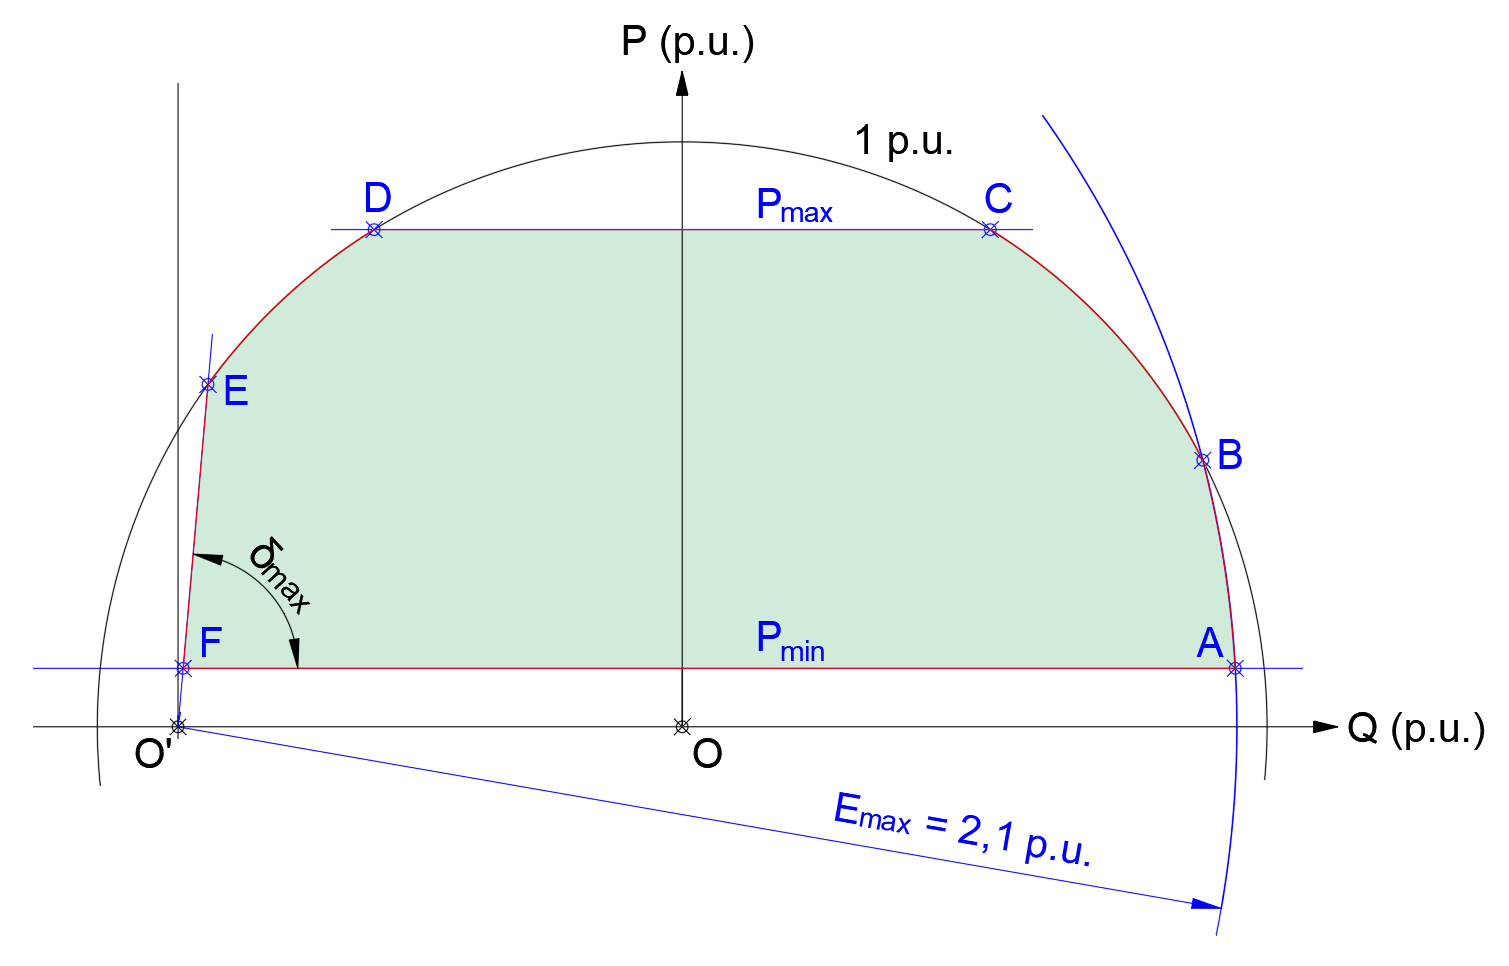
\includegraphics[width=0.8\linewidth]{res/tema6/diagramaCapacidad}
			\label{fig:diagramacapacidad}
		\end{figure}
		
	\section{Modos de funcionamiento de una máquina síncrona.}
		\begin{table}[H]
			\centering
			\renewcommand{\arraystretch}{1.1}
			\begin{tabular}{ccccl}
				\textbf{Caso} & \textbf{Finalidad} & \textbf{Constantes} & \textbf{Variables} & \textbf{Consecuencias}\\
				\hline
				\multirow{3}{*}{1} & \multirow{3}{*}{Variar $P$}   & \multirow{3}{*}{$I_{ex}$}  & \multirow{3}{*}{$P_{mec}$}  & $\Phi = cte \Rightarrow E_0 = cte \Rightarrow n = cte$ \\
				&              &           &            & $\updownarrow\delta\Rightarrow\updownarrow jX_S\vec{I}_a\Rightarrow\updownarrow P_a$ \\
				&              &           &            & $\uparrow\delta \Rightarrow\uparrow P\text{ y }\downarrow Q$ \\\hline
				\multirow{6}{*}{2} & \multirow{6}{*}{Variar $Q$}   & \multirow{6}{*}{$P_{mec}$} & \multirow{6}{*}{$I_{ex}$}   & $\updownarrow E_a$ \\
				&              &           &            & $Proy_P(jX_s\vec{I}_a) = cte$ \\
				&              &           &            & $Proy_Q(jX_s\vec{I}_a)$: \\
				&              &           &            & $\quad\text{Sobreexcitada, inductivo}$ \\
				&              &           &            & $\quad\text{Subexcitada, capacitivo}$ \\
				&              &           &            & $\quad\cos{\varphi} = 1$ \\\hline
				\multirow{3}{*}{3} & \multirow{3}{*}{Asincronismo} & \multirow{3}{*}{$P_{mec}$} & \multirow{3}{*}{$I_{ex}$}   & La red aporta la magnetización de la máquina $\Rightarrow$ \\
				&              &           &            & sobreintensidades en el inducido. \\
				&              &           &            & Aporta $P$, consume $Q$ \\\hline
				\multirow{3}{*}{4} & \multirow{3}{*}{\parbox{2cm}{\centering Oscilaciones\\pendulares}} & \multirow{3}{*}{$I_{ex}$}  & \multirow{3}{*}{\parbox{2cm}{\centering C. bruscos\\$P_{mec}$}} & Pérdida de la sicronización con la red. \\
				&              &           &   & Sobreintensidades en las líneas. \\
				&              &           &            & \textuparrow Inercia \textrightarrow \textuparrow Tiempo de oscilación\\\hline
				\multirow{2}{*}{5} & Compensador  & \multirow{2}{*}{$I_{ex}$}  & \multirow{2}{*}{$P_{mec}$}  & Consumo de $P_{mec}$ por pérdida de par en el eje. \\
				& síncrono     & 			 & 			  & Consume activa, consume o aporta reactiva.\\\hline
			\end{tabular}
			\label{tab:modosFunc}
		\end{table}
		
		\begin{figure}[H]
			\begin{minipage}{0.5\textwidth}
				\begin{figure}[H]
					\centering
					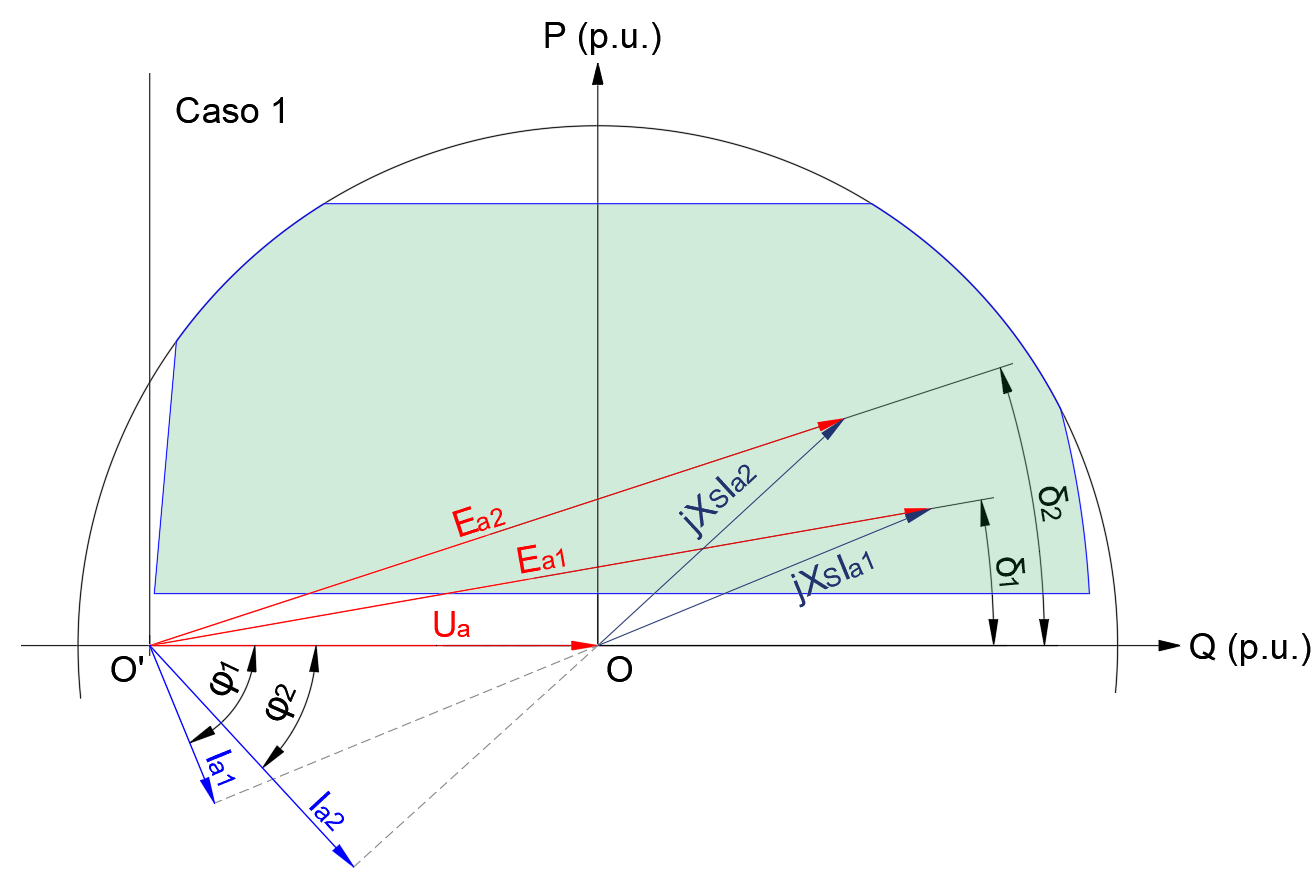
\includegraphics[width=1\linewidth]{res/tema6/modoFunc1}
					\label{fig:modofunc1}
				\end{figure}
			\end{minipage}
			\begin{minipage}{0.5\textwidth}
				\begin{figure}[H]
					\centering
					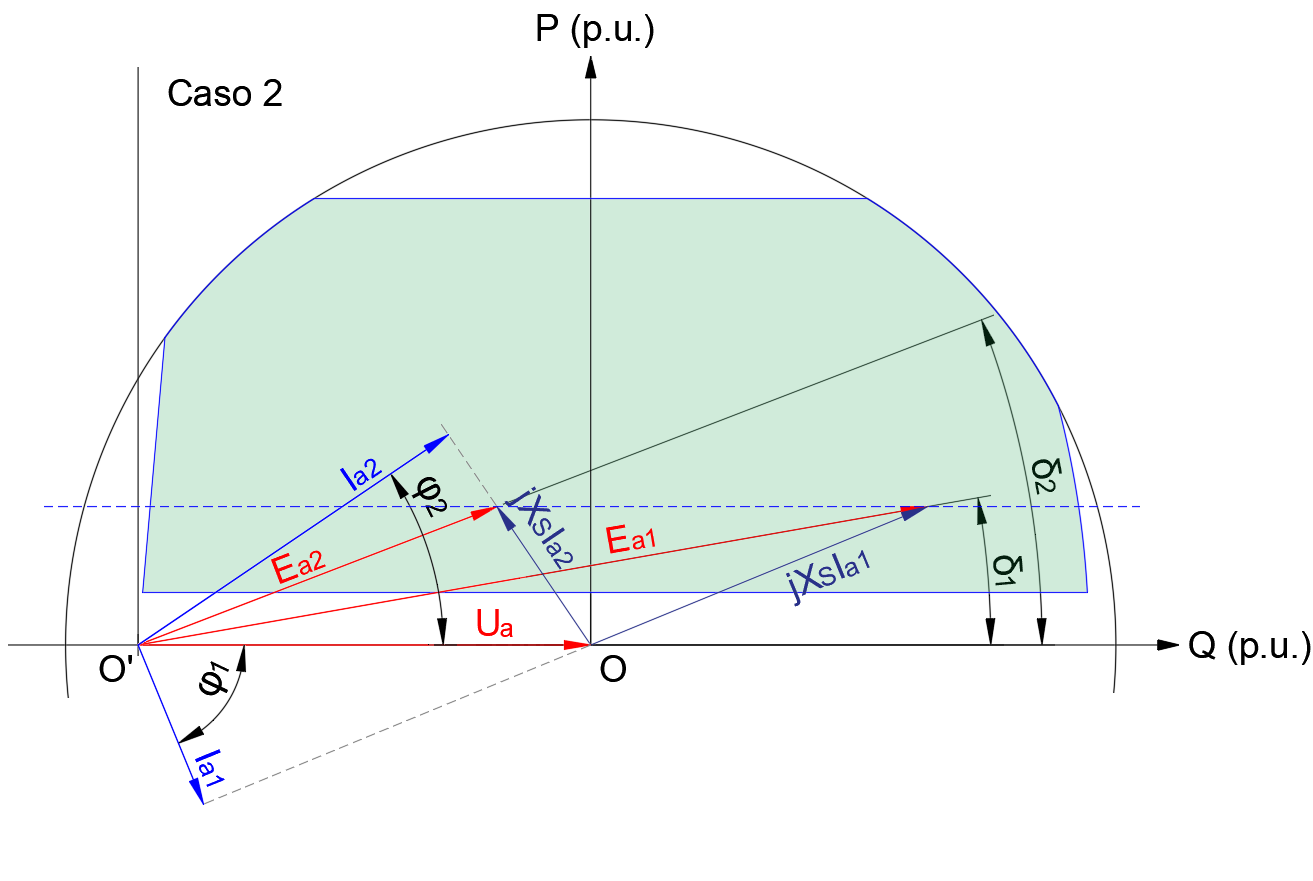
\includegraphics[width=1\linewidth]{res/tema6/modoFunc2}
					\label{fig:modofunc2}
				\end{figure}
			\end{minipage}
		\end{figure}
		
		
	\section{Ejercicio completo resuelto.}		
		Un alternador de polos salientes de una central hidráulica tiene las siguientes características técnicas:
		\begin{figure}[H]
			\begin{minipage}{0.33\textwidth}
				\begin{itemize}
					\item $S_n = 300\,MV\!A$
					\item $U_n = 22\,kV$
					\item $\cos \varphi_n = 0.85\,ind$
					\item $p = 20$
				\end{itemize}
			\end{minipage}
			\begin{minipage}{0.33\textwidth}
				\begin{itemize}
					\item $\delta_{max} = 85^\circ$
					\item $X_d = 2.45\,\varOmega/fase$
					\item $X_q = 1.45\,\varOmega/fase$
				\end{itemize}
			\end{minipage}
			\begin{minipage}{0.33\textwidth}
				\begin{itemize}
					\item $E_{\text{\textit{exc, máx}}} = 2.1\,p.u.$
					\item $P_{max} = 255\,MW$
					\item $P_{min} = 45\,MW$
				\end{itemize}
			\end{minipage}
		\end{figure}
		

		Dibujar el diagrama de capacidad en valores $p.u.$ y calcular los valores de $P\,[MW]$, $Q\,[MV\!Ar]$, $S\,[MV\!A]$, $I\,[kA]$, $\cos \varphi$, $E\,[kV]$ y $\delta$ para cada punto de intersección entre valores límites. Considerar despresciable la caída de tensión en los devanados del inducido por la resistencia 
		interna.
		
		
		\noindent\makebox[\linewidth]{\rule{\paperwidth}{0.4pt}}
		\vspace{-0.2cm}
		
		
		$S_n = S_b = 1\,p.u.\qquad U_n = U_b = 1\,p.u.$
		
		\vspace{0.1cm}
		$I_n = \dfrac{S_b}{\sqrt{3}U_b} = \dfrac{300\cdot 10^6}{\sqrt{3}\cdot 22\cdot 10^3} = 7.87\,kA = I_b$
		
		\vspace{0.1cm}
		$Z_b = \dfrac{U_b^2}{S_b} = \dfrac{(22\cdot 10^3)^2}{300\cdot 10^6} = 1.61\,\varOmega$
		
		\vspace{0.1cm}
		$X_s = \dfrac{X_d + X_q}{2} = \dfrac{2.45 + 1.45}{2} = 1.95\,\varOmega/fase\quad \Rightarrow \quad X_{s,\,p.u.} = \dfrac{X_s}{Z_b} = 1.21\,p.u.$
		
		\vspace{0.1cm}
		Límite inductor $=\dfrac{E\cdot U_n}{X_{s,\,p.u.}} = \dfrac{2.1\cdot 1}{1.21} = 1.7355\,p.u.$
		
		\vspace{0.1cm}
		$P_{max,\,p.u.} = \dfrac{255}{300} = 0.85\,p.u.\qquad P_{min,\,p.u.} = \dfrac{45}{300} = 0.15\,p.u.$
		
		\subsubsection*{Punto A.}
			Datos conocidos: $P_{min} = 0.15\,p.u.\quad E_{max} = 2.1\,p.u.\quad X_s = 1.21\,p.u.\quad U = 1\,p.u.$
			
			\vspace{0.1cm}
			$P_A = \dfrac{E\cdot U}{X_s}\cdot \sin \delta = 0.15 \quad \Rightarrow \quad \delta = 4.95^\circ$
			
			\vspace{0.1cm}
			$Q_A = \dfrac{E\cdot U}{X_s}\cdot \cos \delta - \dfrac{U^2}{X_s} = 0.9\,p.u.\cdot S_b = 271.08\,MV\!Ar$
			
			\vspace{0.1cm}
			$S_A = \sqrt{P_A^2+Q_A^2} = 0.92\cdot S_b = 276\,MV\!A$
			
			\vspace{0.1cm}
			$I_A = \dfrac{S_A}{\sqrt{3}\cdot U_A} = \dfrac{276\cdot 10^6}{\sqrt{3}\cdot 22\cdot 10^3} = 7.2\,kA$
			
			\vspace{0.1cm}
			$\varphi_A = \arctan \left(\dfrac{Q_A}{P_A}\right) = 80.57^\circ \quad \Rightarrow \quad \cos \varphi_A = 0.16$
		
		\subsubsection*{Punto B.}
			Datos conocidos: $S_n = 1\,p.u.\quad U_n = 1\,p.u.\quad X_s = 1.21\,p.u.\quad E_{max} = 2.1\,p.u.$
			
			\vspace{0.1cm}
			$
			\left.
			\begin{matrix}
				P_B = \dfrac{E_0\cdot U}{X_s}\cdot \sin \delta\\
				Q_B = \dfrac{E_0\cdot U}{X_s}\cdot \cos \delta - \dfrac{U^2}{X_s}\\\\
				S^2 = P^2 + Q^2
			\end{matrix}
			\right\}
			\left(\dfrac{E_0\cdot U}{X_s}\sin \delta\right)^2 + \left(\dfrac{E_0\cdot U}{X_s}\cos \delta - \dfrac{U^2}{X_s}\right)^2 = 1
			$
			
			\vspace{0.1cm}
			Resolviendo se obtiene $\cos \delta = 0.93 \quad \Rightarrow \quad \delta_B = 20^\circ$
			
			\vspace{0.1cm}
			$P_B = \dfrac{2.1\cdot 1}{1.21}\sin 20^\circ = 0.59\,p.u. \cdot S_b = 177.45\,MW$
			
			\vspace{0.1cm}
			$Q_B = \dfrac{2.1\cdot 1}{1.21}\cos 20^\circ - \dfrac{1^2}{1.21} = 0.81\,p.u.\cdot S_b = 241.89\,MV\!Ar$
			
			\vspace{0.1cm}
			$\varphi_B = \arctan\left(\dfrac{Q_B}{P_D}\right) = 53.74^\circ \quad \Rightarrow \quad \cos \varphi_B = 0.59$
			
			\vspace{0.1cm}
			$I_B = I_n = 7.87\,kA$
			
		\subsubsection*{Punto C.}
			Datos conocidos: $P_{max} = 0.85\,p.u.\quad S_n = 1\,p.u.\quad I_n = 7.87\,kA$
			
			\vspace{0.1cm}
			$Q_C = \sqrt{S^2 - P^2} = \sqrt{1^2 - 0.85^2} = 0.527\,p.u. = 158.03\,MV\!A$
			
			\vspace{0.1cm}
			$\tan \varphi_C = \dfrac{Q_C}{P_C} = \dfrac{158.03}{255} = 0.619 \quad \Rightarrow \quad \varphi_C = 31.78^\circ \quad \Rightarrow \quad \cos \varphi_C = 0.85$
			
			\vspace{0.1cm}
			$P_C = \dfrac{E_0\cdot U}{X_s}\sin \delta = 0.85\,p.u. \quad \Rightarrow \quad E_C = \dfrac{P_C \cdot X_S}{U\cdot \sin \delta}$
			
			\vspace{0.1cm}
			Sustituyendo en $Q_C = \dfrac{E_0\cdot U}{X_s}\cdot \cos \delta - \dfrac{U^2}{X_s} = \dfrac{\dfrac{P_C\cdot X_s}{U\cdot \sin \delta}}{X_s}\cos \delta - \dfrac{U^2}{X_s} = \dfrac{P_C}{\sin \delta}\cos \delta - \dfrac{U^2}{X_s} = 0.527$
			
			\vspace{0.1cm}
			$\dfrac{0.85}{\sin \delta}\cos \delta - \dfrac{1}{1.21} = 0.527 \quad \Rightarrow \quad \dfrac{0.85}{\tan \delta} = 1.350 \quad \Rightarrow \quad \tan \delta = 0.628 \quad \Rightarrow \quad \delta_C = 32.129^\circ$
			
			\vspace{0.1cm}
			$E_C = \dfrac{0.85\cdot 1.21}{1\cdot \sin 32.12^\circ} = 1.933\,p.u. = 42.54\,kV$
			
		\subsubsection*{Punto D.}
			Datos conocidos: $P_{max} = 0.85\,p.u.\quad S_n = 1\,p.u.\quad I_n = 7.87\,kA$
			
			\vspace{0.1cm}
			$Q_D = \sqrt{S^2 - P^2} = -0.527 = -158.03\,MV\!Ar$
			
			\vspace{0.1cm}
			$\tan \varphi_D = \dfrac{Q_D}{P_D} = \dfrac{-158.03\,MV\!Ar}{255\,MW} = -0.619 \quad \Rightarrow \quad \varphi_D = -31.78^\circ \quad \Rightarrow \quad \cos \varphi_D = 0.85$ (cap)
			
			\vspace{0.1cm}
			$P_D = \dfrac{E_0\cdot U}{X_s}\sin \delta = 0.85\,p.u. \quad \Rightarrow \quad E_D = \dfrac{P_D \cdot X_s}{U\cdot \sin \delta}$
			
			\vspace{0.1cm}
			Sustituyendo en $Q_D = \dfrac{E_0\cdot U}{X_s}\cdot \cos \delta - \dfrac{U^2}{X_s} = \dfrac{\dfrac{P_C\cdot X_s}{U\cdot \sin \delta}}{X_s}\cos \delta - \dfrac{U^2}{X_s} = \dfrac{P_D}{\sin \delta}\cos \delta - \dfrac{U^2}{X_s} = -0.527$
			
			\vspace{0.1cm}
			Operando se obtiene $\tan \delta = 2.83 \quad \Rightarrow \quad \delta = 70.59^\circ$
			
			\vspace{0.1cm}
			$E_D = \dfrac{0.85\cdot 1.21}{1\cdot \sin 70.59^\circ} = 1.09 = 23.99\,kV$
		
		\subsubsection*{Punto E.}
			Datos conocidos: $S_n = 1\,p.u.\quad I_n = 7.87\,kA\quad \delta_{max} = 85^\circ$
			
			\vspace{0.1cm}
			$
			\left.
			\begin{matrix}
				P_E = \dfrac{E_0\cdot U}{X_s}\cdot \sin \delta\\
				Q_E = \dfrac{E_0\cdot U}{X_s}\cdot \cos \delta - \dfrac{U^2}{X_s}\\\\
				S^2 = P^2 + Q^2
			\end{matrix}
			\right\}
			\left(\dfrac{E_0\cdot U}{X_s}\sin \delta\right)^2 + \left(\dfrac{E_0\cdot U}{X_s}\cos \delta - \dfrac{U^2}{X_s}\right)^2 = 1
			$
			
			\vspace{0.1cm}
			Resolviendo: $0.68E^2 - 0.119E - 0.318 = 0 \quad \Rightarrow \quad E_E = 0.77 = 16.98\,kV$
			
			\vspace{0.1cm}
			$P_E = \dfrac{0.77\cdot 1}{1.21}\sin 85^\circ = 0.634 = 190.18\,MW$
			
			\vspace{0.1cm}
			$Q_E = \dfrac{0.77\cdot 1}{1.21}\cos 85^\circ - \dfrac{1^2}{1.21} = -0.77 = -231.3\,MV\!Ar$
			
			\vspace{0.1cm}
			$\tan \varphi = \dfrac{Q_E}{P_E} = 1.22 \quad \Rightarrow \quad \varphi_E = -50.57^\circ \quad \Rightarrow \quad \cos \varphi_E = 0.63$ (cap)
		
		\subsubsection*{Punto F.}
			Datos conocidos: $P_{min} = 0.15\,p.u.\quad \delta_{max} = 85^\circ\quad X_s = 1.21\,p.u.$
			
			\vspace{0.1cm}
			$P_F = \dfrac{E_0\cdot U}{X_s}\cdot \sin \delta = 0.15 \quad \Rightarrow \quad E_F = 0.182\,p.u. = 4.01\,kV$
			
			\vspace{0.1cm}
			$Q_F = \dfrac{0.182\cdot 1}{1.21}\cos 85^\circ - \dfrac{1^2}{1.21} = -0.813 = -244.0\,MV\!Ar$
			
			\vspace{0.1cm}
			$S_F = \sqrt{P_F^2 + Q_F^2} = 0.826\,p.u. = 248.02\,MV\!A \qquad I_F = \dfrac{S_F}{\sqrt{3}\cdot U_n} = 6.51\,kA$
			
			\vspace{0.1cm}
			$\tan \varphi_F = \dfrac{Q_F}{P_F} = 5.422 \quad \Rightarrow \quad \varphi_F = -79.55^\circ \quad \Rightarrow \quad \cos \varphi_F = 0.181$ (cap)
		
			
		\chapter{Sistemas de excitación. Control tensión-reactiva.}
	\section{Respuesta de sistemas.}
		\subsection{Sistemas de primer orden.}
			Sea el sistema con realimentación unitaria de la figura siguiente:
			\begin{figure}[H]
				\centering
					\begin{circuitikz}[scale=0.7]
						\tikzstyle{every node}=[font=\normalsize]
						\draw  (9.75,14) circle (0.5cm);
						\draw [->, >=Stealth] (7.75,14) -- (9.25,14)node[pos=0.25,above]{X(s)};
						\draw [->, >=Stealth] (10.25,14) -- (11.25,14);
						\draw  (11.25,14.75) rectangle  node {\normalsize G(s)} (13.5,13.25);
						\draw [short] (14.5,14) -- (14.5,12.5);
						\draw [short] (14.5,12.5) -- (9.75,12.5);
						\draw [->, >=Stealth] (9.75,12.5) -- (9.75,13.5);
						\node [font=\normalsize] at (9,14.25) {+};
						\node [font=\normalsize] at (10,13.25) {-};
						\node at (14.5,14) [circ] {};
						\draw [->, >=Stealth] (13.5,14) -- (15.5,14)node[pos=0.5,above]{Y(s)};
					\end{circuitikz}
			\end{figure}
			
			$G(s)$ se denomina "función de transferencia de la planta", y su comportamiento viene descrito por los polos y ceros que lo componen:
			\[G(s) = \dfrac{\prod ceros}{\prod polos} = \dfrac{b_0 + b_1 s + b_2 s^2\dots + b_m s^m}{a_0 + a_1 s + a_2 s^2\dots + a_n s^n}\]
			El sistema será estable si, en la función de transferencia global, el número de polos es mayor al de ceros: $n>m$.
			
			La función de transferencia del sistema es:
			\[M(s) = \dfrac{Y(s)}{X(s)} = \dfrac{G(s)}{1 + G(s)}\]
			
			
			Si una función $G(s)$ es de primer orden es de la forma:
			\[G(s) = \dfrac{K}{1+Ts} = \dfrac{\dfrac{K}{T}}{s+\dfrac{1}{T}}\]
			Donde $K$ es la ganancia del sistema (su valor cuando finaliza el transitorio) y $T$ la constante de tiempo del sistema.
			
			
			La respuesta a escalón de un sistema de primer orden es:
			\[y(t) = K\left(1-e^{-t/T}\right)\]
			
			
			Los sistemas de primer orden tienen un polo. Si el polo es positivo entonces el sistema es inestable, si es negativo es estable y si es 0 el sistema no converge y es críticamente estable:
			\begin{figure}[H]
				\begin{minipage}{0.5\textwidth}
					\begin{figure}[H]
						\centering
						\begin{circuitikz}
							\tikzstyle{every node}=[font=\normalsize]
							\draw [->, >=Stealth] (11.25,13) -- (15.5,13)node[pos=1,above]{Re};
							\draw [->, >=Stealth] (13.25,12.5) -- (13.25,15)node[pos=1,above]{Im};
							\node at (12.25,13) {$\times$};
							\draw [ color={rgb,255:red,0; green,128; blue,0}, ->, >=Stealth, dashed] (13,14.5) -- (11.25,14.5)node[pos=0.5,above]{Estable};
							\draw [ color={rgb,255:red,255; green,0; blue,0}, ->, >=Stealth, dashed] (13.5,14.5) -- (15.5,14.5)node[pos=0.5,above]{Inestable};
						\end{circuitikz}
						
						\label{fig:my_label}
					\end{figure}
				\end{minipage}
				\begin{minipage}{0.5\textwidth}
					\begin{figure}[H]
						\centering
						\begin{circuitikz}[scale = 0.8]
							\tikzstyle{every node}=[font=\normalsize]
							\draw [->, >=Stealth] (13.75,12.75) -- (17.5,12.75)node[pos=1,above]{t};
							\draw [->, >=Stealth] (14,12.5) -- (14,16)node[pos=1,right]{y};
							\draw [ color={rgb,255:red,0; green,128; blue,255}, short] (14,12.75) .. controls (14.25,14) and (14.25,15.5) .. (17.25,15.5);
							\draw [dashed] (17.25,15.5) -- (14,15.5)node[pos=1,left]{K};
						\end{circuitikz}
						
						\label{fig:my_label}
					\end{figure}
				\end{minipage}
			\end{figure}
			
			
			
			
		\subsection{Sistemas de segundo orden subamortiguados.}
			Sea el sistema con realimentación unitaria de la figura anterior. Si ahora $G(s)$ tiene 2 polos será de segundo orden. La posición de los polos de la función de transferencia del lazo abierto determina el lugar de las raíces, que muestra el comportamiento del sistema: si son complejos conjugados será subamortiguado.
			
			\begin{figure}[H]
				\begin{minipage}{0.5\textwidth}
					\[G(s) = \dfrac{K \omega_n^2}{s^2 + 2\xi \omega_n s + \omega_n^2}\]
					\[\sigma = \xi \omega_n \qquad \xi = \cos \theta\]
				\end{minipage}
				\begin{minipage}{0.5\textwidth}
					\begin{figure}[H]
						\centering
						\begin{circuitikz}
							\tikzstyle{every node}=[font=\normalsize]
							\draw [->, >=Stealth] (11.25,13) -- (14,13)node[pos=1,above]{Re};
							\draw [->, >=Stealth] (13.25,11) -- (13.25,15)node[pos=1,above]{Im};
							\node at (11.75,14.25) {$\times$};
							\node at (11.75,11.75) {$\times$};
							\draw [short] (13.25,13) -- (11.75,14.25)node[pos=0.5,above, sloped]{$\omega_n$};
							\draw [dashed] (11.75,14.25) -- (13.25,14.25)node[pos=1,right]{$j\omega_d$};
							\draw [dashed] (11.75,14.25) -- (11.75,11.75)node[pos=0.4,left]{$\sigma$};
							\draw [short] (11.75,11.75) -- (13.25,13);
							\draw [<->, >=Stealth] (12.5,13.6) .. controls (12.25,13.3) and (12.25,13.25) .. (12.25,13)node[pos=0.5,left]{$\theta$};
							\draw [ color={rgb,255:red,0; green,128; blue,255}, short] (11.75,11.75) -- (11.75,11);
							\draw [ color={rgb,255:red,0; green,128; blue,255}, short] (11.75,14.25) -- (11.75,15);
						\end{circuitikz}
						
						\label{fig:my_label}
					\end{figure}
				\end{minipage}
			\end{figure}
			
			Respuesta a escalón en sistemas subamortiguados ($0 <\xi < 0.707$):
			\[y(t) = K\left(1-\dfrac{e^{-\sigma t}}{\sqrt{1-\xi^2}} \sin (\omega_d t + \theta)\right)\]
			
			\begin{figure}[H]
				\begin{minipage}{0.5\textwidth}
					\begin{itemize}
						\item \textbf{\textit{Tiempo de establecimiento:}} tiempo que tarda en llegar al valor final con un error del 5\%: \[t_s = \dfrac{\pi}{\sigma}\]
						\item \textbf{\textit{Tiempo de pico:}} \[t_p = \dfrac{\pi}{\omega_d}\]
						\item \textbf{\textit{Sobreoscilación:}} \[M_p = e^{-\pi/\tan \theta}\cdot 100\%\]
						\item \textbf{\textit{Tiempo de subida:}} tiempo que tarda en alcanzar el 100\% desde el inicio del transitorio: \[t_r = \dfrac{\pi - \theta}{\omega_d}\]
					\end{itemize}
				\end{minipage}
				\begin{minipage}{0.5\textwidth}
					\begin{figure}[H]
						\centering
							\begin{circuitikz}[scale = 1.3]
								\tikzstyle{every node}=[font=\normalsize]
								\draw [->, >=Stealth] (13.75,12.75) -- (17.5,12.75)node[pos=1,above]{t};
								\draw [->, >=Stealth] (14,12.5) -- (14,16)node[pos=1,right]{y};
								\draw [ color={rgb,255:red,0; green,128; blue,255}, short] (14,12.75) .. controls (14.25,15) and (14.5,16) .. (15,14.75);
								\draw [dashed] (17.25,14.75) -- (14,14.75)node[pos=1,left]{K};
								\draw [ color={rgb,255:red,0; green,128; blue,255}, short] (15,14.75) .. controls (15.5,13.5) and (15.5,15.75) .. (16,14.75);
								\draw [ color={rgb,255:red,0; green,128; blue,255}, short] (16,14.75) .. controls (16.5,14) and (16.5,15.25) .. (16.75,14.75);
								\draw [dashed] (14.6,15.3) -- (14.6,12.75)node[pos=1,below]{$t_p$};
								\draw [dashed] (15.75,15) -- (15.75,12.75)node[pos=1,below]{$t_s$};
								\draw [dashed] (14.3,14.75) -- (14.3,12.75)node[pos=1,below]{$t_r$};
								\draw [dashed] (14.6,15.3) -- (14,15.3)node[pos=1,left]{$K \cdot M_p$};
							\end{circuitikz}
						
						\label{fig:my_label}
					\end{figure}
				\end{minipage}
			\end{figure}
			
			
		\subsection{Sistemas de tercer orden.}
			Constan de tres polos. Se distinguen, por simplificar, 2 casos fundamentales:
			\begin{itemize}
				\item \textbf{\textit{Tres polos reales:}}
				 	La salida de la función de transferencia tendrá 3 componentes de la forma:
				 	\[A_1 e^{s_1 t},\,A_2 e^{s_2 t},\,A_3 e^{s_3 t}\]
				 	
				 	Luego para que el sistema sea estable $s_1$, $s_2$ y $s_3$ deben ser negativos en su parte real.
				 	
				 \item \textbf{\textit{Un polo real y dos complejos conjugados:}}
				 	La salida de la función de transferencia tendrá la forma:
				 	\[A_1\cdot e^{\sigma t} \sin (\omega t + \beta)\]
				 	
				 	Para que la exponencial decrezca $\sigma$ debe ser negativa.
			\end{itemize}
	
	\section{Sistemas de excitación del generador síncrono.}
		La corriente de excitación de los generadores síncronos trifásicos se produce mediante corriente continua que recorre el circuito del devanado del inductor en el rotor y crea un campo magnético fijo. El valor de la $f.e.m.$ interna que crea el inductor depende de esta corriente de excitación:
		\[E_0 = f(I_{ex})\]
		
		
		La tensión máxima de excitación $E_{max}$ suele estar entre $2$ y $2.1\,p.u.$
		\begin{itemize}
			\item \textbf{\textit{Excitación independiente:}} permite regular la reactiva mediante la tensión de excitación. Hay pérdidas en el rotor y se necesitan devanados de amortiguamiento.
			\item \textbf{\textit{Excitación con imanes permanentes:}} reduce el volumen total de la máquina y crea un flujo prácticamente constante. No son necesarios anillos rozantes y no hay pérdidas en el rotor. Tampoco es necesaria refrigeración del rotor. No es posible regular la reactiva.
		\end{itemize}
		
		\subsection{Factor de respuesta o rapidez de respuesta:}
			\begin{figure}[H]
				\begin{minipage}{0.75\textwidth}
					Define la capacidad de mantener la intensidad de excitación en el valor necesario durante una perturbación o un cambio de carga. Debe asegurar un restablecimiento tan rápido como sea posible del valor de la tensión en los
					bornes del generador, por ejemplo, en un cortocircuito. 
				\end{minipage}
				\begin{minipage}{0.24\textwidth}
					\[fr = \dfrac{V_f\,\left[\dfrac{V}{s}\right]}{U_{\text{\textit{max, ex}}}}\]
				\end{minipage}
			\end{figure}			

			\begin{figure}[H]
				\begin{minipage}{0.6\textwidth}
					La velocidad de respuesta $V_f$ se determina obteniendo el valor de la $\tan \alpha$, es decir, el ángulo de inclinación que forma la recta que sustituye a la curva $U = f(t)$ en el intervalo entre $t=0$ y $t = 0,5 s$, con la máquina girando a la velocidad constante de $n_s$.
					
					\vspace{0.25cm}
					$OA$ = $U_{ex}$ necesaria para producir la $E_0$ a $75\,^\circ C$.
					
					$AD$ = $0.5\,s$ (valor de referencia).
					
					$OB$ = $U_{\text{\textit{ex, max}}}$
				\end{minipage}
				\begin{minipage}{0.4\textwidth}
					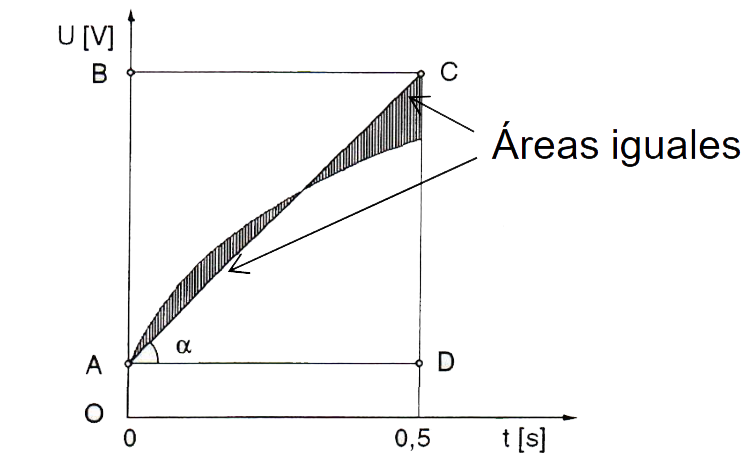
\includegraphics[width=1\linewidth]{res/tema7/tanAlpha}
				\end{minipage}
			\end{figure}
					
		\subsection{Clasificación de los sistemas de excitación.}
			\subsubsection{Excitación estática o directa, autoexcitada con anillos y escobillas.}
				\begin{figure}[H]
					\begin{minipage}{0.3\textwidth}
						Es un sistema autoexcitado de excitación independiente. Muy habitual en generadores de pequeña potencia. 
						
						\vspace{0.25cm}
						Se alimenta el inductor a través de anillos rozantes y escobillas. Es un sistema de respuesta rápida y es autónomo menos en el arranque. 
						
						\vspace{0.25cm}
						Tiene la desventaja de poder causar cortocircuitos en las partes metálicas puestas a tierra, como la armadura del motor.
					\end{minipage}
					\hspace{0.25cm}
					\begin{minipage}{0.6\textwidth}
						\begin{figure}[H]
							\centering
							\begin{circuitikz}
								\tikzstyle{every node}=[font=\normalsize]
								\draw  (13,14.25) circle (0.75cm);
								\draw  (13,13.5) circle (0.75cm);
								\draw  (14.5,11.75) circle (0.5cm);
								\draw  (15,11.75) circle (0.5cm);
								\draw (17.5,10.5) to[D] (16.5,10.5);
								\draw  (16.25,11) rectangle (17.75,10);
								\draw  (13,9.25) circle (1.5cm);
								\draw  (13,9.25) circle (1cm) node {\normalsize Rotor} ;
								\node [font=\normalsize] at (13,7.5) {Estátor};
								\draw [](13,10.75) to[short] (13,12.75);
								\draw[] (14,11.75) to[short] (13,11.75);
								\node at (13,11.75) [circ] {};
								\node [font=\normalsize] at (14.75,12.9) {Transformador};
								\node [font=\normalsize] at (14.75,12.5) {de excitación};
								\node [font=\normalsize, rotate around={90:(0,0)}] at (11.55,14) {Transformador};
								\node [font=\normalsize, rotate around={90:(0,0)}] at (12,14) {de potencia};
								\draw [](13,15) to[short] (13,16);
								\draw [](12.75,15.75) to[short] (13.25,15.75);
								\node [font=\normalsize, rotate around={-360:(0,0)}] at (14.75,15.75) {Red de transporte};
								\node [font=\normalsize, rotate around={-360:(0,0)}] at (15.25,10.6) {Puente de};
								\draw [](15.5,11.75) to[short] (17,11.75);
								\draw [](17,11.75) to[short] (17,11);
								\draw [](17,10) to[short] (17,9.25);
								\draw[] (17,9.25) to[short] (14,9.25);
								\node [font=\normalsize, rotate around={-360:(0,0)}] at (15.25,10.25) {tiristores};
								\node [font=\normalsize, rotate around={-360:(0,0)}] at (16.25,12) {c.a.};
								\node [font=\normalsize, rotate around={-360:(0,0)}] at (15.75,9.5) {c.c.};
								\draw [, rotate around={-360:(19.625, 10.5)}] (19,11) rectangle  node {\normalsize AVR} (20.25,10);
								\draw (19,10.5) to[short] (17.75,10.5);
							\end{circuitikz}
							
							\label{fig:my_label}
						\end{figure}
					\end{minipage}
				\end{figure}
				
		\subsubsection{Excitación estática o directa, con excitación independiente a través de servicios auxiliares.}
			\begin{figure}[H]
				\begin{minipage}{0.3\textwidth}
					Se alimenta de la red de servicios auxiliares o similar. 
					
					\vspace{0.25cm}
					Muy habitual en generadores de pequeña potencia. Utiliza escobillas y anillos rozantes. Respuesta rápida. 
					
					\vspace{0.25cm}
					Tiene la desventaja de tener una respuesta pobre ante cortocircuitos en la red.
				\end{minipage}
				\hspace{0.25cm}
				\begin{minipage}{0.6\textwidth}
					\begin{figure}[H]
						\centering
							\begin{circuitikz}
								\tikzstyle{every node}=[font=\LARGE]
								\draw  (13,14.25) circle (0.75cm);
								\draw  (13,13.5) circle (0.75cm);
								\draw  (17,13.25) circle (0.5cm);
								\draw  (17,12.75) circle (0.5cm);
								\draw (17.5,10.5) to[D] (16.5,10.5);
								\draw  (16.25,11) rectangle (17.75,10);
								\draw  (13,9.25) circle (1.5cm);
								\draw  (13,9.25) circle (1cm) node {\normalsize Rotor} ;
								\node [font=\normalsize] at (13,7.5) {Estátor};
								\draw [](13,10.75) to[short] (13,12.75);
								\node [font=\normalsize, rotate around={90:(0,0)}] at (15.9,13) {Servicios};
								\node [font=\normalsize, rotate around={90:(0,0)}] at (16.25,13) {auxiliares};
								\node [font=\normalsize, rotate around={90:(0,0)}] at (11.55,14) {Transformador};
								\node [font=\normalsize, rotate around={90:(0,0)}] at (12,14) {de potencia};
								\draw [](13,15) to[short] (13,16);
								\draw [](12.75,15.75) to[short] (13.25,15.75);
								\node [font=\normalsize, rotate around={-360:(0,0)}] at (14.75,15.75) {Red de transporte};
								\node [font=\normalsize, rotate around={-360:(0,0)}] at (15.25,10.6) {Puente de};
								\draw [](17,12.25) to[short] (17,11.75);
								\draw [](17,11.75) to[short] (17,11);
								\draw [](17,10) to[short] (17,9.25);
								\draw[] (17,9.25) to[short] (14,9.25);
								\node [font=\normalsize, rotate around={-360:(0,0)}] at (15.25,10.25) {tiristores};
								\node [font=\normalsize, rotate around={90:(0,0)}] at (16.75,11.75) {c.a.};
								\node [font=\normalsize, rotate around={-360:(0,0)}] at (15.75,9.5) {c.c.};
								\draw [, rotate around={-360:(19.625, 10.5)}] (19,11) rectangle  node {\normalsize AVR} (20.25,10);
								\draw[] (19,10.5) to[short] (17.75,10.5);
								\draw [](17,13.75) to[short] (17,14.5);
							\end{circuitikz}
						
						\label{fig:my_label}
					\end{figure}
				\end{minipage}
			\end{figure}
			
		\subsubsection{Excitación rotativa o indirecta, con excitatriz de c.c. sin excitatriz piloto.}
			\begin{figure}[H]
				\begin{minipage}{0.3\textwidth}
					Una máquina de c.c. alimenta el inductor a través de anillos rozantes y escobillas. Unida al eje del generador.
					
					\vspace{0.25cm}
					Para generadores hidráulicos de hasta $50\,MV\!A$. 
					
					\vspace{0.25cm}
					Alimentación independiente mediante red auxiliar.
				\end{minipage}
				\hspace{0.25cm}
				\begin{minipage}{0.6\textwidth}
					\begin{figure}[H]
						\centering
							\begin{circuitikz}
								\tikzstyle{every node}=[font=\normalsize]
								\draw  (13,14.25) circle (0.75cm);
								\draw  (13,13.5) circle (0.75cm);
								\draw  (18.5,14) circle (0.5cm);
								\draw  (18.5,13.5) circle (0.5cm);
								\draw (19,11.25) to[D] (18,11.25);
								\draw  (17.75,11.75) rectangle (19.25,10.75);
								\draw  (13,9.25) circle (1.5cm);
								\draw  (13,9.25) circle (1cm) node {\normalsize Generador} ;
								\draw [](13,10.75) to[short] (13,12.75);
								\node [font=\normalsize, rotate around={90:(0,0)}] at (17.4,13.75) {Servicios};
								\node [font=\normalsize, rotate around={90:(0,0)}] at (17.75,13.75) {auxiliares};
								\node [font=\normalsize, rotate around={90:(0,0)}] at (11.55,14) {Transformador};
								\node [font=\normalsize, rotate around={90:(0,0)}] at (12,14) {de potencia};
								\draw [](13,15) to[short] (13,16);
								\draw [](12.75,15.75) to[short] (13.25,15.75);
								\node [font=\normalsize, rotate around={-360:(0,0)}] at (14.75,15.75) {Red de transporte};
								\node [font=\normalsize, rotate around={-360:(0,0)}] at (16.75,11.3) {Puente de};
								\draw [](18.5,13) to[short] (18.5,12.5);
								\draw [](18.5,12.5) to[short] (18.5,11.75);
								\draw [](18.5,10.75) to[short] (18.5,10);
								\node [font=\normalsize, rotate around={-360:(0,0)}] at (16.75,11) {tiristores};
								\node [font=\normalsize, rotate around={90:(0,0)}] at (18.25,12.5) {c.a.};
								\draw [, rotate around={-360:(21.125, 11.25)}] (20.5,11.75) rectangle  node {\normalsize AVR} (21.75,10.75);
								\draw[] (20.5,11.25) to[short] (19.25,11.25);
								\draw [](18.5,14.5) to[short] (18.5,15.25);
								
								\draw  (16.5,9.25) circle (0.5cm);
								\draw  (16.5,9.25) circle (0.75cm) node {\normalsize Exc.} ;
								\draw [dashed] (14,9.25) -- (16,9.25);
								\draw [short] (13.75,9.875) -- (14.5,10.5);
								\draw [short] (13.75,8.625) -- (14.5,8);
								\draw [short] (14.5,10.5) -- (16.5,10.5);
								\draw [short] (16.5,10.5) -- (16.5,10);
								\draw [short] (16.5,8.5) -- (16.5,8);
								\draw [short] (16.5,8) -- (14.5,8);
								\node at (16.5,10) [circ] {};
								\node at (16.5,8.5) [circ] {};
								\draw [ fill={rgb,255:red,0; green,0; blue,0} , rotate around={-360:(17.625, 9.25)}] (17.5,10) rectangle (17.75,8.5);
								\draw [](18.5,10) to[short] (18.5,9.25);
								\draw[] (18.5,9.25) to[short] (17.75,9.25);
								\node [font=\normalsize, rotate around={90:(0,0)}] at (18.25,10) {c.c.};
								\node [font=\normalsize, rotate around={-360:(0,0)}] at (15.25,8.25) {c.c.};
							\end{circuitikz}
						
						\label{fig:my_label}
					\end{figure}
				\end{minipage}
			\end{figure}
					
		En el caso de un cortocircuito en la red, el inducido provoca un campo opuesto al campo principal, lo que provoca que la excitatriz tiene que suministrar una potencia más alta que en servicio nominal. Este exceso de tensión puede estar entre un 40 y un 80\% de la tensión nominal.
		
		
		
		
		
		
		
		
		
		
		\begin{figure}[H]
			\centering
				\begin{circuitikz}
					\tikzstyle{every node}=[font=\normalsize]
					\draw  (13,14.25) circle (0.75cm);
					\draw  (13,13.5) circle (0.75cm);
					\draw (16.75,11.25) to[D] (15.75,11.25);
					\draw  (15.5,11.75) rectangle (17,10.75);
					\draw  (13,9.25) circle (1.5cm);
					\draw  (13,9.25) circle (1cm) node {\normalsize Generador} ;
					\draw [](13,10.75) to[short] (13,12.75);
					\node [font=\normalsize, rotate around={90:(0,0)}] at (11.55,14) {Transformador};
					\node [font=\normalsize, rotate around={90:(0,0)}] at (12,14) {de potencia};
					\draw [](13,15) to[short] (13,16);
					\draw [](12.75,15.75) to[short] (13.25,15.75);
					\node [font=\normalsize, rotate around={-360:(0,0)}] at (14.75,15.75) {Red de transporte};
					\node [font=\normalsize, rotate around={-360:(0,0)}] at (16.25,10.5) {Puente de};
					\node [font=\normalsize, rotate around={-360:(0,0)}] at (16.25,10.175) {tiristores};
					
					\draw  (19.5,9.25) circle (0.5cm);
					\draw  (19.5,9.25) circle (0.75cm) node {\normalsize G} ;
					\draw [dashed] (14,9.25) -- (19,9.25);
					\draw [short] (13.75,9.875) -- (15,11.25);
					\draw [short] (15,11.25) -- (15.5,11.25);
					\draw [short] (17,11.25) -- (17.5,11.25);
					\draw [short] (17.5,11.25) -- (18.95,9.75);
					\draw [, rotate around={-360:(16.25, 12.75)}] (15.5,13.25) rectangle  node {\normalsize AVR} (17,12.25);
					\draw [](16.25,12.25) to[short] (16.25,11.75);
					\node [font=\normalsize, rotate around={-360:(0,0)}] at (19.5,10.75) {Imanes};
					\node [font=\normalsize, rotate around={-360:(0,0)}] at (19.5,10.5) {Permanentes};
				\end{circuitikz}
			
			\label{fig:my_label}
		\end{figure}
		
		
		
		\begin{figure}[H]
			\centering
				\begin{circuitikz}
					\tikzstyle{every node}=[font=\normalsize]
					\draw  (13,14.25) circle (0.75cm);
					\draw  (13,13.5) circle (0.75cm);
					\draw  (19.75,14) circle (0.5cm);
					\draw  (19.75,13.5) circle (0.5cm);
					\draw (20.25,11.25) to[D] (19.25,11.25);
					\draw  (19,11.75) rectangle (20.5,10.75);
					\draw  (13,9.25) circle (1.5cm);
					\draw  (13,9.25) circle (1cm) node {\normalsize Generador} ;
					\draw [](13,10.75) to[short] (13,12.75);
					\node [font=\normalsize, rotate around={90:(0,0)}] at (18.7,13.75) {Servicios};
					\node [font=\normalsize, rotate around={90:(0,0)}] at (19,13.75) {auxiliares};
					\node [font=\normalsize, rotate around={90:(0,0)}] at (11.65,14) {Transformador};
					\node [font=\normalsize, rotate around={90:(0,0)}] at (12,14) {de potencia};
					\draw [](13,15) to[short] (13,16);
					\draw [](12.75,15.75) to[short] (13.25,15.75);
					\node [font=\normalsize, rotate around={-360:(0,0)}] at (14.75,15.75) {Red de transporte};
					\node [font=\normalsize, rotate around={-360:(0,0)}] at (18,11.3) {Puente de};
					\draw [](19.75,13) to[short] (19.75,12.5);
					\draw [](19.75,12.5) to[short] (19.75,11.75);
					\draw [](19.75,10.75) to[short] (19.75,10);
					\node [font=\normalsize, rotate around={-360:(0,0)}] at (18,11) {tiristores};
					\node [font=\normalsize, rotate around={90:(0,0)}] at (19.5,12.5) {c.a.};
					\draw [, rotate around={-360:(22.375, 11.25)}] (21.75,11.75) rectangle  node {\normalsize AVR} (23,10.75);
					\draw[] (21.75,11.25) to[short] (20.5,11.25);
					\draw [](19.75,14.5) to[short] (19.75,15.25);
					
					\draw  (18.25,9.25) circle (0.5cm);
					\draw  (18.25,9.25) circle (0.75cm) node {\normalsize Exc.} ;
					\draw [short] (14,9.25) -- (15.25,9.25);
					\draw [](19.75,10) to[short] (19.75,9.25);
					\draw[] (19.75,9.25) to[short] (19,9.25);
					\node [font=\normalsize, rotate around={90:(0,0)}] at (19.5,10) {c.c.};
					\draw  (15.25,9.75) rectangle (16.75,8.75);
					\draw (16.5,9.25) to[D] (15.5,9.25);
					\draw [](16.75,9.25) to[short] (17.75,9.25);
					\node [font=\normalsize, rotate around={-360:(0,0)}] at (16,10.5) {Caja de};
					\node [font=\normalsize, rotate around={-360:(0,0)}] at (16,10.15) {diodos giratorios};
					\node [font=\normalsize, rotate around={-360:(0,0)}] at (17.2,9.5) {c.a.};
					\node [font=\normalsize, rotate around={-360:(0,0)}] at (14.85,9.5) {c.c.};
				\end{circuitikz}
			
			\label{fig:my_label}
		\end{figure}
		
		
		
		
		
		\begin{figure}[H]
			\centering
				\begin{circuitikz}
					\tikzstyle{every node}=[font=\normalsize]
					\draw  (13,14.25) circle (0.75cm);
					\draw  (13,13.5) circle (0.75cm);
					\draw  (15.75,12) circle (0.5cm);
					\draw  (16.25,12) circle (0.5cm);
					\draw (20.25,10.75) to[D] (19.25,10.75);
					\draw  (19,11.25) rectangle (20.5,10.25);
					\draw  (13,9.25) circle (1.5cm);
					\draw  (13,9.25) circle (1cm) node {\normalsize Generador} ;
					\draw [](13,10.75) to[short] (13,12.75);
					\node [font=\normalsize, rotate around={-360:(0,0)}] at (16,13.1) {Transformador};
					\node [font=\normalsize, rotate around={-360:(0,0)}] at (16,12.75) {de excitación};
					\node [font=\normalsize, rotate around={90:(0,0)}] at (11.65,14) {Transformador};
					\node [font=\normalsize, rotate around={90:(0,0)}] at (12,14) {de potencia};
					\draw [](13,15) to[short] (13,16);
					\draw [](12.75,15.75) to[short] (13.25,15.75);
					\node [font=\normalsize, rotate around={-360:(0,0)}] at (14.75,15.75) {Red de transporte};
					\node [font=\normalsize, rotate around={-360:(0,0)}] at (18,11) {Puente de};
					\draw [](19.75,12) to[short] (19.75,11.25);
					\draw [](19.75,10.25) to[short] (19.75,10);
					\node [font=\normalsize, rotate around={-360:(0,0)}] at (18,10.6) {tiristores};
					\node [font=\normalsize, rotate around={-360:(0,0)}] at (18.25,12.25) {c.a.};
					\draw [, rotate around={-360:(22.375, 10.75)}] (21.75,11.25) rectangle  node {\normalsize AVR} (23,10.25);
					\draw[] (21.75,10.75) to[short] (20.5,10.75);
					
					\draw  (18.25,9.25) circle (0.5cm);
					\draw  (18.25,9.25) circle (0.75cm) node {\normalsize Exc.} ;
					\draw [short] (14,9.25) -- (15.25,9.25);
					\draw [](19.75,10) to[short] (19.75,9.25);
					\draw[] (19.75,9.25) to[short] (19,9.25);
					\node [font=\normalsize, rotate around={90:(0,0)}] at (19.5,9.75) {c.c.};
					\draw  (15.25,9.75) rectangle (16.75,8.75);
					\draw (16.5,9.25) to[D] (15.5,9.25);
					\draw [](16.75,9.25) to[short] (17.75,9.25);
					\node [font=\normalsize, rotate around={-360:(0,0)}] at (16,10.5) {Caja de};
					\node [font=\normalsize, rotate around={-360:(0,0)}] at (16,10.15) {diodos giratorios};
					\node [font=\normalsize, rotate around={-360:(0,0)}] at (17.2,9.5) {c.a.};
					\node [font=\normalsize, rotate around={-360:(0,0)}] at (14.85,9.5) {c.c.};
					\draw [](16.75,12) to[short] (19.75,12);
					\draw[] (15.25,12) to[short] (13,12);
					\node at (13,12) [circ] {};
				\end{circuitikz}
			
			\label{fig:my_label}
		\end{figure}
		
		
		
		\begin{figure}[H]
			\centering
				\begin{circuitikz}
					\tikzstyle{every node}=[font=\normalsize]
					\draw  (10,12.75) circle (1.5cm);
					\draw  (10,12.75) circle (1cm);
					\draw (10,13.5) to[L ] (10,12);
					\draw [dashed] (10,12.75) -- (18.5,12.75);
					\draw [ fill={rgb,255:red,0; green,0; blue,0} , rotate around={-360:(12.625, 12.75)}] (12.5,13.25) rectangle (12.75,12.25);
					\draw [ fill={rgb,255:red,0; green,0; blue,0} , rotate around={-360:(13.125, 12.75)}] (13,13.25) rectangle (13.25,12.25);
					\draw  (15,12.75) circle (0.5cm);
					\node at (15,13.25) [circ] {};
					\node at (15,12.25) [circ] {};
					\draw [](10,12) to[short] (11.75,12);
					\draw [](11.75,12) to[short] (11.75,12.25);
					\draw [](11.75,12.25) to[short] (11.75,12.5);
					\draw [](11.75,12.5) to[short] (13,12.5);
					\draw [](10,13.5) to[short] (11.75,13.5);
					\draw [](11.75,13.5) to[short] (11.75,13);
					\draw [](11.75,13) to[short] (12.5,13);
					\draw [](12.625,13.25) to[short] (12.625,13.75);
					\draw [](12.625,13.75) to[short] (15,13.75);
					\draw [](15,13.75) to[short] (15,13.25);
					\draw [](15,12.25) to[short] (15,11.75);
					\draw[] (15,11.75) to[short] (13.125,11.75);
					\draw [](13.125,11.75) to[short] (13.125,12.25);
					\draw (16,13.5) to[L ] (16,12);
					\draw  (18.5,12.75) circle (0.5cm);
					\draw [](18.5,13.25) to[short] (18.5,13.75);
					\draw [](18.5,12.25) to[short] (18.5,11.75);
					\draw (16,13.75) to[R] (17.5,13.75);
					\draw [->, >=Stealth] (16.75,14.5) -- (16.75,14);
					\draw [short] (16.75,14.5) -- (18.5,14.5);
					\draw [short] (18.5,14.5) -- (18.5,13.75);
					\draw [short] (16,13.75) -- (16,13.5);
					\draw [short] (18.5,11.75) -- (16,11.75);
					\draw [short] (16,11.75) -- (16,12);
					\draw (19.5,13.5) to[L ] (19.5,12);
					\draw [](19.5,13.5) to[short] (19.5,14.5);
					\draw[] (19.5,14.5) to[short] (18.5,14.5);
					\draw [](18.5,11.75) to[short] (19.5,11.75);
					\draw [](19.5,11.75) to[short] (19.5,12);
					\node at (18.5,14.5) [circ] {};
					\node at (18.5,11.75) [circ] {};
					\node [font=\normalsize, rotate around={-360:(0,0)}] at (18.25,13.5) {+};
					\node [font=\normalsize, rotate around={-360:(0,0)}] at (14.75,13.5) {+};
					\node [font=\normalsize, rotate around={-360:(0,0)}] at (15.5,11.4) {Excitatriz};
					\node [font=\normalsize, rotate around={-360:(0,0)}] at (15.5,11.1) {principal};
					\node [font=\normalsize, rotate around={-360:(0,0)}] at (19,11.4) {Excitatriz};
					\node [font=\normalsize, rotate around={-360:(0,0)}] at (19,11.1) {piloto};
					\draw (7,12.75) to[tmultiwire= \normalsize Red] (8.5,12.75);
				\end{circuitikz}
			
			\label{fig:my_label}
		\end{figure}
					
					
					
		\begin{figure}[H]
			\centering
				\begin{circuitikz}
					\tikzstyle{every node}=[font=\normalsize]
					\draw  (10,12.75) circle (1.5cm);
					\draw  (10,12.75) circle (1cm);
					\draw (10,13.5) to[L ] (10,12);
					\draw [dashed] (10,12.75) -- (18,12.75);
					\draw [ fill={rgb,255:red,0; green,0; blue,0} , rotate around={-360:(12.625, 12.75)}] (12.5,13.25) rectangle (12.75,12.25);
					\draw [ fill={rgb,255:red,0; green,0; blue,0} , rotate around={-360:(13.125, 12.75)}] (13,13.25) rectangle (13.25,12.25);
					\draw [](10,12) to[short] (11.75,12);
					\draw [](11.75,12) to[short] (11.75,12.25);
					\draw [](11.75,12.25) to[short] (11.75,12.5);
					\draw [](11.75,12.5) to[short] (13,12.5);
					\draw [](10,13.5) to[short] (11.75,13.5);
					\draw [](11.75,13.5) to[short] (11.75,13);
					\draw [](11.75,13) to[short] (12.5,13);
					\draw [](13.125,13.25) to[short] (13.125,14.5);
					\draw [](7,12.75) to[tmultiwire= \normalsize Red] (8.5,12.75);
					\draw (15,14.75) to[D] (14,14.75);
					\draw [, rotate around={-360:(14.5, 14.75)}] (13.75,15.25) rectangle (15.25,14.25);
					\draw [short] (13.125,14.5) -- (13.75,14.5);
					\draw [short] (13.75,15) -- (12.625,15);
					\draw [short] (12.625,15) -- (12.625,13.25);
					\draw [short] (15.25,14.75) -- (16.25,14.75);
					\draw  (16.25,12.75) circle (1cm);
					\draw  (16.25,12.75) circle (1.25cm);
					\draw (16.25,13.5) to[L ] (16.25,12);
					\draw [](16.25,14) to[tmultiwire] (16.25,14.75);
					\draw [](16.25,13.5) to[short] (18,13.5);
					\draw [](16.25,12) to[short] (18,12);
					\draw (18.5,12.25) to[D] (18.5,13.25);
					\draw [, rotate around={-360:(18.5, 12.75)}] (18,13.75) rectangle (19,11.75);
					\draw [dashed] (19,12.75) -- (20.5,12.75);
					\draw  (21,12.75) circle (0.75cm) node {\normalsize Exc.} ;
					\draw  (21,12.75) circle (0.5cm);
					\draw[] (21,14.25) to[tmultiwire] (18.5,14.25);
					\draw [](21,14.25) to[short] (21,13.5);
					\draw [](18.5,14.25) to[short] (18.5,13.75);
					\node [font=\normalsize, rotate around={-360:(0,0)}] at (16.75,11.25) {Excitatriz principal};
					\node [font=\normalsize, rotate around={-360:(0,0)}] at (16.75,10.8) {de corriente alterna};
					\node [font=\normalsize, rotate around={-360:(0,0)}] at (21,11.25) {Excitatriz piloto};
					\node [font=\normalsize, rotate around={-360:(0,0)}] at (21,10.8) {de imanes permanentes};
					\node [font=\normalsize, rotate around={-360:(0,0)}] at (10,11) {Alternador};
				\end{circuitikz}
			
			\label{fig:my_label}
		\end{figure}
		
		
		
		\begin{figure}[H]
			\centering
				\begin{circuitikz}
					\tikzstyle{every node}=[font=\normalsize]
					\draw (22.75,10.5) to[D] (21.75,10.5);
					\draw  (21.5,11) rectangle (23,10);
					\draw  (13,9.75) circle (1.5cm);
					\draw  (13,9.75) circle (1cm) node {\normalsize Generador} ;
					\node [font=\normalsize, rotate around={-360:(0,0)}] at (24,11.25) {Puente de tiristores};
					
					\draw  (18.25,9.75) circle (0.5cm);
					\draw  (18.25,9.75) circle (0.75cm) node {\normalsize Exc.} ;
					\draw [short] (14,9.75) -- (15.25,9.75);
					\draw[] (21.5,10.5) to[short] (21,10.5);
					\node [font=\normalsize, rotate around={-360:(0,0)}] at (20.75,10.75) {c.c.};
					\draw  (15.25,10.25) rectangle (16.75,9.25);
					\draw (16.5,9.75) to[D] (15.5,9.75);
					\draw [](16.75,9.75) to[short] (17.75,9.75);
					\node [font=\normalsize, rotate around={-360:(0,0)}] at (16,8.75) {Caja de};
					\node [font=\normalsize, rotate around={-360:(0,0)}] at (16,8.375) {diodos giratorios};
					\node [font=\normalsize, rotate around={-360:(0,0)}] at (17.2,9.5) {c.a.};
					\node [font=\normalsize, rotate around={-360:(0,0)}] at (14.85,9.5) {c.c.};
					\draw  (10.25,9.75) circle (0.5cm) node {\normalsize M} ;
					\draw [dashed] (10.75,9.75) -- (12,9.75);
					\draw  (21.5,12.25) rectangle  node {\normalsize AVR} (23,11.5);
					\draw [short] (22.25,11.5) -- (22.25,11);
					\draw (19,9.75) to[R] (21,9.75);
					\draw [->, >=Stealth] (20,10.5) -- (20,10);
					\draw [short] (20,10.5) -- (21,10.5);
					\draw [](13,11.25) to[tmultiwire= \normalsize Red] (13,12.25);
					\draw  (24.5,9.75) circle (0.5cm) node {\normalsize G} ;
					\draw [dashed] (24,9.75) -- (21.25,9.75);
					\draw [](23,10.5) to[tmultiwire] (24.5,10.5);
					\draw [](24.5,10.5) to[short] (24.5,10.25);
					\node [font=\normalsize] at (10.25,11) {Motor};
					\node [font=\normalsize] at (10.25,10.625) {primario};
					\node [font=\normalsize] at (24.5,9) {Excitatriz piloto};
					\node [font=\normalsize] at (24.5,8.625) {de imanes permanentes};
					\node [font=\normalsize] at (18.25,11.5) {Excitatriz principal};
					\node [font=\normalsize] at (18.25,11.125) {de corriente};
					\node [font=\normalsize] at (18.25,10.75) {alterna};
				\end{circuitikz}
			
			\label{fig:my_label}
		\end{figure}
				
	
	\begin{figure}[H]
		\centering
		\begin{circuitikz}
			\tikzstyle{every node}=[font=\normalsize]
			\draw [short] (7.25,10.25) -- (7.25,8.75);
			\draw [short] (6.25,9.25) -- (7.25,8.75);
			\draw [short] (6.25,9.75) -- (7.25,10.25);
			\node [font=\normalsize] at (3.5,10.75) {};
			\node [font=\normalsize] at (6.75,9.5) {TV};
			\draw [short] (7.25,9.75) -- (9,9.75);
			\draw [short] (7.25,9.25) -- (9,9.25);
			\draw [short] (9.75,10) -- (10,10);
			\draw [short] (10,10) -- (10,9.75);
			\draw [short] (9.75,9) -- (10,9);
			\draw [short] (10,9) -- (10,9.25);
			\draw [short] (10,9.25) -- (11.8,9.25);
			\draw [short] (10,9.75) .. controls (12.5,9.75) and (10.25,9.75) .. (11.8,9.75);
			\draw  (12.5,9.5) circle (0.75cm) node {\normalsize G} ;
			\draw [line width=0.2pt, short] (12.25,9.25) .. controls (12.5,9.5) and (12.5,9) .. (12.75,9.25);
			\draw [short] (13.25,9.5) -- (15.5,9.5);
			\draw [short] (14.75,9.5) -- (14.75,7);
			\draw  (11.5,7.5) rectangle (13.5,6.5);
			\node [font=\normalsize] at (12.5,7.25) {Regulador};
			\node [font=\normalsize] at (12.5,6.75) {AVR};
			\draw (11.75,8.25) to[L ] (13.25,8.25);
			\draw [short] (11.75,8.25) -- (11.75,7.5);
			\draw [short] (13.25,8.25) -- (13.25,7.5);
			\draw [line width=0.2pt, short] (13.5,9.25) -- (13.75,9.75);
			\draw [line width=0.2pt, short] (13.75,9.25) -- (14,9.75);
			\draw [line width=0.2pt, short] (14,9.25) -- (14.25,9.75);
			\draw [line width=0.2pt, short] (14.25,9.25) -- (14.5,9.75);
			\draw [short] (9.75,10) -- (9.75,11.25);
			\draw [short] (9.75,10) -- (9.5,10);
			\draw [short] (9.5,10) -- (9.5,9.75);
			\draw [short] (9.5,9.25) -- (9.5,9);
			\draw [short] (9.5,9) -- (9.75,9);
			\draw [short] (9,9.75) -- (9.5,9.75);
			\draw [short] (9,9.25) -- (9.5,9.25);
			\draw [short] (6.25,9.75) -- (6.25,9.25);
			\draw  (8.75,12.25) rectangle (10.75,11.25);
			\node [font=\normalsize] at (9.75,12) {Regulador};
			\node [font=\normalsize] at (9.75,11.5) {velocidad};
			\draw [->, >=Stealth] (8,10) .. controls (8.25,9.5) and (8.25,9.5) .. (8,9) ;
			\draw [->, >=Stealth] (8.75,10) .. controls (9,9.5) and (9,9.5) .. (8.75,9) ;
			\draw [->, >=Stealth] (11.25,9) .. controls (11,9.5) and (11,9.5) .. (11.25,10) ;
			\node [font=\normalsize] at (8,8.75) {n};
			\node [font=\normalsize] at (10,10.75) {n};
			\node [font=\normalsize] at (11.25,10.25) {$T_{elec}$};
			\node [font=\normalsize] at (8.75,8.75) {$T_{mec}$};
			\draw [->, >=Stealth] (9.75,10) -- (9.75,11.25);
			\draw [->, >=Stealth] (12,11.75) -- (10.75,11.75);
			\draw [->, >=Stealth] (12.5,5.75) -- (12.5,6.5);
			\draw [->, >=Stealth] (11.5,7.75) -- (11.5,8.25);
			\draw [->, >=Stealth] (14.75,7) -- (13.5,7);
			\node [font=\normalsize] at (14.75,8.25) {};
			\node [font=\normalsize] at (12.5,5.5) {$V_{ref}$};
			\node [font=\normalsize] at (11.25,8) {$I_{ex}$};
			\node [font=\normalsize] at (15,8) {V};
			\node [font=\normalsize] at (12.5,11.75) {$P_{ref}$};
			\draw  (8,11.75) circle (0.5cm);
			\draw [short] (8.75,11.75) -- (8.5,11.75);
			\node [font=\normalsize] at (8,11.75) {$M$};
			\draw [short] (7.5,11.75) -- (5.75,11.75);
			\draw [->, >=Stealth] (5.75,11.75) -- (5.75,11.25);
			\draw [short] (5.75,11.25) -- (6.25,11.5);
			\draw [short] (5.75,11.25) -- (6.25,11);
			\draw [short] (6.25,11) -- (6.25,11.5);
			\draw [short] (5.75,11.25) -- (5.25,11.5);
			\draw [short] (5.25,11.5) -- (5.25,11);
			\draw [short] (5.25,11) -- (5.75,11.25);
			\draw [short] (6.75,10) -- (6.75,11.25);
			\draw [short] (6.25,11.25) -- (6.75,11.25);
			\draw [short] (5.25,11.25) -- (4.75,11.25);
			\node [font=\normalsize] at (8,12.5) {$Servomotor$};
			\node [font=\normalsize] at (4,11.5) {$Entrada$};
			\node [font=\normalsize] at (4,11) {$vapor$};
			\draw [ color={rgb,255:red,2; green,141; blue,37} , dashed] (10.5,10.75) rectangle  (16,5);
			\draw [ color={rgb,255:red,234; green,72; blue,72}, dashed] (13,10.75) -- (13,13.5);
			\draw [ color={rgb,255:red,234; green,72; blue,72}, dashed] (13,13.5) -- (3.25,13.5);
			\draw [ color={rgb,255:red,234; green,72; blue,72}, dashed] (3.25,13.5) -- (3.25,7.75);
			\draw [ color={rgb,255:red,234; green,72; blue,72}, dashed] (3.25,7.75) -- (10.5,7.75);
			\node [font=\normalsize, color={rgb,255:red,234; green,72; blue,72}] at (4.25,13) {Control P-f};
			\node [font=\normalsize, color={rgb,255:red,62; green,167; blue,89}] at (14.75,5.5) {Control Q-V};
		\end{circuitikz}
		\label{fig:my_label}
	\end{figure}


		\chapter{Esquema TT. Protección diferencial}
\section{Análisis del esquema TT}
En este esquema están conectados a tierra tanto el centro de la estrella del transformador como las masas. Se produce un defecto fase-tierra con tierra de retorno.
\begin{figure}[H]
	\centering
	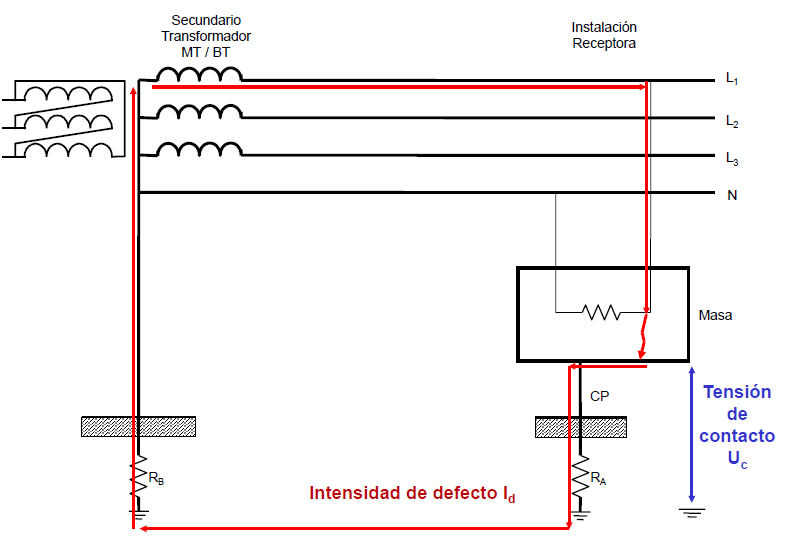
\includegraphics[width=0.5\linewidth]{Images/26}
	\label{fig:26}
\end{figure}

Su circuito equivalente es:
\begin{figure}[H]
	\centering
	\begin{adjustbox}{width=1\textwidth}
	
		\begin{circuitikz}
			\tikzstyle{every node}=[font=\normalsize]
			\draw (5.25,14.25) to[sinusoidal voltage source, sources/symbol/rotate=auto,l={ \normalsize $cU_{\text{fase-neutro}}$}] (5.25,11.25);
			\draw (6,15.5) to[european resistor,l={ \normalsize $\dfrac{2}{3} Z_{\text{media tension}}$}] (11,15.5);
			\draw (5.25,14.25) to[short] (5.25,15.5);
			\draw (5.25,15.5) to[short] (6.25,15.5);
			\draw (11,15.5) to[european resistor,l={ \normalsize $Z_{\text{trafo}}$}] (13.5,15.5);
			\draw (13.5,15.5) to[european resistor,l={ \normalsize $R_{\text{línea}}$}] (15.5,15.5);
			\draw (15.5,15.5) to[european resistor,l={ \normalsize $R_{\text{defecto}}$}] (15.5,12.75);
			\draw (15.5,12.75) to[european resistor,l={ \normalsize $R_{\text{cable protección}}$}] (15.5,10.75);
			\draw (15.5,10.75) to[european resistor,l={ \normalsize $R_{\text{puesta a tierra masas utilización}}$}] (15.5,8.5);
			\draw (5.25,11.25) to[european resistor,l={ \normalsize $R_{\text{puesta a tierra neutro}}$}] (5.25,8.5);
			\draw (5.25,8.5) to (5.25,8.25) node[ground]{};
			\draw (15.5,8.5) to (15.5,8.25) node[ground]{};
			\draw [ color={rgb,255:red,200; green,0; blue,255}, <->, >=Stealth] (14.25,13) -- (14.25,7.75)node[pos=0.5, fill=white]{$U_{contacto}$};
			\draw [ color={rgb,255:red,200; green,0; blue,255}, ->, >=Stealth] (8.5,14.75) -- (12.5,14.75)node[pos=0.5, fill=white]{$I_{defecto}$};
			\node [font=\normalsize, color={rgb,255:red,200; green,0; blue,255}] at (8.5,16.25) {$Z_{MT}$};
			\node [font=\normalsize, color={rgb,255:red,200; green,0; blue,255}] at (12.25,16.25) {$Z_T$};
			\node [font=\normalsize, color={rgb,255:red,200; green,0; blue,255}] at (14.5,16.25) {$R_F$};
			\node [font=\normalsize, color={rgb,255:red,200; green,0; blue,255}] at (16.5,14.5) {$R_d$};
			\node [font=\normalsize, color={rgb,255:red,200; green,0; blue,255}] at (16.5,12.25) {$R_{CP}$};
			\node [font=\normalsize, color={rgb,255:red,200; green,0; blue,255}] at (16.5,10) {$R_A$};
			\node [font=\normalsize, color={rgb,255:red,200; green,0; blue,255}] at (6.5,10.25) {$R_B$};
			\node [font=\normalsize, color={rgb,255:red,200; green,0; blue,255}] at (6.5,13.25) {$cU_0$};
		\end{circuitikz}
	\end{adjustbox}
	\label{fig:my_label}
\end{figure}

En estas condiciones:
\begin{equation}
	Z_{bucle}=\dfrac{2}{3}Z_{MT}+Z_T+Z_F+R_d+R_{CP}+R_A+R_B
\end{equation}
\begin{equation}
	I_d=\dfrac{c U_0}{Z_{bucle}}
\end{equation}
\begin{equation}
	U_c=\left(R_{CP}+R_A\right)I_d
\end{equation}
\subsection{Circuito equivalente simplificado en caso de fallo}
Normalmente las resistencias de puesta a tierra son mayores que el resto de impedancias:
\begin{equation}
	R_B+R'_A \ggg \dfrac{2}{3}Z_{MT}+Z_T+Z_F+R_d
\end{equation}

El caso más desfavorable desde el punto de vista de la protección:
\begin{equation}
	R_d=0
\end{equation}

La resistencia desde la masa de utilización a tierra:
\begin{equation}
	R_A'=R_A+R_{CP}
\end{equation}
\begin{center}
	\begin{figure}[H]
		\centering
	\begin{adjustbox}{width=0.5\textwidth}
		
		\begin{circuitikz}
			\tikzstyle{every node}=[font=\normalsize]
			\draw (5.25,14.25) to[sinusoidal voltage source, sources/symbol/rotate=auto,l={ \normalsize $cU_0$}] (5.25,11.25);
			\draw (5.25,14.25) to[short] (5.25,15.5);
			\draw (5.25,15.5) to[short] (6.25,15.5);
			\draw (15.5,10.75) to[european resistor] (15.5,8.5);
			\draw (5.25,11.25) to[european resistor] (5.25,8.5);
			\draw (5.25,8.5) to (5.25,8.25) node[ground]{};
			\draw (15.5,8.5) to (15.5,8.25) node[ground]{};
			\draw [ color={rgb,255:red,200; green,0; blue,255}, <->, >=Stealth] (14.25,10.75) -- (14.25,7.75)node[pos=0.5, fill=white]{$U_{contacto}$};
			\draw [ color={rgb,255:red,200; green,0; blue,255}, ->, >=Stealth] (8.5,14.75) -- (12.5,14.75)node[pos=0.5, fill=white]{$I_{defecto}$};
			\node [font=\normalsize, color={rgb,255:red,200; green,0; blue,255}] at (16.25,9.5) {$R_A$};
			\node [font=\normalsize, color={rgb,255:red,200; green,0; blue,255}] at (6,10) {$R_B$};
			\draw (6.25,15.5) to[short] (15.5,15.5);
			\draw (15.5,10.75) to[short] (15.5,15.5);
		\end{circuitikz}
	\end{adjustbox}
	\label{fig:my_label}
\end{figure}
\end{center}

En estas condiciones:
\begin{equation}
	R_S=R_{CP}+R_A+R_B
\end{equation}
\begin{equation}
	I_d=\dfrac{c U_0}{R_S}
\end{equation}
\begin{equation}
	U_c=\left(R_{CP}+R_A\right)I_d
\end{equation}

\textbf{Se debe disparar en caso de defecto mediante un interruptor diferencial.}
\section{Condiciones de protección}
\section{Interruptor diferencial}
\section{Selección de interruptores diferenciales}
\section{Selectividad entre interruptores diferenciales}
\section{Protección contra incendios}
\section{Ejemplo de cálculo de esquema TT}
\subsection{Datos de partida}
\subsection{Esquema eléctrico multifilar}
\subsection{Bucle de defecto}
\subsection{Circuito equivalente}
\subsection{Circuito equivalente simplificado}
\subsection{Cálculo de impedancia serie, corriente de defecto y tensión de contacto}
\subsection{Sensibilidad del interruptor diferencial}
\subsection{Comprobación del REBT esquema TT}
\subsection{Curvas de seguridad de tensión}
\subsection{Comprobar que se cumplen las curvas de seguridad de tiempo-intensidad}

		\chapter{Ejercicios resueltos.}
\section{Fundamentos y propiedades de los fluidos.}
\begin{enumerate}
	\item Obtener el ángulo de mojabilidad $\theta_c$.
	\begin{figure}[H]
		\begin{minipage}{0.7\textwidth}
		\centering
		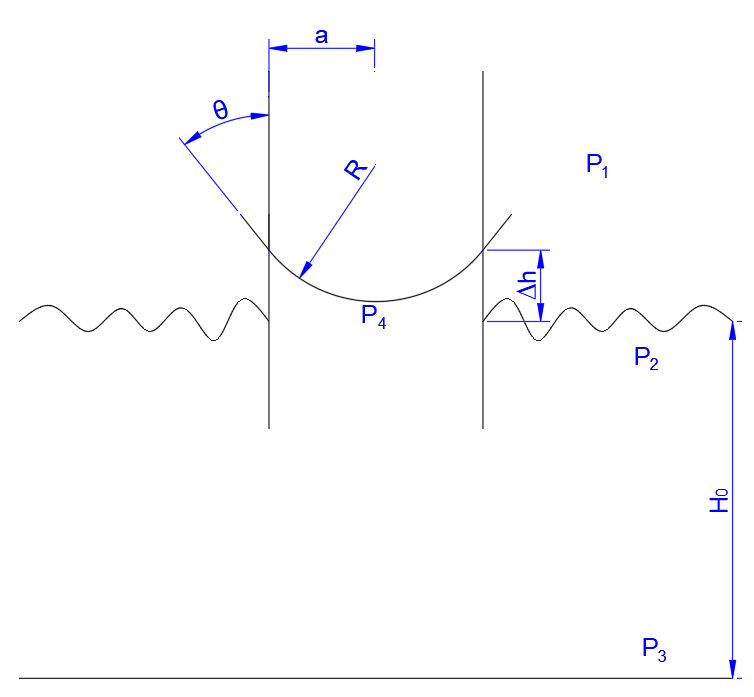
\includegraphics[width=0.65\linewidth]{imagenesEjercicios/mojabilidad}
		\caption{Esquema del problema.}
		\label{fig:mojabilidad}
	\end{minipage}%
	\begin{minipage}{0.3\textwidth}
	\[\textcolor{blue}{P_2=P_1=P_a}\]
	\[\textcolor{blue}{P_2=\rho g H_0=P_3}\]
	\[\textcolor{blue}{P_3=P_4+\rho g (H_0+\Delta h)}\]
	\[\textcolor{blue}{P_1-P_4=\dfrac{2\sigma}{R}}\]
	\[\textcolor{blue}{\dfrac{2\sigma}{R}=\rho g \Delta h}\]
	\[\textcolor{blue}{Rcos(\theta_c)=a}\]
	\[\textcolor{blue}{\theta_c=arccos\left(\dfrac{a\rho g \Delta h}{2\sigma}\right)}\]
	\end{minipage}
	\end{figure}
	
	\item Se ha instalado un nuevo sistema de presión para el abastecimiento
	de agua de un municipio. El agua procedente de un manantial es impulsado por una bomba
	y se almacena en un depósito sobrepresor. Para controlar la presión del agua a la entrada
	y salida de la bomba se han montado un vacuómetro y un manómetro en los puntos de
	interés. Cuando el vacuómetro marca 0.75 bares y el manómetro marca 4.2 bares. ¿Cuál
	será el valor de la presión absoluta? ¿Existe riesgo de cavitación en algún punto de la
	conducción? Datos: $p_{atm}$ = 816,91 hPa; $p_v$=159856 Pa.
	\begin{figure}[H]
		\begin{minipage}{0.7\textwidth}
		%\centering
		%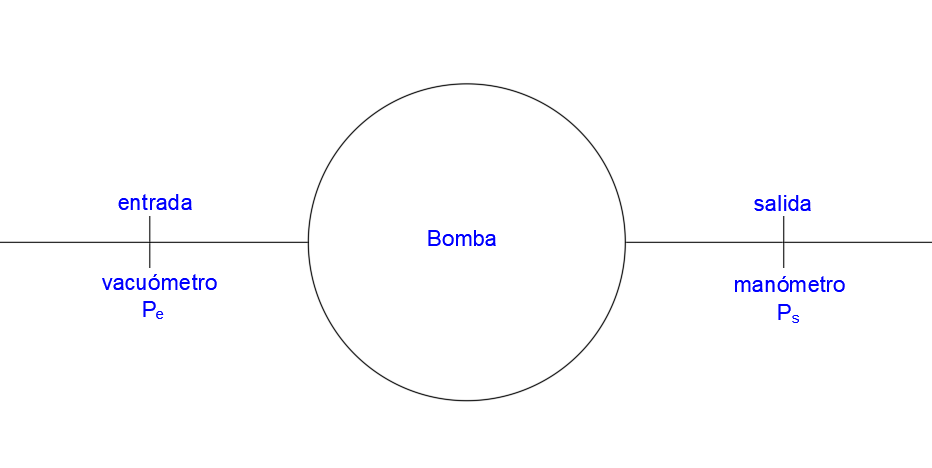
\includegraphics[width=0.7\linewidth]{imagenesEjercicios/bombaAisa}
		%\caption{Esquema bomba de agua.}
		%\label{fig:bombaaisa}
		\begin{figure}[H]
			\centering
				\begin{circuitikz}[scale = 0.9]
					\tikzstyle{every node}=[font=\normalsize]
					\draw  (4.75,20) circle (0.75cm) node {\normalsize Bomba} ;
					\draw [short] (5.5,20) -- (7,20);
					\draw [short] (6.25,20.25) -- (6.25,19.75)node[pos=0,above]{Salida};
					\node [font=\normalsize] at (7.25,19.5) {Manómetro $(P_S)$};
					\draw[] (4,20) to[short] (2.5,20);
					\draw [short] (3.25,20.25) -- (3.25,19.75)node[pos=0,above]{Entrada};
					\node [font=\normalsize] at (2.5,19.5) {Vacuómetro $(P_0)$};
				\end{circuitikz}
			
			\label{fig:my_label}
		\end{figure}
		\end{minipage}%
	\begin{minipage}{0.3\textwidth}
	\[\textcolor{blue}{P_v=P_{atm}-P_e}\]
	\[\textcolor{blue}{P_m=P_s-P_{atm}}\]
\[ \textcolor{blue}{P_e=81691-75000=6691 Pa}\]
\[\textcolor{blue}{P_s=81691+420000=501691 Pa}\]
\textcolor{blue}{Existe cavitación a la entrada.}
	
	\end{minipage}
\end{figure}

	\newpage
	\item La presión en un punto de un fluido ($\rho = 1234 \dfrac{kg}{m^3}$) alcanza el valor de 3 bares. Expresar
	el valor de la presión en milímetros de mercurio (cm Hg) y en columna de metros de agua
	(m.c.a.). Datos: $\rho_{Hg,rel} = 13,6$
	\[\textcolor{blue}{\rho = 1234 \dfrac{kg}{m^3}}\]
	\[\textcolor{blue}{P=3\cdot10^5 Pa}\]
	\[\textcolor{blue}{1mmHg=\rho_{Hg}g h=13.6\cdot10^3\dfrac{kg}{m^3} \cdot9.8 \dfrac{m}{s^2}\cdot10^{-3}m=133.416Pa} \]
	\[\textcolor{blue}{1mca=\rho_{H_2O}g h=10^3\dfrac{kg}{m^3}\cdot9.8 \dfrac{m}{s^2}\cdot1m=9810Pa}\]
	\item Sobre una superficie de 4000 $cm^2$, orientada en el espacio por su vector normal $\vec{n}=\vec{k}$, está
	actuando una fuerza$\vec{F}=2\vec{i}+3\vec{j}-3\vec{k}$ (N). Calcular la componente normal de la fuerza y
	la presión que está soportando la superficie
		\[\textcolor{blue}{S=4000 cm^2=0.4 m^2}\]
	\[\textcolor{blue}{\vec{n}=\vec{k}}\]
	\[\textcolor{blue}{\vec{F}=2\vec{i}+3\vec{j}-3\vec{k} \rightarrow F_n=3N}\]
	\[\textcolor{blue}{P=\dfrac{F_n}{S}=\dfrac{3 N}{0.4 m^2}=7.5Pa}\]
	
	\item Sabiendo que un fluido tiene una densidad de 0.627 $\dfrac{kg}{l}$ y que su coeficiente de viscosidad
	absoluta es 1.2 cP, calcular su viscosidad cinemática. ¿Cuál es su densidad relativa si
	consideramos el agua como fluido de referencia?. Datos $\rho_{agua} = 999,8\dfrac{kg}{m^3}$
\[\textcolor{blue}{\nu = \dfrac{\mu}{\rho}=\dfrac{1.2 cP \cdot \dfrac{10^{-3} Pa \cdot s}{1 cP}}{0.627 \dfrac{kg}{l}\cdot\dfrac{10^3 l}{m^3}}=1.91\cdot10^{-6}\dfrac{m^2}{s}}\]
\[\textcolor{blue}{\rho_{rel}=\dfrac{\rho}{\rho_{H_2O}}=\dfrac{0.627 \dfrac{kg}{l}\cdot\dfrac{10^3 l}{m^3}}{999.8 \dfrac{kg}{m^3}}=6.27\cdot10^{-1}}\]

	\item En la Figura se muestra un bloque, de bases paralelas con dimensiones 0,3 m x 0,6
	m y altura 0,1 m, de densidad 1800 $\dfrac{kg}{m^3}$, que desliza con una velocidad constante de
	1 $\dfrac{m}{s}$ a la largo de un plano inclinado debido a la acción de las fuerzas gravitacionales
	tangenciales al mismo. Entre dicho plano y el bloque hay una película de aceite de espesor
	1 mm. Aplicando equilibrio de fuerzas, calcular la viscosidad del aceite en Po.
	\begin{figure}[H]
		
		\centering
		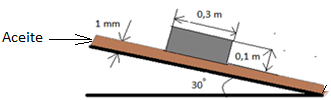
\includegraphics[width=0.6\linewidth]{imagenesEjercicios/bloqueDeslizantoT1}
		\caption{Esquema del bloque deslizando por el plano inclinado.}
		\label{fig:bloquedeslizantot1}
	\end{figure}
	\blue
	\[F_n=m g sen\alpha\]
	\[F_n=\rho V g sen\alpha\]
	\[\tau=\mu\dfrac{v}{e}=\dfrac{F_n}{S}=\rho h g sen\alpha\]
	\[
	\mu=
	\dfrac{e\rho h g sen\alpha}{v} =
	\dfrac{10^{-3}\,m\cdot1800\dfrac{kg}{m^3}\cdot0.1\,m\cdot 9.81 \dfrac{m}{s^2} \cdot sen(\ang{30})} {1\,m/s} = 
	0.8829\,Pa\cdot s\cdot\dfrac{1 P}{0.1\,Pa \cdot s}=8.83\,P
	\]
	\black
\end{enumerate}
\newpage

\section{Cinemática de la partícula fluida.}
\begin{enumerate}
	\item Dado el campo de velocidades de un flujo
	\[\vec{v}=4cos(\omega t)x\vec{i}-2cos(\omega t)y\vec{j}-2cos(\omega t)z\vec{k}\]
	\begin{enumerate}
		\item Indicar el tipo de flujo\\
		\textcolor{blue}{Flujo tridireccional, tridimensional y transitorio.}
		\item La ecuación de la trayectoria si en $t=0s$ se encuentra en $(x_0,y_0,z_0)$
		\[\textcolor{blue}{\vec{v}=\dfrac{d\vec{r}}{dt} \rightarrow \vec{r}=x\vec{i}+y\vec{j}+z\vec{k}}\]
		\[\textcolor{blue}{v_x=4cos(\omega t)x=\dfrac{dx}{dt}}\]
		\[\textcolor{blue}{v_y= -2cos(\omega t)y = \dfrac{dy}{dt}}\]
		\[\textcolor{blue}{v_z= -2cos(\omega t)z = \dfrac{dz}{dt}} \]
		\[\textcolor{blue}{\ln x|_0^t=\left.{\dfrac{4sen(\omega t)}{\omega}}\right |_0^t \rightarrow x=x_0 e^{\dfrac{4sen(\omega t)}{\omega}}}\]
		\[\textcolor{blue}{y=y_0 e^{\dfrac{-2sen(\omega t)}{\omega}}}\]
		\[\textcolor{blue}{z=z_0 e^{\dfrac{-2sen(\omega t)}{\omega}}}\]
		\item La ecuación de las sendas
		\[\textcolor{blue}{\ln \dfrac{x}{x_0}=\dfrac{4sen(\omega t)}{\omega}}\]
		\[\textcolor{blue}{\ln \dfrac{y}{y_0}=\dfrac{-2sen(\omega t)}{\omega}}\]
		\[\textcolor{blue}{\ln \dfrac{z}{z_0}=\dfrac{-2sen(\omega t)}{\omega}}\]
		\[\textcolor{blue}{\dfrac{1}{2}\ln \dfrac{x}{x_0}=-\ln \dfrac{y}{y_0} \rightarrow xy^2=x_0y_0^2}\]
		\[\textcolor{blue}{\ln \dfrac{z}{z_0}=\ln \dfrac{y}{y_0} \rightarrow yz_0=zy_0}\]
		\item Las líneas de corriente en un instante t
		\[\textcolor{blue}{\dfrac{dz}{v_z}=\dfrac{dy}{v_y}=\dfrac{dx}{v_x}}\]
		\[\textcolor{blue}{\dfrac{dy}{-2cos(\omega t)y}=\dfrac{dz}{-2cos(\omega t)z}\rightarrow \dfrac{dy}{y}=\dfrac{dz}{z}\rightarrow \ln z = \ln y + C_0 \rightarrow z=C_{00}y}\]
		\[\textcolor{blue}{\dfrac{dy}{-2cos(\omega t)y}=\dfrac{dx}{4cos(\omega t)x}\rightarrow -\dfrac{dy}{y}=\dfrac{dx}{2x}\rightarrow -\ln y = \dfrac{1}{2}\ln x + C_1 \rightarrow C_{11}=xy^2 }\]
	\end{enumerate}
	\newpage
	\item La velocidad de un fluido se encuentra definida por $\vec{v}=y\vec{j}+\left(ye^{-t}-z\right)\vec{k}$ Se pide:
	\begin{enumerate}
		\item Las componentes de la velocidad 
		\[\textcolor{blue}{v_x=0} \]
		\[	\textcolor{blue}{ v_y=y}\] 
			\[\textcolor{blue}{ v_z=ye^{-t} -z}\]
		\item Caracterización del flujo\\
		\textcolor{blue}{Flujo bidireccional, bidimensional y transitorio.}
		\item La aceleración de la partícula fluida cuando en t=0s pasa por el punto (0,1,0)
			\[\textcolor{blue}{a_L=\dfrac{\partial\vec{v}}{\partial t}=-ye^{-t}\vec{k}}\]
		\[\textcolor{blue}{a_c=\left(\vec{v}\cdot\vec{\nabla}\right)\vec{v}=
			\left(v_x\dfrac{\partial}{\partial x}
			+
			v_y\dfrac{\partial}{\partial y}
			+
			v_y\dfrac{\partial}{\partial z}
			\right)\cdot
			\left(v_x\vec{i}+v_y\vec{j}+v_z\vec{k}\right)		
		}\]
		\[\textcolor{blue}{a_c=\left(v_y\dfrac{\partial v_y}{\partial y} + v_z\dfrac{\partial v_y}{\partial z} \right)
			+\left(v_y\dfrac{\partial v_z}{\partial y} + v_z\dfrac{\partial v_z}{\partial z} \right)
			= y\vec{j}+z\vec{k}
		}\]
		\[	\textcolor{blue}{
			a_T=\dfrac{D\vec{v}}{Dt}=\dfrac{\partial\vec{v}}{\partial t}+\left(\vec{v}\cdot\vec{\nabla}\right)\vec{v}=a_L+a_c=y\vec{j}+\left(-ye^{-t}+z\right)\vec{k}
		}
		\]
	\[	\textcolor{blue}{
		\left.a_T \right|_{\vec{r}=(0,1,0)m,t=0s}=\vec{j}-\vec{k} \ \dfrac{m}{s^2}
	}
	\]
		\item Movimiento de la partícula fluida
				\setlength{\arraycolsep}{1.5pt}
		\renewcommand{\arraystretch}{2}
		\[\textcolor{blue}{\overline{\overline{\xi}}=\begin{bmatrix}
				\dfrac{\partial v_x}{\partial x} & \dfrac{1}{2}\left(\dfrac{\partial v_x}{\partial y}+\dfrac{\partial v_y}{\partial x}\right) &  \dfrac{1}{2}\left(\dfrac{\partial v_x}{\partial z}+\dfrac{\partial v_z}{\partial x}\right)\\
				\dfrac{1}{2}\left(\dfrac{\partial v_x}{\partial y}+\dfrac{\partial v_y}{\partial x}\right) & \dfrac{\partial v_y}{\partial y} &\dfrac{1}{2}\left(\dfrac{\partial v_y}{\partial z}+\dfrac{\partial v_z}{\partial y}\right)\\		
				\dfrac{1}{2}\left(\dfrac{\partial v_x}{\partial z}+\dfrac{\partial v_z}{\partial x}\right)  &\dfrac{1}{2}\left(\dfrac{\partial v_y}{\partial z}+\dfrac{\partial v_z}{\partial y}\right)& \dfrac{\partial v_z}{\partial z}\\	
			\end{bmatrix}=
			\begin{bmatrix}
				0 & 0 &  0\\
				0 & 1 &  \dfrac{e^{-t}}{2}\\
				0 &  \dfrac{e^{-t}}{2} &  -1\\	
			\end{bmatrix}
		}\]
		\setlength{\arraycolsep}{1.5pt}
		\renewcommand{\arraystretch}{2}
		\[\textcolor{blue}{\overline{\overline{\gamma}}=\begin{bmatrix}
				0 & \dfrac{1}{2}\left(\dfrac{\partial v_x}{\partial y}-\dfrac{\partial v_y}{\partial x}\right) &  \dfrac{1}{2}\left(\dfrac{\partial v_x}{\partial z}-\dfrac{\partial v_z}{\partial x}\right)\\
				-\dfrac{1}{2}\left(\dfrac{\partial v_x}{\partial y}-\dfrac{\partial v_y}{\partial x}\right) & 0 &\dfrac{1}{2}\left(\dfrac{\partial v_y}{\partial z}-\dfrac{\partial v_z}{\partial y}\right)\\		
				-\dfrac{1}{2}\left(\dfrac{\partial v_x}{\partial z}-\dfrac{\partial v_z}{\partial x}\right)  &-\dfrac{1}{2}\left(\dfrac{\partial v_y}{\partial z}-\dfrac{\partial v_z}{\partial y}\right)& 0\\	
			\end{bmatrix}=
			\begin{bmatrix}
				0 & 0 &  0\\
				0 & 0 &  -\dfrac{e^{-t}}{2}\\
				0 &  \dfrac{e^{-t}}{2} &  0\\	
			\end{bmatrix}
		}\]
		
		\item ¿Podría tratarse de un líquido?
			\[\textcolor{blue}{traza(\overline{\overline{\xi}})=1-1=0\rightarrow \text{Es un líquido.} }\]
		\item La velocidad de deformación lineal específica en la dirección del vector unitario $\vec{l}=\dfrac{1}{\sqrt{3}}\left(\vec{i}-\vec{j}+\vec{k}\right)$
		\[\textcolor{blue}{
			\overline{\overline{\xi}}\cdot\vec{n}=\begin{bmatrix}
				0 & 0 &  0\\
				0 & 1 &  \dfrac{e^{-t}}{2}\\
				0 &  \dfrac{e^{-t}}{2} &  -1\\	
			\end{bmatrix} \cdot \dfrac{1}{\sqrt{3}}\begin{bmatrix}
			1 \\
			-1 \\
			1 \\	
			\end{bmatrix}=\dfrac{1}{\sqrt{3}}\begin{bmatrix}
			0 \\
			-1+ \dfrac{e^{-t}}{2}\\
			-1-  \dfrac{e^{-t}}{2}\\	
			\end{bmatrix}
		}\]
	\end{enumerate}
	\item Considere el flujo definido por $v_y=z\left(t+2t^2\right)$ y $v_z=2y$. Determine:
	\begin{enumerate}
		\item Tipo de flujo\\
		\textcolor{blue}{Flujo bidireccional, bidimensional y transitorio.}
		\item La aceleración de la partícula fluida: total, local, convectiva y las contribuciones de la aceleración convectiva
	
			\[\textcolor{blue}{a_L=\dfrac{\partial\vec{v}}{\partial t}=z(1+4t)\vec{j}}\]
			\[\textcolor{blue}{a_c=\left(\vec{v}\cdot\vec{\nabla}\right)\vec{v}=
			\left(v_x\dfrac{\partial}{\partial x}
			+
		v_y\dfrac{\partial}{\partial y}
			+
		v_y\dfrac{\partial}{\partial z}
			\right)\cdot
			\left(v_x\vec{i}+v_y\vec{j}+v_z\vec{k}\right)		
			}\]
			
			\[\textcolor{blue}{a_c=\left(v_y\dfrac{\partial v_y}{\partial y} + v_z\dfrac{\partial v_y}{\partial z} \right)
				+\left(v_y\dfrac{\partial v_z}{\partial y} + v_z\dfrac{\partial v_z}{\partial z} \right)
				= 2y(t+2t^2)\vec{j}+2z(t+2t^2)\vec{k}
			}\]
			\[	\textcolor{blue}{
				a_T=\dfrac{D\vec{v}}{Dt}=\dfrac{\partial\vec{v}}{\partial t}+\left(\vec{v}\cdot\vec{\nabla}\right)\vec{v}=a_L+a_c=\left[z(1+4t)+2y(t+2t^2)\right]\vec{j}+2z(t+2t^2)\vec{k}
			}
			\]
			\[\textcolor{blue}{a_{c_v}=\vec{\nabla}\dfrac{|\vec{v}|^2}{2}=\dfrac{1}{2}\left[
				\dfrac{\partial}{\partial x}\left(v_x^2+v_y^2+v_z^2\right)\vec{i}
				+
				\dfrac{\partial}{\partial y}\left(v_x^2+v_y^2+v_z^2\right)\vec{j}
				+
				\dfrac{\partial}{\partial z}\left(v_x^2+v_y^2+v_z^2\right)\vec{k}
				\right]
			}\]
			\[\textcolor{blue}{a_{c_v}=
				4y\vec{j}+z\left(t^2+4t^3+4t^4\right)\vec{k}
			}\]
			\[\textcolor{blue}{a_{c_d}=-\vec{v} \times \left(\vec{\nabla}\times\vec{v}\right)=(\vec{v} \cdot\vec{\nabla})\vec{v}-\vec{\nabla}\dfrac{|\vec{v}|}{2}^2
			}\]
			\[\textcolor{blue}{a_{c_v}=\left[z(1+4t)+2y(t+2t^2)-4y\right]\vec{j}+z(2t+3t^2-4t^3-4t^4)\vec{k}}\]
		\item  El vector velocidad angular
		\[\textcolor{blue}{
			\vec{\omega}= \left(\vec{\nabla}\times\vec{v}\right)=
			\renewcommand{\arraystretch}{1.2}
			\begin{vmatrix}
				\vec i & \vec j & \vec k \\
				\dfrac{\partial}{\partial x} & \dfrac{\partial}{\partial y} & \dfrac{\partial}{\partial z} \\
				v_x & v_y & v_z \\
			\end{vmatrix}=
			\begin{vmatrix}
				\vec i & \vec j & \vec k \\
				0 & \dfrac{\partial}{\partial y} & \dfrac{\partial}{\partial z} \\
				0 & v_y & v_z \\
			\end{vmatrix}=
			\left[\dfrac{\partial v_z}{\partial y}-\dfrac{\partial v_y}{\partial z}\right]\vec{i}=\left(2-t-2t^2\right)\vec{i}
		}\]
		\item El movimiento de la partícula fluida
				\setlength{\arraycolsep}{1.5pt}
		\renewcommand{\arraystretch}{2}
			\[\textcolor{blue}{\overline{\overline{\xi}}=\begin{bmatrix}
				\dfrac{\partial v_x}{\partial x} & \dfrac{1}{2}\left(\dfrac{\partial v_x}{\partial y}+\dfrac{\partial v_y}{\partial x}\right) &  \dfrac{1}{2}\left(\dfrac{\partial v_x}{\partial z}+\dfrac{\partial v_z}{\partial x}\right)\\
				\dfrac{1}{2}\left(\dfrac{\partial v_x}{\partial y}+\dfrac{\partial v_y}{\partial x}\right) & \dfrac{\partial v_y}{\partial y} &\dfrac{1}{2}\left(\dfrac{\partial v_y}{\partial z}+\dfrac{\partial v_z}{\partial y}\right)\\		
				\dfrac{1}{2}\left(\dfrac{\partial v_x}{\partial z}+\dfrac{\partial v_z}{\partial x}\right)  &\dfrac{1}{2}\left(\dfrac{\partial v_y}{\partial z}+\dfrac{\partial v_z}{\partial y}\right)& \dfrac{\partial v_z}{\partial z}\\	
			\end{bmatrix}=
			\begin{bmatrix}
				0 & 0 &  0\\
				0 & 0 &  \dfrac{t+2t^2+2}{2}\\
				0 &  \dfrac{t+2t^2+2}{2} &  0\\	
			\end{bmatrix}
		}\]
	\setlength{\arraycolsep}{1.5pt}
	\renewcommand{\arraystretch}{2}
	\[\textcolor{blue}{\overline{\overline{\gamma}}=\begin{bmatrix}
			0 & \dfrac{1}{2}\left(\dfrac{\partial v_x}{\partial y}-\dfrac{\partial v_y}{\partial x}\right) &  \dfrac{1}{2}\left(\dfrac{\partial v_x}{\partial z}-\dfrac{\partial v_z}{\partial x}\right)\\
			-\dfrac{1}{2}\left(\dfrac{\partial v_x}{\partial y}-\dfrac{\partial v_y}{\partial x}\right) & 0 &\dfrac{1}{2}\left(\dfrac{\partial v_y}{\partial z}-\dfrac{\partial v_z}{\partial y}\right)\\		
			-\dfrac{1}{2}\left(\dfrac{\partial v_x}{\partial z}-\dfrac{\partial v_z}{\partial x}\right)  &-\dfrac{1}{2}\left(\dfrac{\partial v_y}{\partial z}-\dfrac{\partial v_z}{\partial y}\right)& 0\\	
		\end{bmatrix}=
		\begin{bmatrix}
			0 & 0 &  0\\
			0 & 0 &  \dfrac{t+2t^2+2}{2}\\
			0 &  \dfrac{-t-2t^2+2}{2} &  0\\	
		\end{bmatrix}
	}\]
		\item ¿Podría representar este campo de velocidades a un fluido que fuera un líquido?
		\[\textcolor{blue}{traza(\overline{\overline{\xi}})=0\rightarrow \text{Es un líquido.} }\]
	\end{enumerate}
	
	\item Un campo de velocidades viene dado por $v_x=x^2-2y^2; v_y=-2xy$
	$\textcolor{blue}{\Rightarrow \vec{v}=(x^2-2y^2)\vec{i}-2xy\vec{j}}$
	\begin{enumerate}
		\item Clasificación del flujo.\\
		\textcolor{blue}{Flujo bidireccional, bidimensional y estacionario.}
		\item La expresión de la aceleración total de la partícula fluida.
	
		\[	\textcolor{blue}{\dfrac{D\vec{v}}{Dt}=\dfrac{\partial\vec{v}}{\partial t}+\left(\vec{v}\cdot\vec{\nabla}\right)\vec{v}=\left(\vec{v}\cdot\vec{\nabla}\right)\vec{v}}\]
		
		\[\textcolor{blue}{\left(\vec{v}\cdot\vec{\nabla}\right)\vec{v}=v_x\dfrac{\partial}{\partial x}\left[v_x\vec{i}+v_y\vec{j}\right]+v_y\dfrac{\partial}{\partial y}\left[v_x\vec{i}+v_y\vec{j}\right]}\]
		
		\[\textcolor{blue}{\left(\vec{v}\cdot\vec{\nabla}\right)\vec{v}=\left[v_x\dfrac{\partial v_x}{\partial x} +v_y\dfrac{\partial v_x}{\partial y}\right]\vec{i}+\left[v_x\dfrac{\partial v_y}{\partial x} +v_y\dfrac{\partial v_y}{\partial y}\right]\vec{j}}\]
		
		\[\textcolor{blue}{\left(\vec{v}\cdot\vec{\nabla}\right)\vec{v}=\left[(x^2-2y^2)2x+4xy^2\right]\vec{i}+\left[(x^2-2y^2)(-2y)+4x^2y\right]\vec{j}}\]
		\[\textcolor{blue}{\left(\vec{v}\cdot\vec{\nabla}\right)\vec{v}=2\left(x^2+2y^2\right)\left(x\vec{i}+y\vec{j}\right)}\]
		\item Aceleración local.
		\[\textcolor{blue}{\dfrac{\partial \vec{v}}{\partial t}=0}\]
		\item Aceleración convectiva debida al cambio del módulo de la velocidad.
		\[\textcolor{blue}{\vec{\nabla}\dfrac{|\vec{v}|^2}{2}=\vec{\nabla}\left(\dfrac{v_x^2+v_y^2}{2}\right)=\vec{\nabla}\left(\dfrac{x^4+4y^4}{2}\right)=2x^3\vec{i}+8y^3\vec{j}}\]
		\item Aceleración convectiva debido al cambio de dirección de la velocidad.
			\[\textcolor{blue}{-\vec{v} \times \left(\vec{\nabla}\times\vec{v}\right)=(\vec{v} \cdot\vec{\nabla})\vec{v}-\vec{\nabla}\dfrac{|\vec{v}|}{2}^2=2\left(x^2+2y^2\right)\left(x\vec{i}+y\vec{j}\right)-\left(2x^3\vec{i}+8y^3\vec{j}\right)}\]
			\[\textcolor{blue}{-\vec{v} \times \left(\vec{\nabla}\times\vec{v}\right)=4y^2x\vec{i}+\left(2x^2y-4y^3\right)\vec{j}}\]
		\item Demostrar que la variación de la densidad a lo largo de una línea de corriente es nula.\\
		\textcolor{blue}{La variación de la densidad a lo largo de una línea de corriente nula $\Leftrightarrow$ fluido incompresible:}
		\[\textcolor{blue}{traza(\overline{\overline{\xi}})=\dfrac{\partial v_x}{\partial x}+\dfrac{\partial v_y}{\partial y}=2x-2x=0 \rightarrow \text{Fluido incompresible}}\]
		\item  Movimiento de la partícula fluida.
		
		\[\textcolor{blue}{\overline{\overline{\xi}}=\begin{bmatrix}
				\dfrac{\partial v_x}{\partial x} & \dfrac{1}{2}\left(\dfrac{\partial v_x}{\partial y}+\dfrac{\partial v_y}{\partial x}\right)\\
				\dfrac{1}{2}\left(\dfrac{\partial v_x}{\partial y}+\dfrac{\partial v_y}{\partial x}\right) & \dfrac{\partial v_y}{\partial y} \\				
		\end{bmatrix}=\begin{bmatrix}
		 2x & -3y\\
		 -3y& -2x \\				
		\end{bmatrix}
	}\]
	\[\textcolor{blue}{\overline{\overline{\gamma}}=\begin{bmatrix}
		0 & \dfrac{1}{2}\left(\dfrac{\partial v_x}{\partial y}-\dfrac{\partial v_y}{\partial x}\right) \\
		-\dfrac{1}{2}\left(\dfrac{\partial v_x}{\partial y}-\dfrac{\partial v_y}{\partial x}\right) & 0  \\
	\end{bmatrix}=\begin{bmatrix}
	0 & -y \\
	y & 0  \\
\end{bmatrix}}
\]

\[\textcolor{blue}{d\vec{v}=d\vec{r}\cdot\left(\overline{\overline{\xi}}+\overline{\overline{\gamma}}\right)=d\vec{r}\cdot\left(\begin{bmatrix}
		2x & -3y\\
		-3y& -2x \\				
	\end{bmatrix}+\begin{bmatrix}
		0 & -y \\
		y & 0  \\
	\end{bmatrix}\right)=d\vec{r}\cdot\begin{bmatrix}
		2x & -4y \\
		-2y & -2x  \\
	\end{bmatrix}}\]
	\end{enumerate}
\end{enumerate}
\newpage

\section{Conservación de la masa.}
\begin{enumerate}
	\item  Calcular la relación de velocidades entre el caudal de entrada y de salida en una tubería divergente
	\begin{figure}[H]

		\centering
		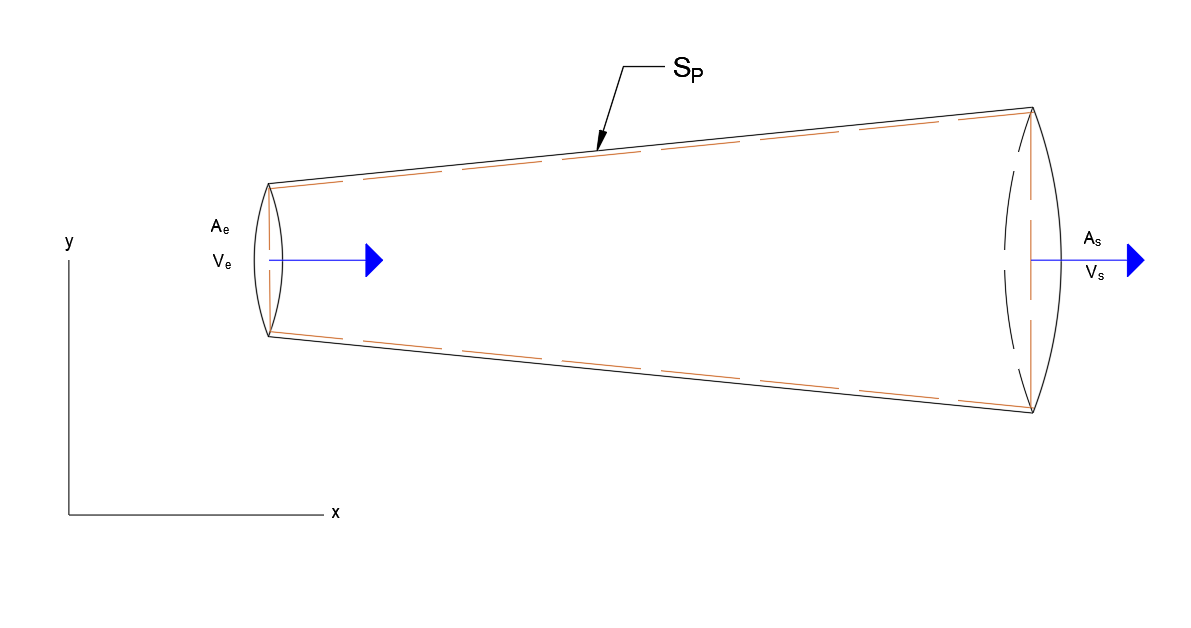
\includegraphics[width=0.7\linewidth]{imagenesEjercicios/tuberiaDivergente}
		\caption{Esquema de la tubería.}
		\label{fig:tuberiadivergente}

	\[\textcolor{blue}{\text{Se parte de la ecuación de conservación de la masa.}}\]
	\[\textcolor{blue}{\dfrac{d}{dt}\iiint_{V_c(t)}\rho\,dV+\oiint_{S_c(t)} \rho\left[(\vec{v}-\vec{v}_c)\cdot\vec{n}\right] \,dS=0}\]
\[\textcolor{blue}{
	\dfrac{d}{dt}\iiint_{V_c(t)}\rho\,dV=0 \rightarrow \text{El volumen no varia con el tiempo.}
}\]
\[\textcolor{blue}{
	\oiint_{S_c(t)} \rho\left[(\vec{v}-\vec{v}_c)\cdot\vec{n}\right] \,dS=
	\iint_{S_e(t)} \rho\left[(\vec{v}-\vec{v}_c)\cdot\vec{n}\right] \,dS+
	\iint_{S_p(t)} \rho\left[(\vec{v}-\vec{v}_c)\cdot\vec{n}\right] \,dS+
	\iint_{S_p(t)} \rho\left[(\vec{v}-\vec{v}_c)\cdot\vec{n}\right] \,dS
}\]
\[\textcolor{blue}{
	\iint_{S_e(t)} \rho\left[(\vec{v}-\vec{v}_c)\cdot\vec{n}\right] \,dS=-\rho v_e \iint_{S_e(t)}  \,dS=-\rho v_e A_e
}\]
\[\textcolor{blue}{
	\iint_{S_s(t)} \rho\left[(\vec{v}-\vec{v}_c)\cdot\vec{n}\right] \,dS=\rho v_s \iint_{S_s(t)}  \,dS=\rho v_s A_s
}\]
\textcolor{blue}{
	\[\iint_{S_p(t)} \rho\left[(\vec{v}-\vec{v}_c)\cdot\vec{n}\right] \,dS=0 \]
	 El volumen de control no se desplaza y el fluido  en contacto con las paredes tiene la misma velocidad que estas que al no moverse es 0.}

\textcolor{blue}{Por tanto:
\[-\rho v_e A_e+\rho v_s A_s=0\rightarrow v_e A_e=v_s A_s\]}
	\end{figure}
\newpage	
	\item Calcular la relación entre la velocidad de salida y la altura en un depósito con un agujero en su fondo
	\begin{figure}[H] 
		\centering
		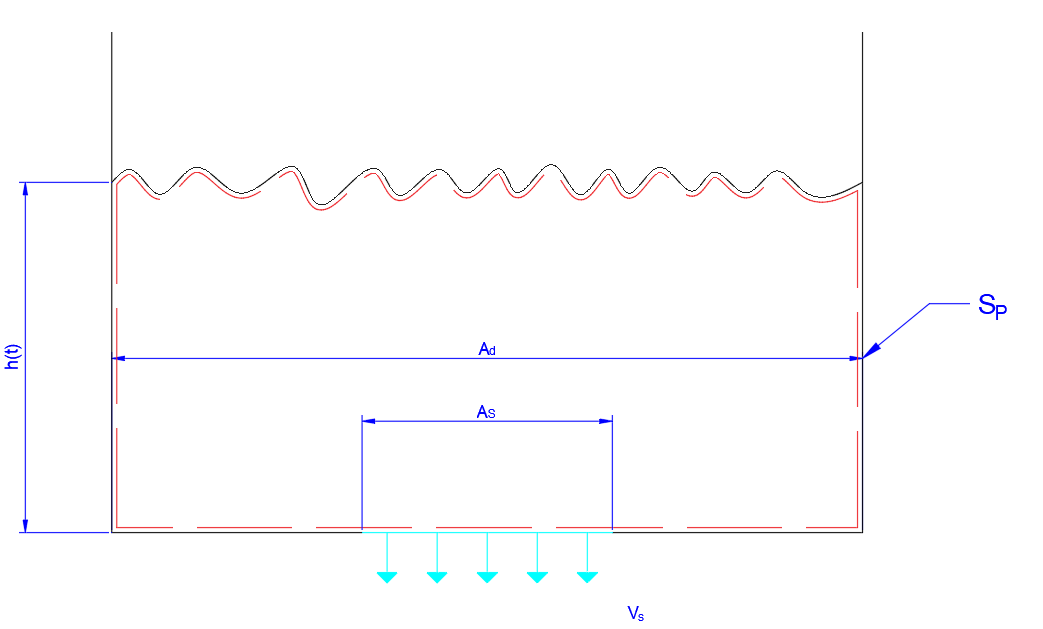
\includegraphics[width=0.7\linewidth]{imagenesEjercicios/depositoBujero}
		\caption{Esquema del depósito con el agujero en su fondo.}
		\label{fig:depositobujero}
	\[\textcolor{blue}{\text{Se parte de la ecuación de conservación de la masa.}}\]
\[\textcolor{blue}{\dfrac{d}{dt}\iiint_{V_c(t)}\rho\,dV+\oiint_{S_c(t)} \rho\left[(\vec{v}-\vec{v}_c)\cdot\vec{n}\right] \,dS=0}\]
\[\textcolor{blue}{
	\dfrac{d}{dt}\iiint_{V_c(t)}\rho\,dV=\rho \dfrac{d}{dt} V(t)=\rho A_d \dot{h}(t)
}\]
\[\textcolor{blue}{
	\oiint_{S_c(t)} \rho\left[(\vec{v}-\vec{v}_c)\cdot\vec{n}\right] \,dS=
	\iint_{S_s(t)} \rho\left[(\vec{v}-\vec{v}_c)\cdot\vec{n}\right] \,dS+
	\iint_{S_p(t)} \rho\left[(\vec{v}-\vec{v}_c)\cdot\vec{n}\right] \,dS+
	\iint_{S_n(t)} \rho\left[(\vec{v}-\vec{v}_c)\cdot\vec{n}\right] \,dS
}\]
\[\textcolor{blue}{
	\iint_{S_s(t)} \rho\left[(\vec{v}-\vec{v}_c)\cdot\vec{n}\right] \,dS=\rho v_s \iint_{S_s(t)}  \,dS=\rho v_s A_s
}\]
\[\textcolor{blue}{
	\iint_{S_n(t)} \rho\left[(\vec{v}-\vec{v}_c)\cdot\vec{n}\right] \,dS=0 \rightarrow \text{$v_c=v$ Y por tanto, se cancelan.}
}\]
\[\textcolor{blue}{
	\iint_{S_p(t)} \rho\left[(\vec{v}-\vec{v}_c)\cdot\vec{n}\right] \,dS=0
}\]
\textcolor{blue}{Por tanto:
	\[\rho A_d \dot{h}(t)+\rho v_s(t) A_s=0 \rightarrow A_d \dot{h}(t)+ v_s(t) A_s=0\]}
	\end{figure}
	
	\newpage
	\item Un envase que contiene aire comprimido se abre y el aire sale por el orificio con un gasto
	másico $\dot{m }$ = $C\rho$, donde $\rho$ es la densidad del aire del depósito y C es una constante. Se
	pide una expresión de la densidad en función del tiempo sabiendo que$\rho_0$ es la densidad
	inicial en el depósito y V su volumen, así como el tiempo necesario para que la densidad
	haya disminuido un 40 \%.
		\[\textcolor{blue}{\text{Se parte de la ecuación de conservación de la masa.}}\]
		\[\textcolor{blue}{\text{El volumen es constante y $\rho = f(t)$ con $\dot{m}=C\rho$}}\]
	\[\textcolor{blue}{\dfrac{d}{dt}\iiint_{V_c(t)}\rho\,dV+\oiint_{S_c(t)} \rho\left[(\vec{v}-\vec{v}_c)\cdot\vec{n}\right] \,dS=0}\]
	\[\textcolor{blue}{
		\dfrac{d}{dt}\iiint_{V_c(t)}\rho\,dV=V \dfrac{d}{dt} \rho(t)=V \dot{\rho}(t)
	}\]
	
	\textcolor{blue}{Como ya se ha hecho en los ejercicios anteriores, se descompone la superficie y como solo existe velocidad en el orificio:
	\[\oiint_{S_c(t)} \rho\left[(\vec{v}-\vec{v}_c)\cdot\vec{n}\right] \,dS=\rho v_s A_s = \dot{m}=C\rho\]	
	Por tanto:
	\[V \dot{\rho}(t)+C\rho(t)=0\]
	Que no es más que una EDO con variables separables cuya solución es:
	\[ln\left(\dfrac{\rho(t)}{\rho _0}\right)=-\dfrac{C}{V}t \rightarrow \text{Para una reducción de rho de un 40 \%} \rightarrow t=\dfrac{V}{C}ln\left(\dfrac{1}{0.6}\right)\]}
	\newpage
	\item Un tanque cilíndrico de diámetro (D) igual a 80 cm se comunica por el fondo con una
	tubería horizontal de diámetro (d) 15 cm por la que fluye agua. La
	velocidad del agua aguas arriba y aguas abajo del depósito es de 2,4 m/s y 1,8 m/s,
	respectivamente. En un instante de tiempo, la altura de agua (h) en el depósito es de 35
	cm. Calcular el tiempo que se necesita para rellenar el depósito que tiene una altura de
	1.2 m.
	\begin{figure}[H] 
		\centering
		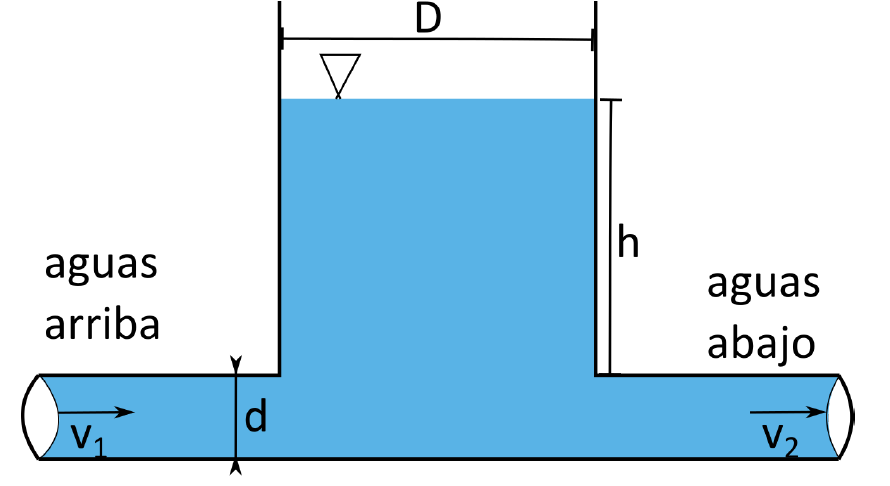
\includegraphics[width=0.7\linewidth]{imagenesEjercicios/tuberiaDeposito}
		\caption{Esquema de la tubería con el depósito.}
		\label{fig:tuberiadeposito}
	\end{figure}
	\textcolor{blue}{
	Se escoge como volumen de control el contorno del líquido, diferenciando entre 4 regiones:
	\begin{itemize}
		\item Entrada
		\item Salida
		\item Superficie depósito
		\item Pared
	\end{itemize}
	Partiendo de la ecuación de la masa y basandose en desarrollos anteriores:
	\[\dfrac{d}{dt}\iiint_{V_c(t)}\rho\,dV+\oiint_{S_c(t)} \rho\left[(\vec{v}-\vec{v}_c)\cdot\vec{n}\right] \,dS=0\]
	Como $\rho= cte$:
	\[\dfrac{d}{dt}\iiint_{V_c(t)}\,dV+\oiint_{S_c(t)} \left[(\vec{v}-\vec{v}_c)\cdot\vec{n}\right] \,dS=0\]
	\[\dfrac{d}{dt}\left[\pi \dfrac{D^2}{4}h(t)+l_{H}\pi\dfrac{d^2}{4}\right]-v_e\pi\dfrac{d^2}{4}+v_s\pi\dfrac{d^2}{4}=0\]
	\[D^2\dot{h}(t)-v_e d^2+v_s d^2=0\]
	Resolviendo la EDO
	\[h(t)=h_0+\dfrac{d^2}{D^2}\left(v_e-v_s\right) t\rightarrow \text{Sustituyendo los datos del enunciado se obtiene} \rightarrow t=40.3s\]
	}
	\newpage
	\item Se dispone de un émbolo de diámetro ($D_c$) con su superficie perforada con N agujeros de
	diámetro d que se disponen equidistantes al centro. Inicialmente el cilindro
	se encuentra lleno de un fluido incompresible de densidad $\rho$. El émbolo se desplaza con
	una velocidad $w_0$, produciéndose la salida del fluido con velocidad $v_s$ por un orificio de
	diámetro $D_s$. Se pide calcular la velocidad $v_s$ en función de los datos del ejercicio.
	\begin{figure}[H] 
		\centering
		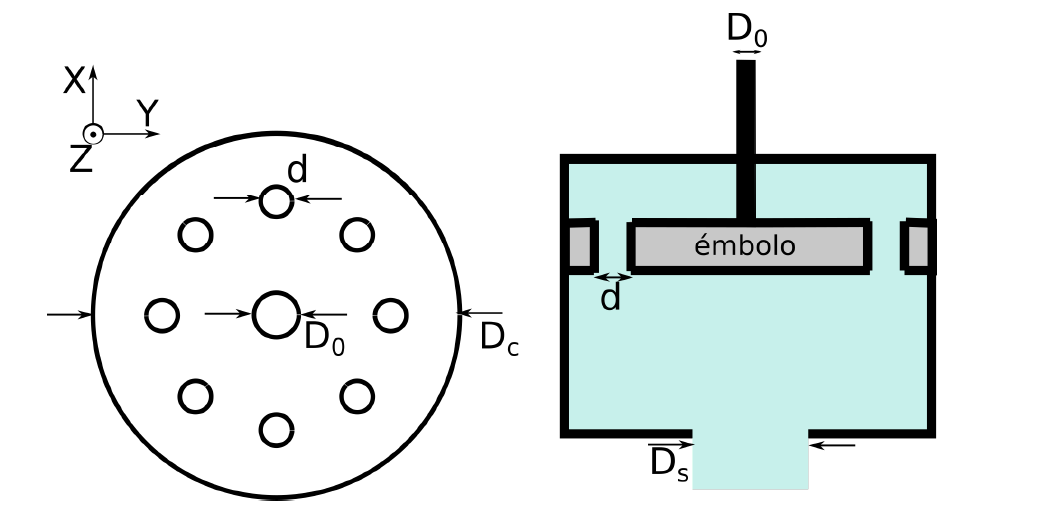
\includegraphics[width=0.7\linewidth]{imagenesEjercicios/emboloPerforado}
		\caption{Esquema del émbolo Perforado.}
		\label{fig:emboloperforado}

	\end{figure}
	\textcolor{blue}{
		Se escoge el volumen de control marcado sobre la figura y se plantea la ecuación de conservación de la masa:
	\[\dfrac{d}{dt}\iiint_{V_c(t)}\rho\,dV+\oiint_{S_c(t)} \rho\left[(\vec{v}-\vec{v}_c)\cdot\vec{n}\right] \,dS=0\]
	Como $\rho=cte$:
	\[\dfrac{d}{dt}\iiint_{V_c(t)}\,dV+\oiint_{S_c(t)} \left[(\vec{v}-\vec{v}_c)\cdot\vec{n}\right] \,dS=0\]
	El término local, como la única variación del volumen ocurre por la introducción de la varilla:
	\[\dfrac{d}{dt}\iiint_{V_c(t)}\,dV=-\omega _0 \pi \dfrac{D^2_0}{4}\]
	El término convectivo, teniendo en cuenta que las superficies son la pared o la de salida:
	\[\oiint_{S_c(t)} \left[(\vec{v}-\vec{v}_c)\cdot\vec{n}\right] \,dS=v_s \pi \dfrac{D^2_s}{4}\]
	Por tanto:
	\[-\omega _0 \pi \dfrac{D^2_0}{4}+v_s \pi \dfrac{D^2_s}{4}=0\rightarrow v_s=\omega _0 \left(\dfrac{D_0}{D_s}\right)^2\]
	}	
	
	\newpage
	\item Calcular en función de la altura la relación con la velocidad de un depósito con varios agujeros
	\begin{figure}[H]
		\centering
		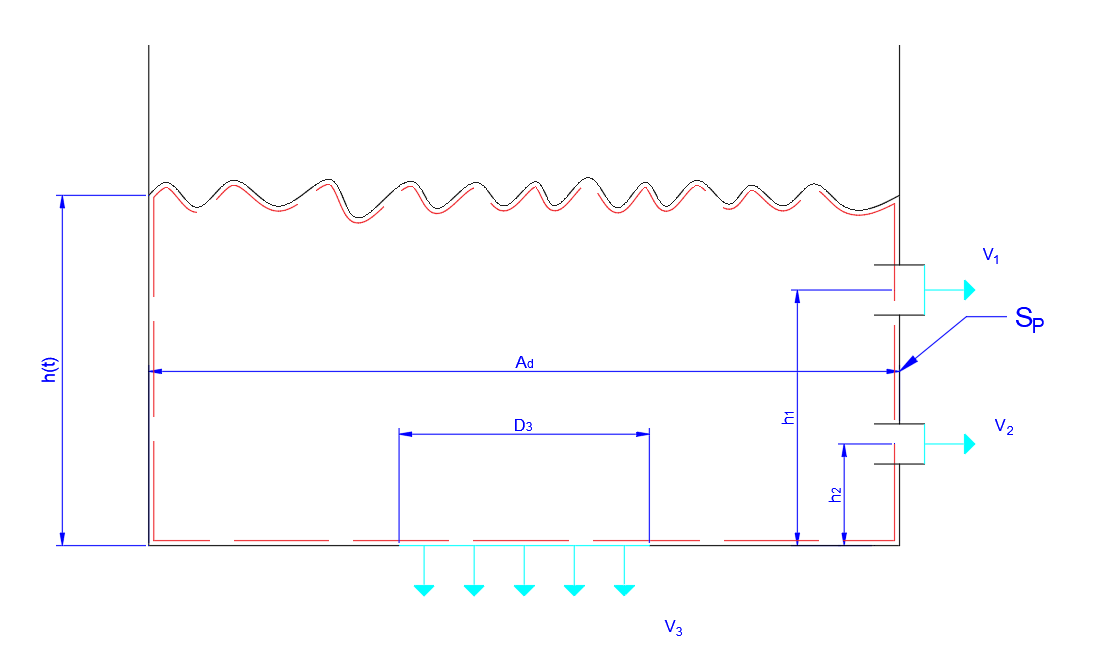
\includegraphics[width=0.7\linewidth]{imagenesEjercicios/depositoVariosBujeros}
		\caption{Esquema del depósito con varios agujeros.}
		\label{fig:depositovariosbujeros}
	\end{figure}
\textcolor{blue}{
Teniendo en cuenta los resultados obtenidos anteriormente para un depósito, se pueden plantear directamente las ecuaciones teniendo en cuenta las distintas regiones:
\begin{itemize}
	\item $h(t)>h_1$
	\[-A_d\dot{h}(t)=v_3\dfrac{\pi D^2_3}{4}+v_2\dfrac{\pi D^2_2}{4}+v_1\dfrac{\pi D^2_1}{4}\]
	\item $h_1>h(t)>h_2$
	\[-A_d\dot{h}(t)=v_3\dfrac{\pi D^2_3}{4}+v_2\dfrac{\pi D^2_2}{4}\]
	\item $h(t)<h_2$
	\[-A_d\dot{h}(t)=v_3\dfrac{\pi D^2_3}{4}\]
\end{itemize}
}

	\newpage
	\item El flujo de un fluido está representado por el siguiente campo de velocidades: u = u (x, t);
	v = 0; w = 0, y densidad $\rho$ =  $\rho _0$ [a - cos ($\omega$t)] con a$>$1. Determinar la función v (x, t)
	sabiendo que v (0, t) = $v_0$.
	\textcolor{blue}{
	\[\rho =  \rho _0 [a - cos (\omega t)] \ y \ v=f(x,t)\]
	Se plantea la ecuación de conservación de la masa en forma diferencial:
	\[\dfrac{\partial \rho}{\partial t} +\vec{\nabla}\cdot\left(\rho\vec{v}\right)=0\]
	\[\dfrac{\partial}{\partial t}\left(\rho _0 [a - cos (\omega t)]\right)+\left[\dfrac{\partial}{\partial x}\vec{i}+
	\dfrac{\partial}{\partial y}\vec{j}+
	\dfrac{\partial}{\partial z}\vec{k}\right]\cdot \left[ \rho _0 [a - cos (\omega t)] \right]v(x,t)=0\]
	\[
	\omega \rho _0 sen(\omega t)+\left[ \rho _0 [a - cos (\omega t)] \right]\dfrac{\partial}{\partial x}v(x,t)=0
	\]
	\[\dfrac{\partial}{\partial x}v(x,t)=-\dfrac{\omega sen(\omega t)}{a - cos (\omega t)}\]
	Resolviendo la EDO con la condición de que v (0, t) = $v_0$.
	\[v(x,t)=-\dfrac{\omega sen(\omega t)}{a - cos (\omega t)}x+v_0\]
	}
\end{enumerate}
\newpage

\section{Conservación de la cantidad de movimiento.}
\begin{enumerate}
	\item Considérese una tubería de sección decreciente con un codo con un ángulo $\alpha$. Calcule la fuerza que se ejerce sobre las paredes.
	\begin{figure}[H]
		\centering
		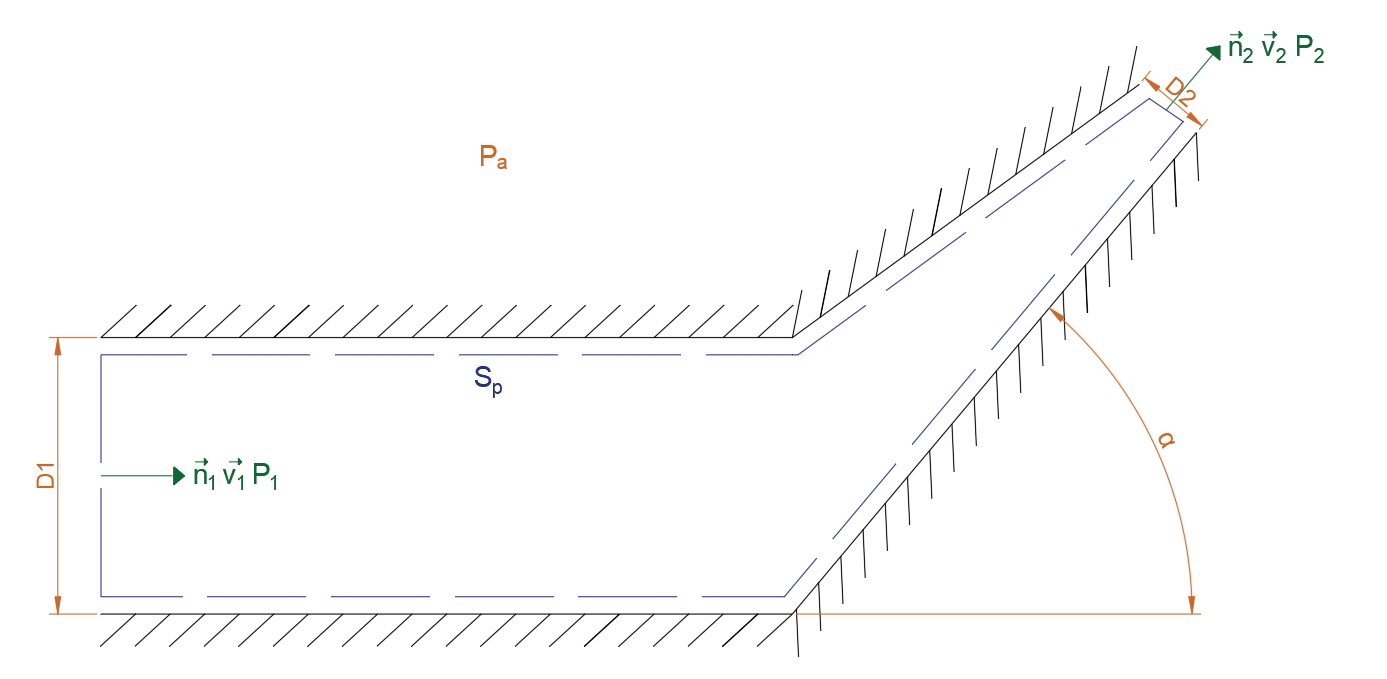
\includegraphics[width=0.7\linewidth]{imagenesEjercicios/tuberiaCodoDecreciente}
		\caption{Esquema de la tubería.}
		\label{fig:tuberiacododecreciente}
	\end{figure}
	\textcolor{blue}{
	Se plantea la ecuación de conservación de la masa:  
	\[\dfrac{d}{dt}\iiint_{V_c}\rho\,dV+\oiint_{S_c} \rho\left[(\vec{v}-\vec{v}_c)\cdot\vec{n}\right] \,dS=0\]
	Como el fluido es globalmente estacionario y no varia el volumen:
	\[\rho\oiint_{S_c} \left[(\vec{v}-\vec{v}_c)\cdot\vec{n}\right] \,dS=0\]
	\[\oiint_{S_c} \left[(\vec{v}-\vec{v}_c)\cdot\vec{n}\right] \,dS=
	\iint_{S_1} \left[(\vec{v}-\vec{v}_c)\cdot\vec{n}\right] \,dS
	+
	\iint_{S_2} \left[(\vec{v}-\vec{v}_c)\cdot\vec{n}\right] \,dS
	+
	\iint_{S_p} \left[(\vec{v}-\vec{v}_c)\cdot\vec{n}\right] \,dS\]
	\[\iint_{S_1} \left[(\vec{v}-\vec{v}_c)\cdot\vec{n}\right] \,dS=-v_1\pi\dfrac{D_1^2}{4}\]
	\[\iint_{S_2} \left[(\vec{v}-\vec{v}_c)\cdot\vec{n}\right] \,dS=v_2\pi\dfrac{D_2^2}{4}\]
	\[\iint_{S_p} \left[(\vec{v}-\vec{v}_c)\cdot\vec{n}\right] \,dS=0\]
	Por tanto de la conservación de la masa se obtiene:
	\[v_1D_1^2=v_2D_2^2\]
	Planteando la conservación de la cantidad de movimiento
	\[\iiint_{V_c}\vec{f}_V\,dV
	+
	\oiint_{S_c}\left(-P\overline{\overline{I}}+\overline{\overline{\tau}}\right)\cdot\vec{n}\,dS=
	\iiint_{V_c}\dfrac{\partial \rho\vec{v}}{\partial t}\,dV
	+\oiint_{S_c}\rho\vec{v}\left[\left(\vec{v}-\vec{v}_c\right)\cdot\vec{n}\right]\,dS\]
	El término de fuerzas volumétricas:
	\[\iiint_{V_c}\vec{f}_V\,dV=\iiint_{V_f}\rho\vec{g}\,dV=\rho \vec{g}V_c\]
	El término de fuerzas superficiales:
	\[\oiint_{S_c}\left(-P\overline{\overline{I}}+\overline{\overline{\tau}}\right)\cdot\vec{n}\,dS=
	\iint_{S_1}\left(-P\overline{\overline{I}}+\overline{\overline{\tau}}\right)\cdot\vec{n}\,dS
	+
	\iint_{S_2}\left(-P\overline{\overline{I}}+\overline{\overline{\tau}}\right)\cdot\vec{n}\,dS
	+
	\iint_{S_p}\left(-P\overline{\overline{I}}+\overline{\overline{\tau}}\right)\cdot\vec{n}\,dS
	\]
	\begin{itemize}
		\item 	Como se cumple que la fuerza ejercida por la atmósfera sobre toda la superficie de control es nula:
		\[\oiint_{S_c}P_a\vec{n}\,dS=0\]
		\item Por tanto, para tener en cuenta las aportaciones de fuerza tanto del fluido como de la presión atmosférica:
		\[\oiint_{S_c}\left(-P\overline{\overline{I}}+\overline{\overline{\tau}}\right)\cdot\vec{n}\,dS=\oiint_{S_c}\left[-(P-P_a)\overline{\overline{I}}+\overline{\overline{\tau}}\right]\cdot\vec{n}\,dS\]
		\item Además, el término de fuerza superficial sobre las paredes es la fuerza a calcular:
		\[\iint_{S_p}\left[-(P-P_a)\overline{\overline{I}}+\overline{\overline{\tau}}\right]\cdot\vec{n}\,dS=-F_{fluido+atm\rightarrow pared}\]
		\item En un perfil uniforme se cumple que $\tau_v$ es despreciable frente al término de presión. Por tanto:
		\[\oiint_{S_c}\left(-P\overline{\overline{I}}+\overline{\overline{\tau}}\right)\cdot\vec{n}\,dS=
		\iint_{S_1}-(P-P_a)\vec{n}\,dS
		+
		\iint_{S_2}-(P-P_a)\vec{n}\,dS
		-F_{fluido\rightarrow pared}\]
		\[\oiint_{S_c}\left(-P\overline{\overline{I}}+\overline{\overline{\tau}}\right)\cdot\vec{n}\,dS=
		-(P_1-P_a)\dfrac{\pi D^2_1}{4}(-\vec{i})
		-(P_2-P_a)\dfrac{\pi D^2_2}{4}(\vec{n})
		-F_{fluido+atm\rightarrow pared}\]
		\[\oiint_{S_c}\left(-P\overline{\overline{I}}+\overline{\overline{\tau}}\right)\cdot\vec{n}\,dS=
		\dfrac{\pi}{4}\left[(P_1-P_a) D^2_1\vec{i}-(P_2-P_a)D^2_2\left(cos(\alpha)\vec{i}+sen(\alpha)\vec{j}\right)\right]
		-F_{fluido+atm\rightarrow pared}\]
	\end{itemize}
	El término local:
	\[\iiint_{V_c}\dfrac{\partial \rho\vec{v}}{\partial t}\,dV=0\]
	El término convectivo:
	\[\oiint_{S_c}\rho\vec{v}\left[\left(\vec{v}-\vec{v}_c\right)\cdot\vec{n}\right]\,dS=
	\iint_{S_1}\rho\vec{v}\left[\left(\vec{v}-\vec{v}_c\right)\cdot\vec{n}\right]\,dS+
	\iint_{S_2}\rho\vec{v}\left[\left(\vec{v}-\vec{v}_c\right)\cdot\vec{n}\right]\,dS
	+\iint_{S_p}\rho\vec{v}\left[\left(\vec{v}-\vec{v}_c\right)\cdot\vec{n}\right]\,dS\]
	\[\iint_{S_1}\rho\vec{v}\left[\left(\vec{v}-\vec{v}_c\right)\cdot\vec{n}\right]\,dS=\rho v_1\vec{i}\cdot v_1\vec{i}\cdot-\vec{i}\dfrac{D^2_1}{\pi}=-\rho v^2_1\dfrac{D^2_1}{\pi}\vec{i}\]
	\[\iint_{S_2}\rho\vec{v}\left[\left(\vec{v}-\vec{v}_c\right)\cdot\vec{n}\right]\,dS=\rho v_2\vec{n}\cdot v_2\vec{n}\cdot\vec{n}\dfrac{D^2_2}{\pi}=\rho v^2_2\dfrac{D^2_2}{\pi}\vec{n}=\rho v^2_2\dfrac{D^2_2}{\pi}\left[cos(\alpha)\vec{i}+sen(\alpha)\vec{j}\right]\]
	\[\iint_{S_p}\rho\vec{v}\left[\left(\vec{v}-\vec{v}_c\right)\cdot\vec{n}\right]\,dS=0\]
	Por tanto, sustituyendo los término se obtiene:
	\[F_{fluido+atm\rightarrow pared}=\dfrac{\pi}{4}\left[(P_1-P_a) D^2_1\vec{i}-(P_2-P_a)D^2_2\vec{n}\right]+\rho g V_c \vec{j}
	+\rho\dfrac{\pi}{4}\left[v^2_1D^2_1\vec{i}-v^2_2D^2_2\vec{n}\right] \]
	\[\vec{n}=cos(\alpha)\vec{i}+sen(\alpha)\vec{j}\]
	}
		
	
	
	\newpage
	
	\item Se tiene un elemento de área de 2 $mm^2$ cuya normal es paralela al vector de componentes
	(1, 2, 3). Si el tensor de esfuerzos es de la forma $\tau_{xx} = -2 \times 10^5; \tau_{yy} = -110 \times 10^ 3; \tau_{zz} =
	-115 \times 10^3; \tau_{xy} = 1\times10^3; \tau_{xz} = -5 \times 10^4;  \tau_{zy} = 1 \times 10^5$, todos ellos en pascales. Se pide:
	\begin{itemize}
		\item 	El tensor de esfuerzos
		\textcolor{blue}{
		\[\overline{\overline{\tau}}=\begin{bmatrix}
			\tau_{xx} &\tau_{xy}&\tau_{xz}\\
				\tau_{yx} &\tau_{yy}&\tau_{yz}\\
					\tau_{zx} &\tau_{zy}&\tau_{zz}\\
		\end{bmatrix}=
		\begin{bmatrix}
		 -2 \times 10^5&1\times10^3&-5 \times 10^4\\
		1\times10^3& -110 \times 10^ 3&1 \times 10^5\\
		 -5 \times 10^4&1 \times 10^5&-115 \times 10^3\\
		\end{bmatrix}
		\]}
		\item El valor de la fuerza superficial sobre dicha área  si la presión es de 1.5 bares.
			\textcolor{blue}{\[F=\oiint_{S_c}\left(-p\overline{\overline{I}}+\overline{\overline{\tau}}\right)\cdot\vec{n}\,dS=\left(-p\overline{\overline{I}}+\overline{\overline{\tau}}\right)\cdot\vec{n}S \]
			\[	F=-1.5\times10^5 \dfrac{2\times 10^{-6}}{\sqrt{1^2+2^2+3^2}}\begin{bmatrix}
					1 \\
					2 \\
					3 \\
				\end{bmatrix}+	\begin{bmatrix}
				-2 \times 10^5&1\times10^3&-5 \times 10^4\\
				1\times10^3& -110 \times 10^ 3&1 \times 10^5\\
				-5 \times 10^4&1 \times 10^5&-115 \times 10^3\\
				\end{bmatrix}\cdot\dfrac{2\times 10^{-6}}{\sqrt{1^2+2^2+3^2}}\begin{bmatrix}
				1 \\
				2 \\
				3 \\
				\end{bmatrix}\]
			\[F=\dfrac{1}{\sqrt{14}}\begin{bmatrix}
				-0.996 \\
				-0.438 \\
				-1.29 \\
			\end{bmatrix}\]}
	\end{itemize}
\newpage
	

	\item Considérese un depósito cilíndrico de sección A que se encuentra fijo sobre una plataforma. El depósito tiene una altura h de agua y en el instante inicial se practica
	un orificio de área $A_s$ en la parte inferior de la pared. ¿Hacia dónde tendería a desplazarse
	si no estuviera fijado a la plataforma? Calcular la fuerza de reacción de la plataforma sobre
	el depósito.
 \begin{figure}[H]
 	\centering
 	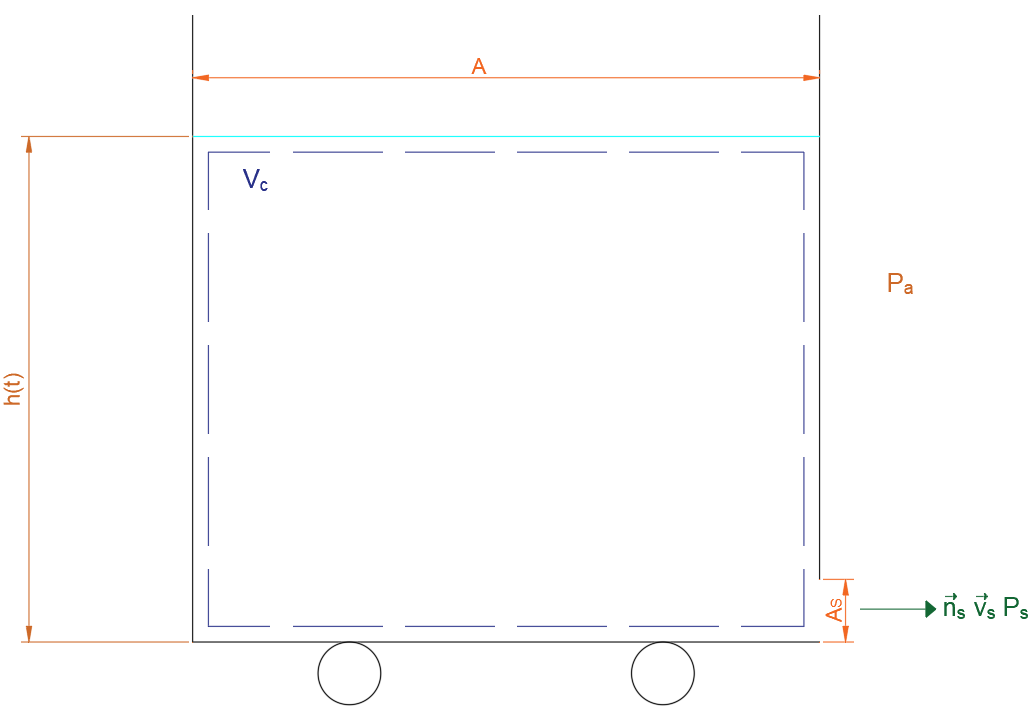
\includegraphics[width=0.7\linewidth]{imagenesEjercicios/depositobloqueado}
 	\caption{Esquema del depósito.}
 	\label{fig:depositobloqueado}
 \end{figure}
 \textcolor{blue}
 {
 	Se plantea la ecuación de conservación de la masa: 
 	\[\dfrac{d}{dt}\iiint_{V_c}\rho\,dV+\oiint_{S_c} \rho\left[(\vec{v}-\vec{v}_c)\cdot\vec{n}\right] \,dS=0\]
 	Teniendo en cuenta desarrollos de ejercicios anteriores:
 	\[A\dot{h}(t)=v_s(t)A_s\]
 	Planteando la conservación de la cantidad de movimiento, donde solo se buscan los términos en dirección $\vec{i}$ ya que el depósito si no estuviese fijo se movería hacia la izquierda y los términos de fuerza en dirección al suelo solo soportan el peso del depósito y no intervendrían en este ''movimiento''
 	\[\iiint_{V_c}\vec{f}_V\,dV
 	+
 	\oiint_{S_c}\left(-P\overline{\overline{I}}+\overline{\overline{\tau}}\right)\cdot\vec{n}\,dS=
 	\iiint_{V_c}\dfrac{\partial \rho\vec{v}}{\partial t}\,dV
 	+\oiint_{S_c}\rho\vec{v}\left[\left(\vec{v}-\vec{v}_c\right)\cdot\vec{n}\right]\,dS\]
 	El término de fuerzas volumétricas es nulo en la dirección de la fuerza a reacción a calcular:
 	\[\iiint_{V_c}\vec{f}_V\,dV=0\]
 	El término de fuerzas superficiales:
 	\[\oiint_{S_c}\left(-P\overline{\overline{I}}+\overline{\overline{\tau}}\right)\cdot\vec{n}\,dS=
 	\iint_{S_s}\left(-P\overline{\overline{I}}+\overline{\overline{\tau}}\right)\cdot\vec{n}\,dS
 	+
 	\iint_{S_n}\left(-P\overline{\overline{I}}+\overline{\overline{\tau}}\right)\cdot\vec{n}\,dS
 	+
 	\iint_{S_p}\left(-P\overline{\overline{I}}+\overline{\overline{\tau}}\right)\cdot\vec{n}\,dS
 	\]
 	\begin{itemize}
 		\item En un perfil uniforme se cumple que $\tau_v$ es despreciable frente al término de presión. Por tanto la resultante en la dirección $\vec{i}$:
 		\[\oiint_{S_c}\left(-P\overline{\overline{I}}+\overline{\overline{\tau}}\right)\cdot\vec{n}\,dS\cdot\vec{i}=
 		\left[
 		\iint_{S_s}-(P-P_a)\vec{n}\,dS
 		+
 		\iint_{S_n}-(P-P_a)\vec{n}\,dS
 		+
 		\iint_{S_p}-(P-P_a)\vec{n}\,dS
 		\right]\cdot\vec{i}
 		\]
 		\[\oiint_{S_c}\left(-P\overline{\overline{I}}+\overline{\overline{\tau}}\right)\cdot\vec{n}\,dS\cdot\vec{i}=
 		(P_s-P_a)A_s
 		+0
 		-F_{fl+atm\rightarrow dep}=(P_s-P_a)A_s -F_{fl+atm\rightarrow dep}\]
 	\end{itemize}
 	El término local es nulo debido a que la variación de la derivada de la altura tiene un orden de magnitud mucho menor al resto de términos y, por tanto es despreciable :
 	\[\iiint_{V_c}\dfrac{\partial \rho\vec{v}}{\partial t}\,dV=0\]
 	El término convectivo en la dirección de $\vec{i}$:
 	\[\oiint_{S_c}\rho\vec{v}\left[\left(\vec{v}-\vec{v}_c\right)\cdot\vec{n}\right]\,dS=
 	\iint_{S_n}\rho\vec{v}\left[\left(\vec{v}-\vec{v}_c\right)\cdot\vec{n}\right]\,dS+
 	\iint_{S_s}\rho\vec{v}\left[\left(\vec{v}-\vec{v}_c\right)\cdot\vec{n}\right]\,dS
 	+\iint_{S_p}\rho\vec{v}\left[\left(\vec{v}-\vec{v}_c\right)\cdot\vec{n}\right]\,dS\]
 	\[\oiint_{S_c}\rho\vec{v}\left[\left(\vec{v}-\vec{v}_c\right)\cdot\vec{n}\right]\,dS\cdot\vec{i}=
 	0+
 	\rho v^2_s A_s \vec{i}\cdot\vec{i}
 	+0=	\rho v^2_s A_s\]
 	Por tanto, sustituyendo los término se obtiene:
	 \[(P_s-P_a)A_s -F_{fl+atm\rightarrow dep}=\rho v^2_s A_s\rightarrow P_s=P_a\]
	 \[|F_{fl+atm\rightarrow dep}|=|\rho v^2_s A_s|\rightarrow  \text{Como se mueve a la izquierda: } \vec{F}_{fl+atm\rightarrow dep}= -\rho v^2_s A_s\vec{i}\]
	 Para obtener la relación entre altura y velocidad de salida se aplica el teorema de Bernouilli entre la parte superior del depósito y la salida:
	 \[P_1+\rho g h(t)=P_s+\dfrac{v^2_s(t)}{2}\rho\rightarrow P_1=P_s=P_a \rightarrow h(t)=\dfrac{v^2_s(t)}{2g}\rightarrow v_s(t)=\sqrt{2gh(t)}\]
	 Aplicando esta expresión junto a la obtenida con la conservación de la masa:
	 \[v_s(t)=\sqrt{2gh(t)}\]
	 \[A\dot{h}(t)=v_s(t)A_s\]
	 Resolviendo la EDO se obtiene:
	 \[\sqrt{h(t)}=\dfrac{-A_s}{A}\sqrt{\dfrac{g}{2}}t+\sqrt{h_0}\]
}
%\item Considérese el siguiente chorro impactando contra una placa de forma axilsimétrica.
%
%\begin{figure}[H]
%	\centering
%		\begin{circuitikz}
%			\tikzstyle{every node}=[font=\large]
%			\draw  (-5.5,15.75) rectangle (-3.25,15.25);
%			\draw  (-5.5,13.25) rectangle (-3.25,12.75);
%			\draw [ color={rgb,255:red,0; green,128; blue,255}, short] (-3.25,15.25) -- (0,15.25);
%			\draw [ color={rgb,255:red,0; green,128; blue,255}, short] (0,15.25) .. controls (1,15.25) and (1.25,15.5) .. (1.25,16.5);
%			\draw [ color={rgb,255:red,0; green,128; blue,255}, short] (1.25,16.5) -- (1.25,18.5);
%			\draw [ color={rgb,255:red,0; green,128; blue,255}, short] (-3.25,13.25) -- (0,13.25);
%			\draw [ color={rgb,255:red,0; green,128; blue,255}, short] (0,13.25) .. controls (1.25,13.25) and (1.25,13) .. (1.25,12);
%			\draw [ color={rgb,255:red,0; green,128; blue,255}, short] (1.25,12) -- (1.25,10);
%			\draw [short] (1.5,18.5) -- (1.5,10);
%			\draw [short] (2.5,18.5) -- (2.5,10);
%			\draw [ color={rgb,255:red,0; green,128; blue,0}, -latex] (2,14.25) -- (2,15.75)node[pos=1,above]{$\vec{e}_r$};
%			\draw [-latex] (2,14.25) -- (4.5,14.25)node[pos=1,right]{$\vec{v}_p$};
%			\draw [ color={rgb,255:red,0; green,128; blue,0}, -latex] (2,14.25) -- (3.25,14.25)node[pos=1,above]{$\vec{k}$};
%			\draw [short] (-6,14.25) -- (-5,14.25);
%			\draw [short] (-4.75,14.25) -- (-4.5,14.25);
%			\draw [short] (-4.25,14.25) -- (-3.25,14.25);
%			\draw [short] (-3,14.25) -- (-2.75,14.25);
%			\draw [short] (-2.5,14.25) -- (-1.5,14.25);
%			\draw [short] (-1.25,14.25) -- (-1,14.25);
%			\draw [short] (-0.75,14.25) -- (0.25,14.25);
%			\draw [short] (0.5,14.25) -- (0.75,14.25);
%			\draw [short] (1,14.25) -- (2,14.25);
%			\draw [ color={rgb,255:red,255; green,0; blue,0}, -latex] (-5.5,14.75) -- (-3.5,14.75)node[pos=1,right]{$\vec{v}_e$};
%			\node [font=\large, color={rgb,255:red,0; green,128; blue,255}] at (-1.75,13.75) {$\rho=cte$};
%			\node [font=\large] at (-4.25,17.75) {$P_a$};
%			\draw [-latex] (0.75,17.75) -- (1.25,17.75)node[pos=0,above]{h(r)};
%			\draw [-latex] (2,17.75) -- (1.5,17.75);
%			\node [font=\large] at (1,15.25) {\textbf{r}};
%			\draw [-latex] (-5.5,9.75) -- (-4.25,9.75)node[pos=1,right]{$\vec{i}$};
%			\draw [-latex] (-5.5,9.75) -- (-5.5,11)node[pos=1,above]{$\vec{j}$};
%			\draw [ color={rgb,255:red,128; green,0; blue,255}, -latex] (1.25,11.75) -- (2.25,11.75)node[pos=0.5,above]{$\vec{n}_p$};
%			\draw [ color={rgb,255:red,128; green,0; blue,255}, -latex] (1,15.5) -- (0.25,16.25)node[pos=1,above]{$\vec{n}_{int}$};
%			\draw [ color={rgb,255:red,128; green,0; blue,255}, -latex] (-4.5,13.75) -- (-5.75,13.75)node[pos=0.4,above]{$\vec{n}_e$};
%			\draw [ color={rgb,255:red,128; green,0; blue,255}, -latex] (1.5,11.25) -- (1.5,10.25)node[pos=0.5,left]{$\vec{n}_r,$ $\vec{v}_r$};
%			\draw [ color={rgb,255:red,0; green,128; blue,255}, dashed] (-4.5,15.25) -- (-4.5,13.25);
%			\node [font=\large, color={rgb,255:red,0; green,128; blue,255}] at (0.25,13.75) {$V_C$};
%			\node [font=\large] at (-4.5,16) {Boquilla};
%			\node [font=\large] at (3.5,13.25) {$v_e>v_p$};
%			\draw [latex-latex] (-6,15.25) -- (-6,13.25)node[pos=0.5,left]{$D_e$};
%		\end{circuitikz}
%		
%		\begin{circuitikz}
%			\draw  (11,14.25) ellipse (2cm and 3cm);
%			\draw [short] (11,17.25) -- (9.75,17.25);
%			\draw [short] (11,11.25) -- (9.75,11.25);
%			\draw [short] (9.75,11.25) .. controls (8,12.25) and (7.75,16.25) .. (9.75,17.25);
%			\draw [-latex] (11,14.25) -- (11,17.25)node[pos=0.5,left]{r};
%			\draw [ color={rgb,255:red,0; green,128; blue,0}, -latex] (11,14.25) -- (10.5,15)node[pos=0.5,left]{$\vec{e}_r$};
%			\draw [latex-latex] (9.75,17.75) -- (11,17.75)node[pos=0.5,above]{h(r)};
%			\draw [ color={rgb,255:red,0; green,128; blue,255}, -latex] (9,15.75) -- (8.25,16)node[pos=1,above]{$\vec{e}_r,$ $\vec{v}_r$};
%		\end{circuitikz}
%	\caption{Esquema del chorro axilsimétrico.}
%	\label{fig:chorroaxil}
%\end{figure}
%
%Calcular la fuerza que ejerce el chorro junto con la presión atmosférica sobre la placa.
%
%\textcolor{blue}
%{
%	\textit{Conservación de la masa en forma integral:}
%	\[\dfrac{d}{dt} \iiint_{V_C}\rho dV + \oiint_{S_C} \rho (\vec{v}-\vec{v}_C)\cdot \vec{n} dS = 0\]
%	Asumiendo el sistema como globalmente estacionario:
%	\[\dfrac{d}{dt} \iiint_{V_C} \rho dV = 0; S_C = S_e \cup S_p \cup S_{int} \cup S_r\]
%	\[
%	\red
%	{
%		\underbrace
%		{
%			\blue \iint_{S_e}\rho (\vec{v}-\vec{v}_C)\cdot \vec{n}_e dS
%		}
%		_
%		{
%			\begin{matrix}
%				\vec{v}_C=\vec{0}\\
%				\vec{v}=-(v_e-v_p)\vec{k}\\
%				\vec{n}_e=-\vec{k}
%			\end{matrix}
%		}
%	}
%	\blue +
%	\red
%	{
%		\underbrace
%		{
%			\blue \iint_{S_p}\rho (\vec{v}-\vec{v}_C)\cdot \vec{n}_p dS
%		}
%		_
%		{
%			\begin{matrix}
%				\vec{v}_C=\vec{0}\\
%				\vec{v}=0\\
%				\vec{n}_p=\text{no importa}
%			\end{matrix}
%		}
%	}
%	\blue +
%	\red
%	{
%		\underbrace
%		{
%			\blue \iint_{S_{int}}\rho (\vec{v}-\vec{v}_C)\cdot \vec{n}_{int} dS
%		}
%		_
%		{
%			\begin{matrix}
%				\vec{v}_C=\vec{0}\\
%				\vec{v}=\vec{v}_{int}\\
%				\vec{n}_{int}\perp \vec{v}_{int}
%			\end{matrix}
%		}
%	}
%	\blue +
%	\red
%	{
%		\underbrace
%		{
%			\blue \iint_{S_{r}}\rho (\vec{v}-\vec{v}_C)\cdot \vec{n}_{r} dS
%		}
%		_
%		{
%			\begin{matrix}
%				\vec{v}_C=\vec{0}\\
%				\vec{v}=\vec{v}_{r} \cdot \vec{e}_r\\
%			\end{matrix}
%		}
%	}
%	\blue \Rightarrow
%	\]	
%	Sabiendo que $\vec{e}_r$ es un campo vectorial central y, por tanto \[\iint_S\vec{e}_rdS=0\Rightarrow\]
%	\[(v_e-v_p)\dfrac{\pi D_e^2}{4}=v_r2\pi rh(r)\]
%	\textit{Conservación de la cantidad de movimiento en forma integral:}
%	\[\dfrac{d}{dt} \iiint_{V_C}\rho \vec{v} dV + \oiint_{S_C} \rho \vec{v} (\vec{v}-\vec{v}_C)\cdot \vec{n} dS = \oiint_{S_C}(-p\cdot \bar{\bar{I}}+\bar{\bar{\tau}}_v)\cdot \vec{n}dS+\iiint_{V_C}\rho \vec{g} dV=(*)\]
%	\[\iiint_{V_C}\rho \vec{g} dV = 0\text{ al ser el número de Froude } Fr\uparrow\uparrow \]
%	\[\iint_{S_e\cup S_{int}\cup S_r} (-(p-p_a)\bar{\bar{I}} + \bar{\bar{\tau}}_v)\cdot \vec{n} dS = 0 \text{ al ser } P = P_a, \text{ flujo ideal uniforme } (Re\uparrow\uparrow) \Rightarrow \bar{\bar{\tau}}_v = \bar{\bar{0}}\]
%	\[(*)=-\rho(v_e-v_p)^2\cdot\dfrac{\pi D_e^2}{4}\vec{k}+
%	\red
%	{
%		\underbrace
%		{
%			\blue \iint_{S_r} \rho \vec{v}(\vec{v}-\vec{v}_C)\cdot \vec{n} dS
%		}
%		_
%		{
%			\rho |\vec{v}_r|^2 \iint_{S_r} \vec{e}_r dS = 0
%		}
%	}
%	\blue
%	+
%	\red
%	{
%		\underbrace
%		{
%			\blue \iint_{S_p}\dots dS
%		}
%		_
%		{
%			0
%		}
%	}
%	\blue
%	+ 
%	\red
%	{
%		\underbrace
%		{
%			\blue \iint_{S_{int}}\dots dS
%		}
%		_
%		{
%			0
%		}
%	}
%\]
%Luego el resultado es:
%\[\vec{F}_{jet+atm\rightarrow placa} = -\rho(v_e-v_p)^2\cdot\dfrac{\pi D_e^2}{4}\vec{k}\]
%}
 \newpage
\item Calcule la fuerza aplicada por un chorro sobre una placa móvil: 
\begin{figure}[H]
	\centering
	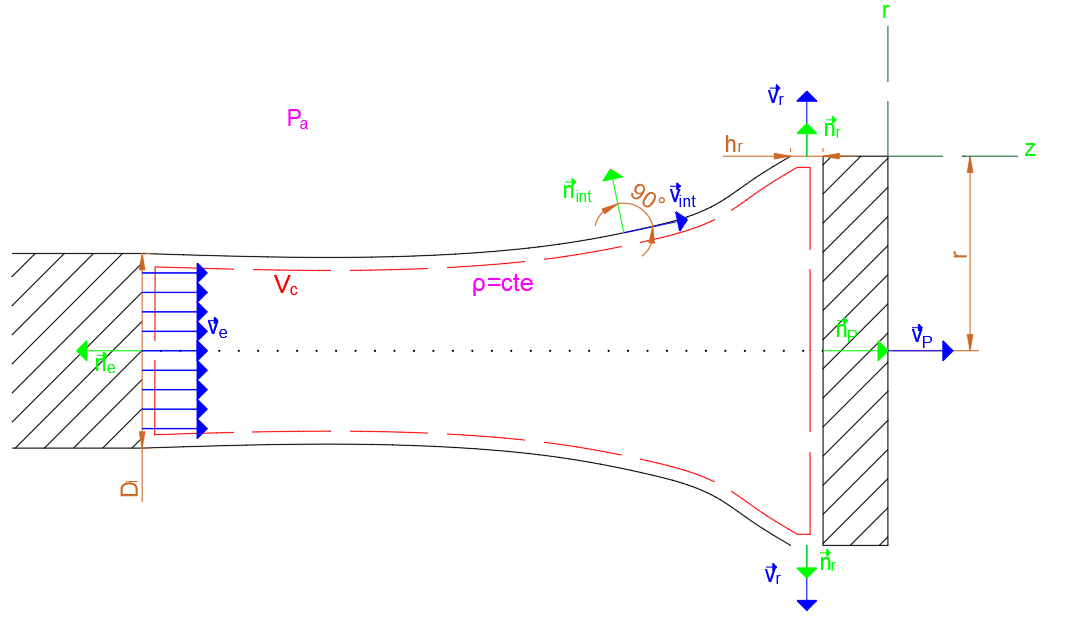
\includegraphics[width=0.7\linewidth]{imagenesEjercicios/chorro placa}
	\caption{Esquema del problema.}
	\label{fig:depositobloqueado}
\end{figure}
\textcolor{blue}
{
	Se coloca el sistema de referencia en la placa y con velocidad $\vec{v}_p$ que como es constante no provoca fuerzas de inercia. De esta manera el chorro sale a la velocidad: $\vec{v}_e-\vec{v}_p$
	\\
	Se plantea la ecuación de conservación de la masa: 
	\[\dfrac{d}{dt}\iiint_{V_c}\rho\,dV+\oiint_{S_c} \rho\left[(\vec{v}-\vec{v}_c)\cdot\vec{n}\right] \,dS=0\]
	Como el volumen de control no cambia:
	\[\dfrac{d}{dt}\iiint_{V_c}\rho\,dV=0\]
	Desarrollando el término de superficie:
	\[\oiint_{S_c} \rho\left[(\vec{v}-\vec{v}_c)\cdot\vec{n}\right] \,dS=\]
	\[
	\iint_{S_e} \rho\left[(\vec{v}-\vec{v}_c)\cdot\vec{n}\right] \,dS
	+
	\iint_{S_{int}} \rho\left[(\vec{v}-\vec{v}_c)\cdot\vec{n}\right] \,dS
	+
	\iint_{S_r} \rho\left[(\vec{v}-\vec{v}_c)\cdot\vec{n}\right] \,dS
	+
	\iint_{S_P} \rho\left[(\vec{v}-\vec{v}_c)\cdot\vec{n}\right] \,dS
	\]
	La velocidad del volumen de control $\vec{v}_c=0$
	\begin{itemize}
		\item En la salida del chorro, por ser un perfil uniforme:
			\[\iint_{S_e} \rho\left[(\vec{v}-\vec{v}_c)\cdot\vec{n}\right] \,dS=
			\iint_{S_e} \rho \left( v_e-v_P \right)\vec{i}\cdot-\vec{i} \,dS=
			-\left(v_e-v_P\right)\dfrac{\pi D^2_i}{4}\]
		\item En la interfase como la velocidad es siempre perpendicular a la superficie:
			\[\iint_{S_{int}}\rho\left[(\vec{v}-\vec{v}_c)\cdot\vec{n}\right]\,dS=0\]
		\item En la dirección radial de la placa:
			\[\iint_{S_r} \rho\left[(\vec{v}-\vec{v}_c)\cdot\vec{n}\right] \,dS=\iint_{S_r} \rho v_r\vec{e}_r\cdot\vec{e}_r \,dS=v_r2\pi r h(r) \text{[Área de un cilindro]}\]
		\item En la placa, como la velocidad del fluido es 0:
			\[\iint_{S_P} \rho\left[(\vec{v}-\vec{v}_c)\cdot\vec{n}\right]\,dS=0\]
	\end{itemize}
	Por tanto:
		\[\left(v_e-v_P\right)\dfrac{\pi D^2_i}{4}=v_r2\pi r h(r)\]
	Planteando la conservación de la cantidad de movimiento:
		\[\iiint_{V_c}\vec{f}_V\,dV
		+
		\oiint_{S_c}\left(-P\overline{\overline{I}}+\overline{\overline{\tau}}\right)\cdot\vec{n}\,dS=
		\iiint_{V_c}\dfrac{\partial \rho\vec{v}}{\partial t}\,dV
		+ \oiint_{S_c}\rho\vec{v}\left[\left(\vec{v}-\vec{v}_c\right)\cdot\vec{n}\right]\,dS\]
	Se desprecia el término de fuerzas volumétricas (número de Froude elevado):
		\[\iiint_{V_c}\vec{f}_V\,dV=0\]
	El término de fuerzas superficiales:
		\[\oiint_{S_c}\left(-P\overline{\overline{I}}+\overline{\overline{\tau}}\right)\cdot\vec{n}\,dS=\]
		\[
		\iint_{S_e}\left(-P\overline{\overline{I}}+\overline{\overline{\tau}}\right)\cdot\vec{n}\,dS
		+
		\iint_{S_{int}}\left(-P\overline{\overline{I}}+\overline{\overline{\tau}}\right)\cdot\vec{n}\,dS
		+
		\iint_{S_r}\left(-P\overline{\overline{I}}+\overline{\overline{\tau}}\right)\cdot\vec{n}\,dS
		+
		\iint_{S_P}\left(-P\overline{\overline{I}}+\overline{\overline{\tau}}\right)\cdot\vec{n}\,dS
		\]
	Aplicando el mismo razonamiento que en anteriores ejercicios se introduce la presión atmosférica $P_a$. Como el número de Reynolds y Froude son elevados porque es un líquido está dentro de un gas, $\overline{\overline{\tau}} $ es despreciable.
	\begin{itemize}
		\item En la salida del chorro, por ser un perfil uniforme y la presión es la atmosférica:
			\[\iint_{S_e}\left[-(P-P_a)\overline{\overline{I}}+\overline{\overline{\tau}}\right]\cdot\vec{n}\,dS=0\]
		\item En la interfase como la presión es la atmosférica:
			\[\iint_{S_{int}}\left[-(P-P_a)\overline{\overline{I}}+\overline{\overline{\tau}}\right]\cdot\vec{n}\,dS=0\]
		\item En la dirección radial de la placa como la presión es la atmosférica:
			\[\iint_{S_r}\left[-(P-P_a)\overline{\overline{I}}+\overline{\overline{\tau}}\right]\cdot\vec{n}\,dS=0\]
		\item En la placa:
			\[\iint_{S_p}\left[-(P-P_a)\overline{\overline{I}}+\overline{\overline{\tau}}\right]\cdot\vec{n}\,dS=-F_{jet+atm\rightarrow placa}\]
	\end{itemize}
	El término local es despreciable ya que el fluido es globalmente estacionario:
		\[\iiint_{V_c}\dfrac{\partial \rho\vec{v}}{\partial t}\,dV=0\]
	El término superficial, teniendo en cuenta como en los desarrollos anteriores solo eran no nulos los términos a la salida del chorro y en la dirección radial de la placa:
		\[\oiint_{S_c}\rho\vec{v}\left[\left(\vec{v}-\vec{v}_c\right)\cdot\vec{n}\right]\,dS=
		\iint_{S_e}\rho\vec{v}\left[\left(\vec{v}-\vec{v}_c\right)\cdot\vec{n}\right]\,dS
		+
		\iint_{S_r}\rho\vec{v}\left[\left(\vec{v}-\vec{v}_c\right)\cdot\vec{n}\right]\,dS\]
	\begin{itemize}
		\item En la salida del chorro:
			\[\iint_{S_e}\rho\vec{v}\left[\left(\vec{v}-\vec{v}_c\right)\cdot\vec{n}\right]\,dS=
			\iint_{S_e}\rho \left(v_e-v_p\right) \vec{k}\left[\left(v_e-v_p\right) \vec{k}\cdot-\vec{k}\right]\,dS=-\rho\left(v_e-v_p\right)^2\dfrac{\pi D^2_i}{4}\vec{k}\]
		\item En la dirección radial de la placa:
			\[\iint_{S_r}\rho\vec{v}\left[\left(\vec{v}-\vec{v}_c\right)\cdot\vec{n}\right]\,dS=
			\iint_{S_r}\rho v_r \vec{e}_r\left[v_r \vec{e}_r\cdot\vec{e}_r\right]\,dS=\rho v^2_r\iint_{S_r}\vec{e}_r\,dS=0 \text{ Ver figura inferior}\]
		\begin{figure}[H]
			\centering
			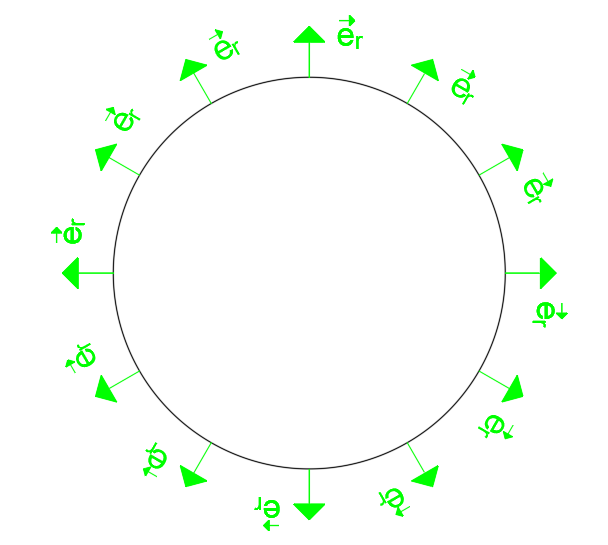
\includegraphics[width=0.6\linewidth]{imagenesEjercicios/resultante0}
			\caption{Representación de $\vec{e}_r$ a lo largo de la superficie.}
			\label{fig:resultante0}
		\end{figure}
	\end{itemize}
	Por tanto:
		\[F_{jet+atm\rightarrow placa}=\rho\left(v_e-v_p\right)^2\dfrac{\pi D^2_i}{4}\vec{k}\]
}

\newpage
\item Dado el depósito de la Figura \ref{fig:depositoaltura}, determinar la expresión de la longitud que recorre el chorro que sale del depósito, en función del tiempo.
\begin{figure}[H]
	\centering
	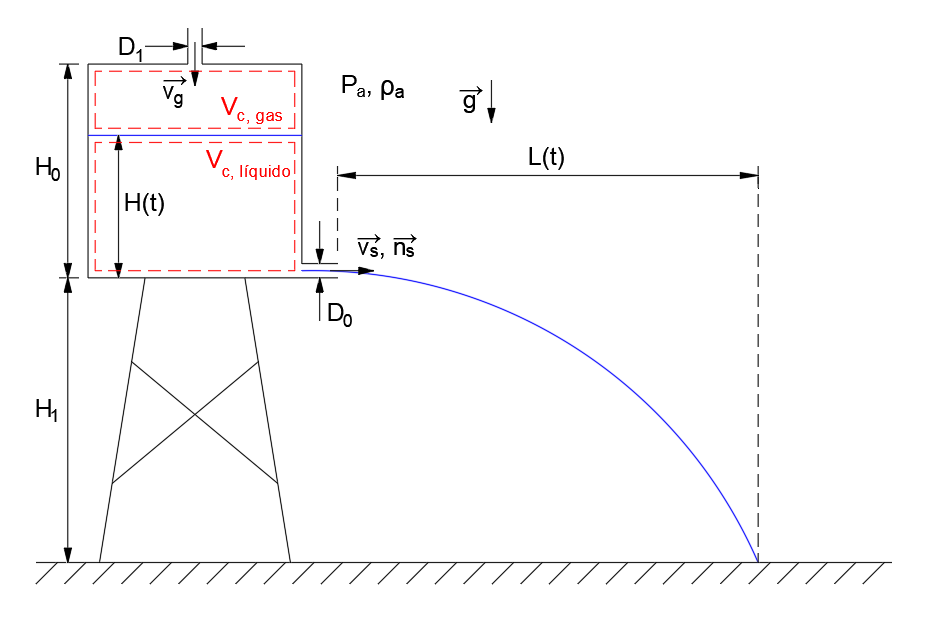
\includegraphics[width=0.9\linewidth]{imagenesEjercicios/depositoAltura}
	\caption{Esquema del depósito en altura.}
	\label{fig:depositoaltura}
\end{figure}

\blue
\textit{\textbf{Forma macroscópica.}}
\[V_C = V_{\text{depósito}} = V_{C, \text{líquido}} + V_{C, \text{gas}}\]
\[\dfrac{d}{dt} \iiint_{V_{C_l}} \rho\,dV + \oiint_{S_{C_l} = S_p \cup S_{nivel} \cup S_{salida}} \rho (\vec{v}-\vec{v}_C) \cdot \vec{n}\,dS=0\]

\begin{itemize}
	\item El término local:
	\[\dfrac{d}{dt} \iiint_{V_{C_l}} \rho\,dV = \rho A \dfrac{dH}{dt}\]
	\item El término convectivo:
	\[\oiint_{S_{C_l} = S_p \cup S_{nivel} \cup S_{salida}} \rho (\vec{v}-\vec{v}_C) \cdot \vec{n}\,dS=\rho v_s \dfrac{\pi D_0^2}{4}\]
\end{itemize}

\[-A\dfrac{dH}{dt} = v_s\dfrac{\pi D_0^2}{4}\]

\[Q_{\text{líquido}} = Q_{\text{gas}} \Rightarrow v_s\dfrac{\pi D_0^2}{4} = v_g\dfrac{\pi D_1^2}{4}\]
\[\dfrac{dV_C}{dt} = 0 \Rightarrow \dfrac{dV_{C_{\text{líquido}}}}{dt} = -\dfrac{dV_{C_{\text{gas}}}}{dt}\]

Analizando el lazo de presiones:

\[
	\begin{matrix}
		P_1 = P_a\\
		P_2 + \dfrac{1}{2}\rho_a v_g^2 = P_1 + \dfrac{1}{2}\rho_a v_{g,atm}^2\\
		P_3 = P_2(\rho_a \text{ es muy pequeña})\\
		P_4 = P_3 (\text{interfase plana})\\
		P_5 = P_4 + \rho_l g H(t)\\
		P_6 = 
		P_7 + \dfrac{1}{2} \rho_l v_s^2 = P_5\\
		P_7 = P_a
	\end{matrix}
\]

Donde $P_1$ es la presión antes del orificio 1 (por donde entra el gas), $P_2$ la presión después del orificio, $P_3$ antes de la interfase, $P_4$ después de la interfase, $P_5$ en el fondo del depósito, $P_6$ algo antes del orificio de salida y $P_7$ la presión tras salir del edificio.


Sabiendo que el término $\dfrac{1}{2}\rho_a v_{g,atm}^2$ es despreciable frente a $\dfrac{1}{2}\rho_a v_{g}^2$, tras sumar todas las presiones resulta:
\[\dfrac{1}{2}\rho_a v_{g}^2 = \dfrac{1}{2}\rho_l v_{s}^2 + \rho g H(t)\]

Conocemos las expresiones de las velocidades de entrada y salida:
\[v_g = \dfrac{Q}{\dfrac{\pi D_1^2}{4}}; v_s = \dfrac{Q}{\dfrac{\pi D_0^2}{4}}; Q = Q_g = Q_s\]

Sustituyendo en la ecuación anterior:
\[\rho_l g H(t) = \dfrac{1}{2} \rho_a \dfrac{Q^2}{\dfrac{\pi^2 D_1^4}{16}} + \dfrac{1}{2}\rho_l \dfrac{Q^2}{\dfrac{\pi^2 D_0^4}{16}} =
\dfrac{\rho_l 8 Q^2}{\pi^2 D_0^4}\left(\dfrac{\rho_a D_0^4}{\rho_l D_1^4} + 1\right) \Rightarrow\]
\[
	\begin{matrix}
		\rho_l g H(t)=\dfrac{\rho_l 8 Q^2}{\pi^2 D_0^4}\left(\dfrac{\rho_a D_0^4}{\rho_l D_1^4} + 1\right)\text{, donde }\dfrac{\rho_a D_0^4}{\rho_l D_1^4}\text{ puede llegar a ser de orden 1.}\\
		Q=-A\dfrac{dH}{dt}
	\end{matrix}
	\Biggr\} \Rightarrow\]
\[\Rightarrow Q = \sqrt{\dfrac{\pi^2 D_0^4 g}{\left(\dfrac{\rho_a D_0^4}{\rho_l D_1^4} + 1\right)} H(t)} = -A\dfrac{dH}{dt}\]

Conociendo la expresión de la caída libre:
\[\Gamma(t) = L(t)\cdot\vec{i} + Y(t)\cdot\vec{j} = t\cdot v_s(t) \cdot\vec{i} + (H_1 -\dfrac{1}{2}gt^2 )\cdot\vec{j}\]

Y despreciando la componente $\vec{j}$, despejamos la expresión pedida:
\[L(t) = 4t
\sqrt
{
	\dfrac
	{gH(t)}
	{
		\left(
		\dfrac
			{\rho_a D_0^4}
			{\rho_l D_1^4}
	 	+ 1
		\right)
	}
}
\]

\textit{\textbf{Forma microscópica.}}
	Se trata de centrarse en la interfase. No se estudiará en profundidad.
	\[\begin{matrix}
		v_l(\text{interfase}) = v_g(\text{interfase})\\
		A_l = A_g
	\end{matrix}
	\Biggr\} \Rightarrow Q_g = Q_l
	\]
	

\black
\item El movimiento de un flujo incompresible e isótropo viene dado por el campo de velocidades
$\vec{v} = (z^2 - x^2) \vec{i} + 2xz\vec{k}$. Dicho flujo se encuentra sometido a la acción de la gravedad, que actúa en la dirección negativa del eje Y. Se pide:
\begin{enumerate}
	\item Clasificar el flujo.\\
	\blue Estacionario, tridimensional, bidireccional.\\
	\black
	\item Comprobar que se verifica la ecuación de continuidad.\\
	\blue
		\[\dfrac{\partial \rho}{\partial t} + \vec{\nabla}(\rho \vec{v}) = 0\]
		\[\text{Incompresible}\Rightarrow \rho = cte \Rightarrow \dfrac{\partial \rho}{\partial t} = 0; \vec{\nabla} \cdot \vec{v} = 0\]
		
		\[
			\begin{matrix}
				\vec{\nabla} = 
					\dfrac{\partial}{\partial x} \vec{i} +
					\dfrac{\partial}{\partial y} \vec{j} +
					\dfrac{\partial}{\partial z} \vec{k}\\
				\vec{v} = v_x \vec{i} + v_y \vec{j} + v_z \vec{k}
			\end{matrix}
			\Biggr\} \Rightarrow
			\vec{\nabla}\cdot\vec{v} = 
				\dfrac{\partial v_x}{\partial x} + 
				\dfrac{\partial v_y}{\partial y} + 
				\dfrac{\partial v_z}{\partial z}	
			\Rightarrow
		\]
		
		\[\Rightarrow -2x+0+2x = 0 \Rightarrow \text{Se verifica}\]
		
	\black
	\item Calcular el campo de presiones que actúa sobre el fluido, sabiendo que la presión en el plano XZ con $y=0$ es la presión atmosférica.
	\blue
		\[
			\rho \dfrac{\partial \vec{v}}{\partial t} + \rho (\vec{v} \cdot \vec{\nabla}) \cdot \vec{v} =
				- \vec{\nabla} P + \mu \vec{\nabla}^2 \vec{v} + \rho \vec{g}
		\]
		
		Desarrollando cada término:
		
		\[\dfrac{\partial \vec{v}}{\partial t} = 0 \text{ al ser un flujo estacionario.}\]
		$(\vec{i})\,\,\,2x^3 + 2xz^2 = -\dfrac{\partial P}{\partial x}$\\
		$(\vec{j})\,\,\,0 = -\dfrac{\partial P}{\partial y} - \rho g$\\
		$(\vec{k})\,\,\,(z^2 - x^2)(2z) + 2xz(2x) = 2z^3 + 2x^2z = -\dfrac{\partial P}{\partial z}$\\
		
		$\dfrac{\partial P}{\partial x} = -2x^3 -2xz^2 \Rightarrow \int_x \Rightarrow P(x,y,z) = -\dfrac{1}{2} x^4 - x^2z^2 + f(y,z)$\\
		$\dfrac{\partial P}{\partial y} = -\rho g \Rightarrow \int_y \Rightarrow P(x,y,z) = -\rho g y + m(x,z)$\\
		$\dfrac{\partial P}{\partial z} = -2z^3 -2zx^2 \Rightarrow \int_z \Rightarrow P(x,y,z) = -\dfrac{1}{2} z^4 - z^2x^2 + h(x,y)$\\
		
		$P_a = P(x, y=0, z) = -\dfrac{1}{2} x^4 - x^2z^2 + f(y = 0,z)$\\
		$P_a = m(x,z)$\\
		$P_a = P(x, y=0, z) = -\dfrac{1}{2} z^4 - z^2x^2 + h(x,y=0)$
		
		\[\rho (\vec{v} \cdot \vec{\nabla}) \cdot \vec{v} = \rho ((z^2 - x^2)(2z-2x) + (2xz)(2z + 2x))\]
		
		$\vec{v} \cdot \vec{\nabla} = 
			v_x \dfrac{\partial}{\partial x} + 
			v_y \dfrac{\partial}{\partial y} + 
			v_z \dfrac{\partial}{\partial z}
		$\\
		
		$(\vec{v} \cdot \vec{\nabla})v_x = 
			v_x \dfrac{\partial v_x}{\partial x} + 
			v_y \dfrac{\partial v_x}{\partial y} + 
			v_z \dfrac{\partial v_x}{\partial z} =
			(z^2 - x^2)(-2x) + (2xz)(2z)
		$\\
		
		$(\vec{v} \cdot \vec{\nabla})v_y = 
			v_x \dfrac{\partial v_y}{\partial x} + 
			v_y \dfrac{\partial v_y}{\partial y} + 
			v_z \dfrac{\partial v_y}{\partial z} =
			0
		$\\
		
		$(\vec{v} \cdot \vec{\nabla})v_z = 
			v_x \dfrac{\partial v_z}{\partial x} + 
			v_y \dfrac{\partial v_z}{\partial y} + 
			v_z \dfrac{\partial v_z}{\partial z} =
			(z^2 - x^2)(2z) + (2xz)(2x)
		$
		
		\[-\vec{\nabla} P = -\left(
			\dfrac{\partial P}{\partial x} \vec{i} +
			\dfrac{\partial P}{\partial y} \vec{j} +
			\dfrac{\partial P}{\partial z} \vec{k}
			\right)
		\]	
		
		\[
			\mu \vec{\nabla}^2 \vec{v} =
				\mu \vec{\nabla}^2 v_x \vec{i} + 
				\mu \vec{\nabla}^2 v_y \vec{j} + 
				\mu \vec{\nabla}^2 v_z \vec{k} =
				\vec{0} \text{ (ver debajo)}
		\]
		
		$\vec{\nabla}^2 = \vec{\nabla} \cdot \vec{\nabla} = 
			\dfrac{\partial^2}{\partial x^2} \vec{i} +
			\dfrac{\partial^2}{\partial y^2} \vec{j} +
			\dfrac{\partial^2}{\partial z^2} \vec{k}
		$\\
		
		$\vec{\nabla}^2 v_x = -2 + 0 + 2 = 0$\\
		$\vec{\nabla}^2 v_y = 0$\\
		$\vec{\nabla}^2 v_z = 0 + 0 + 0 = 0$
		
		\[\rho \vec{g} = \vec{f}_v = -\rho g \vec{j}\]
		
\end{enumerate}


\black
\newpage
\item Para el depósito de la Figura \ref{fig:depositoAnillo} hallar la expresión del tiempo que tardaría en vaciarse sabiendo que $h(t = 0) = H_0$

\begin{figure}[H]
	\centering
	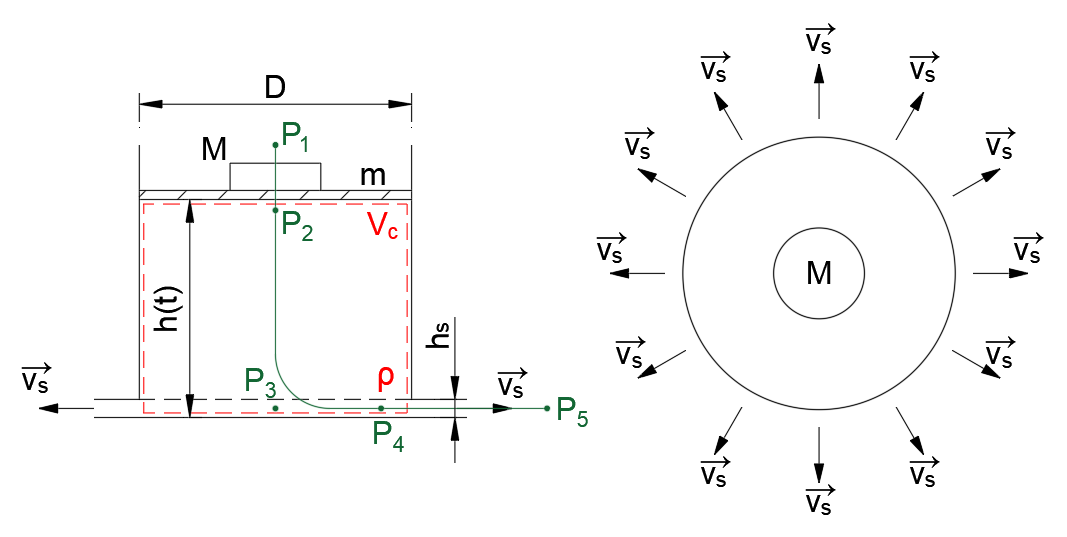
\includegraphics[width=1\linewidth]{imagenesEjercicios/depositoAnillo}
	\caption{Esquema del depósito con salida de tipo anillo.}
	\label{fig:depositoAnillo}
\end{figure}

\blue
	\textit{Conservación de la masa:}
		\[-A_d \dfrac{dh(t)}{dt} = v_s h_s \sqrt{4\pi A_d}\]
		$A_d = \dfrac{\pi D^2}{4} \Rightarrow D = \sqrt{4\pi A_d}$\\
		$P_1 = P_a$\\
		$P_2 = P_1 + (M + m)g \cdot \dfrac{1}{A_d}$\\
		$P_3 = P_2 + \rho g h(t)$\\
		$P_4 = P_3$\\
		$P_5 + \dfrac{1}{2}\rho v_s^2 = P_4$\\
		$P_5 = P_a$
		
		\[\dfrac{1}{2}\rho v_s^2 = (M + m)\dfrac{g}{A_d} + \rho g h(t)\]
		\[t_{vaciado} \Rightarrow h(t = t_{vaciado}) = 0\]
		
	Se observa que no depende de la geometría del orificio de salida, sino de la velocidad de salida del fluido.
\black
\newpage
\item Calcular la altura, h, si la fuerza del fluido sobre el depósito con N agujeros es nula. La densidad $\rho$ es constante.
\begin{figure}[H]
	\centering
	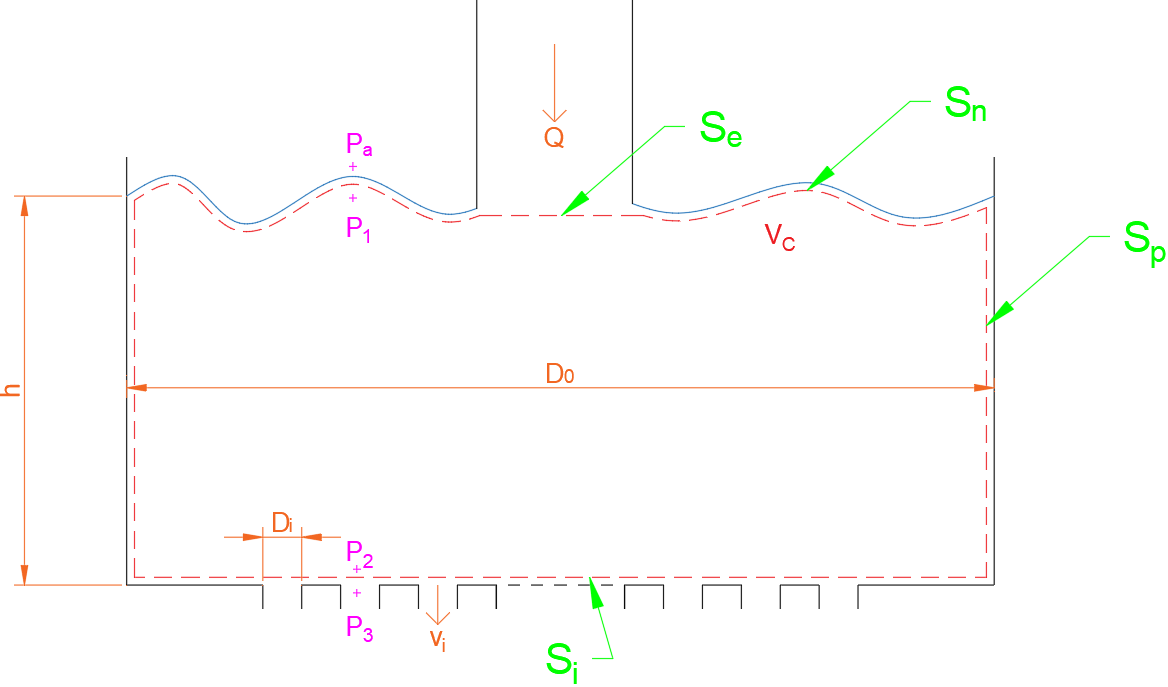
\includegraphics[width=0.6\linewidth]{imagenesEjercicios/fuerzaDepositoNagujeros}
	\caption{Esquema del depósito con N agujeros en su base.}
	\label{fig:fuerzadepositonagujeros}
\end{figure}
\blue
 Planteando la ecuación de conservación de la masa:
 \[\dfrac{d}{dt}\iiint_{V_c}\rho \,dV+\oiint_{S_c}\rho\left(\vec{v}-\vec{v}_C\right)\cdot \vec{n} \,dS=0\]
 
 
 
 Como el volumen de control no varia (h constante), teniendo en cuenta desarrollos anteriores:
 \[\dfrac{d}{dt}\iiint_{V_c}\rho \,dV=0\rightarrow \oiint_{S_c}\rho\left(\vec{v}-\vec{v}_C\right)\cdot \vec{n} \,dS=0\rightarrow \rho v_e S_e=\rho v_i S_i \rightarrow Q= v_i N\pi\dfrac{D_i^2}{4} \rightarrow v_i=\dfrac{4Q}{\pi N D_i^2}\]



	Planteando la conservación del momento en la dirección del eje $\vec{j}$ (en el eje $\vec{i}$ por simetría se anula):
	\[\left[\iiint_{V_c}\vec{f}_V\,dV
	+
	\oiint_{S_c}\left(-P\overline{\overline{I}}+\overline{\overline{\tau}}\right)\cdot\vec{n}\,dS=
	\iiint_{V_c}\dfrac{\partial \rho\vec{v}}{\partial t}\,dV
	+ \oiint_{S_c}\rho\vec{v}\left[\left(\vec{v}-\vec{v}_c\right)\cdot\vec{n}\right]\,dS\right]\cdot \vec{j}\]
	El término de fuerzas volumétricas:
	\[\iiint_{V_c}\vec{f}_V\,dV \cdot \vec{j}=-\rho g h A_d\]
	El término de fuerzas superficiales:
	\[\oiint_{S_c}\left(-P\overline{\overline{I}}+\overline{\overline{\tau}}\right)\cdot\vec{n}\,dS=\]
	\[
	\iint_{S_e}\left(-P\overline{\overline{I}}+\overline{\overline{\tau}}\right)\cdot\vec{n}\,dS
	+
	\iint_{S_{i}}\left(-P\overline{\overline{I}}+\overline{\overline{\tau}}\right)\cdot\vec{n}\,dS
	+
	\iint_{S_n}\left(-P\overline{\overline{I}}+\overline{\overline{\tau}}\right)\cdot\vec{n}\,dS
	+
	\iint_{S_p}\left(-P\overline{\overline{I}}+\overline{\overline{\tau}}\right)\cdot\vec{n}\,dS
	\]
	Aplicando el mismo razonamiento que en anteriores ejercicios se introduce la presión atmosférica $P_a$. Como el número de Reynolds es elevado, $\overline{\overline{\tau}} $ es despreciable. 
	\begin{itemize}
		\item En la entrada del chorro, por ser un perfil uniforme y la presión es la atmosférica:
		\[\left\{\iint_{S_e}\left[-(P-P_a)\overline{\overline{I}}+\overline{\overline{\tau}}\right]\cdot\vec{n}\,dS\right\}\cdot \vec{j}=0\]
		\item En la salida del chorro, por ser un perfil uniforme y la presión es la atmosférica:
		\[\left\{\iint_{S_{i}}\left[-(P-P_a)\overline{\overline{I}}+\overline{\overline{\tau}}\right]\cdot\vec{n}\,dS\right\}\cdot \vec{j}=0\]
		\item En interfase líquido-gas como la presión es la atmosférica:
		\[\left\{\iint_{S_n}\left[-(P-P_a)\overline{\overline{I}}+\overline{\overline{\tau}}\right]\cdot\vec{n}\,dS\right\}\cdot \vec{j}=0\]
		\item En la pared:
		\[\left\{\iint_{S_p}\left[-(P-P_a)\overline{\overline{I}}+\overline{\overline{\tau}}\right]\cdot\vec{n}\,dS\right\}\cdot \vec{j}=-F_{liq+atm\rightarrow placa}\]
	\end{itemize}
	El término local es nulo, pues h es constante:
	\[\iiint_{V_c}\dfrac{\partial \rho\vec{v}}{\partial t}\,dV=0\]
	El término superficial, teniendo en cuenta que salvo en la salida y en la entrada los términos son nulos:
	\[\left[\oiint_{S_c}\rho\vec{v}\left[\left(\vec{v}-\vec{v}_c\right)\cdot\vec{n}\right]\,dS=
	\iint_{S_e}\rho\vec{v}\left[\left(\vec{v}-\vec{v}_c\right)\cdot\vec{n}\right]\,dS
	+
	\iint_{S_i}\rho\vec{v}\left[\left(\vec{v}-\vec{v}_c\right)\cdot\vec{n}\right]\,dS\right]\cdot\vec{j}\]
	\begin{itemize}
		\item En la entrada del chorro:
		\[\left[\iint_{S_e}\rho\vec{v}\left[\left(\vec{v}-\vec{v}_c\right)\cdot\vec{n}\right]\,dS\right]\cdot \vec{j}=
		\left[\iint_{S_e}\rho v_e\vec{j}\left[v_e \vec{j}\cdot-\vec{j}\right]\,dS\right]\vec{j}=-\rho \dfrac{4Q^2}{\pi D_0^2}\]
		\item En la salida del chorro:
		\[\left[\iint_{S_i}\rho\vec{v}\left[\left(\vec{v}-\vec{v}_c\right)\cdot\vec{n}\right]\,dS\right]\cdot \vec{j}=
		\left[\iint_{S_i}-\rho v_i\vec{j}\left[-v_i \vec{j}\cdot-\vec{j}\right]\,dS\right]\vec{j}=-\rho N v_i^2\dfrac{D_i^2\pi}{4}
		 \]
	\end{itemize}
	Por tanto:
	\[-\rho g h A_d-F_{jet+atm\rightarrow placa}=-\rho \dfrac{4Q^2}{\pi D_0^2}-\rho N v_i^2\dfrac{D_i^2\pi}{4}\]
	\[F_{jet+atm\rightarrow placa}=\rho\left(\dfrac{4Q^2}{\pi D_0^2}+ N v_i^2\dfrac{D_i^2\pi}{4}- g h A_d\right)=0\]
	\[\dfrac{4Q^2}{\pi D_0^2}+ N v_i^2\dfrac{D_i^2\pi}{4}- g h A_d=0\]
	
	
	
	Sustituyendo la expresión obtenida mediante conservación de la masa:
	\[N^2v_i^2\dfrac{\pi  D_i^4}{4 D_0^2}+ N v_i^2\dfrac{\pi D_i^2}{4}- g h \dfrac{\pi D_0^2}{4}=0\rightarrow
	 gh=v_i^2\left[\left(\dfrac{ \sqrt{N} D_i}{D_0}\right)^4+ \left(\dfrac{ \sqrt{N} D_i}{D_0}\right)^2\right]\]
	 
	 
	 Mediante el lazo de presiones se puede obtener otra relación entre altura y velocidad:
	 \[P_a=P_1\]
	 \[P_1+\rho g h=P_2\]
	 \[P_2=P_3+\dfrac{\rho v_i^2}{2}\]
	 \[P_3=P_a\]
	 \[g h=\dfrac{v_i^2}{2}\]
	 
	 
	 Por tanto, para que la altura sea constante debe cumplirse que (tanto la ecuación por lazo de presiones como mediante conservación de la masa deben ser iguales):
	 \[\dfrac{1}{2}=\left(\dfrac{ \sqrt{N} D_i}{D_0}\right)^4+ \left(\dfrac{ \sqrt{N} D_i}{D_0}\right)^2\]
	 
	 
	 Cuya única solución real positiva es:
	 \[\dfrac{ \sqrt{N} D_i}{D_0}=\sqrt{\dfrac{\sqrt{3}}{2}-\dfrac{1}{2}}\approx 0,605 \rightarrow \sqrt{N} D_i\approx0,605 D_0\]
\black

%Dibujo realizado, pero falta solución
%\item Hallar la expresión de la presión a aplicar sobre la masa en función de las magnitudes del problema. Tomar que R$<<$H.
%
%	\begin{figure}[H]
%	\begin{minipage}{0.6\textwidth}
%		\centering
%		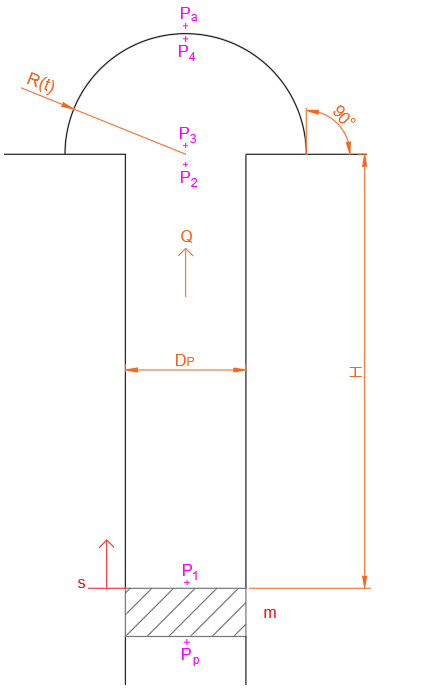
\includegraphics[width=0.7\linewidth]{imagenesEjercicios/masaMovilRadio}
%		\caption{Esquema del problema.}
%		\label{fig:masamovilradio}
%	\end{minipage}%
%	\begin{minipage}{0.4\textwidth}
%	\blue	
%	\end{minipage}
%\end{figure}

\end{enumerate}
\black
\section{Flujos de viscosidad dominante.}
\begin{enumerate}
	\item Hallar la velocidad mínima para arrastrar toda la película líquida hacia arriba. $\mu$ y $\rho$ constantes.
	\begin{figure}[H]
		\begin{minipage}{0.45\textwidth}
		\centering
		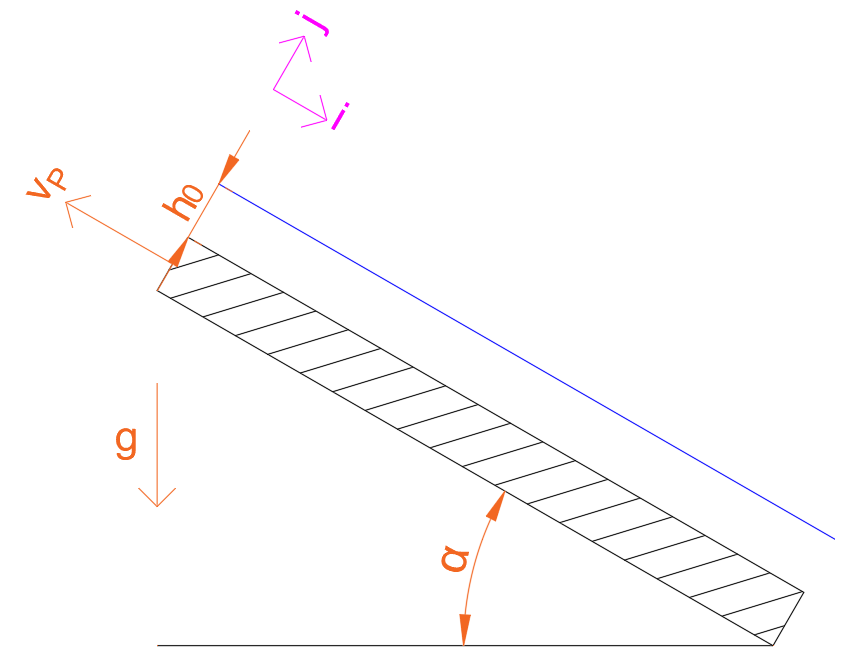
\includegraphics[width=0.8\linewidth]{imagenesEjercicios/arrastreFluido}
		\caption{Esquema de la placa arrastrando el fluido.}
		\label{fig:arrastrefluido}
	\end{minipage}%
	\begin{minipage}{0.55\textwidth}
	\blue
	Planteando las ecuaciones vistas en el tema para un flujo con fuerzas de viscosidad dominante unidireccional:
	\[0=P_l+\mu\dfrac{\partial v_x^2}{\partial^2 y}\ \ ; \ \ P_l=-\dfrac{\partial }{\partial x}\left(P+\rho U \right)\]
	
	Las condiciones de contorno del problema son:
	\[v_x(y=0)=-v_p \ \ ; \ \ P(y=h_0)=P_a\]
	\[ \tau_{P_{l}}=\mu_{liq} \left. \dfrac{\partial v_x}{\partial y} \right|_{liq} =\mu_{gas} \left. \dfrac{\partial v_x}{\partial y} \right|_{gas} \approx 0\]
	\[U=U_g=-\vec{g}\cdot \vec{r}=g\vec{j'}\cdot
	\left(x\vec{i}+y\vec{j}\right)\]
	\[U= g\left(-x sen(\alpha)+ycos(\alpha)\right)\]
	\[P+\rho U=P+\rho g\left(-x sen(\alpha)+ycos(\alpha)\right)\]
	\end{minipage}
	\end{figure}
	\blue
	\[P_l=-\dfrac{\partial }{\partial x}\left(P+\rho U\right)=
	-\dfrac{\partial }{\partial x}\left[P+\rho g\left(-x sen(\alpha)+ycos(\alpha)\right)\right]=\rho gsen(\alpha)\]	
	\[0=P_l+\mu\dfrac{\partial v_x^2}{\partial^2 y}\rightarrow \dfrac{\partial v_x^2}{\partial^2 y}=-\dfrac{P_l}{\mu}\rightarrow v_x=-\dfrac{P_l}{2\mu}y^2+Ay+B\]
	\[v_x(y=0)=-v_p\rightarrow B=-v_p \ \ ; \ \ \left. \dfrac{\partial v_x}{\partial y} \right|_{h_0}=0 \rightarrow A=\dfrac{P_l}{\mu}h_0\]
	\[v_x=\dfrac{P_l y}{2\mu}\left(h_0-y\right)-v_p\]
	
	
	Para que arrastre toda la película de líquido:
	\[v_x=\dfrac{P_l y}{2\mu}\left(h_0-y\right)-v_p < 0 \ \forall \ y\]
	\black
	\item Hallar la dinámica del vaciado si el flujo es de viscosidad dominante. El fluido tiene $\mu$ y $\rho$ constantes.
	\begin{figure}[H]
		\begin{minipage}{0.45\textwidth}
			\centering
			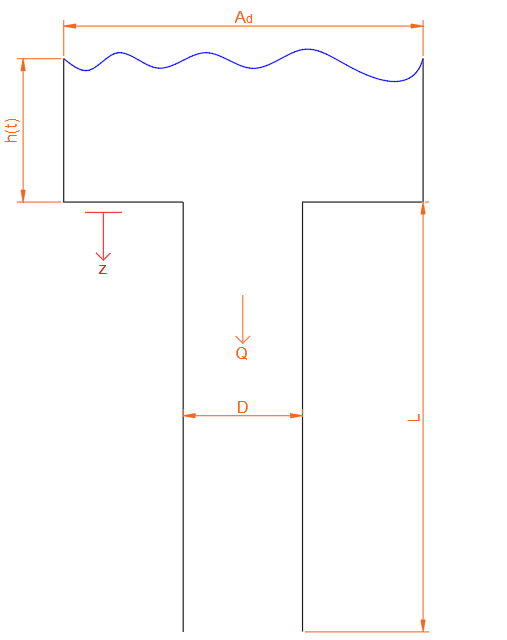
\includegraphics[width=1\linewidth]{imagenesEjercicios/flujoViscosidadDominante1}
			\caption{Esquema del depósito vaciandose.}
			\label{fig:flujoviscosidaddominante1}
		\end{minipage}%
		\begin{minipage}{0.55\textwidth}
			\blue
			Se parte de la expresión del flujo de Hagen-Poiseuille
			\[Q=-A_d \dot{h}(t) \ \ ; \ \ Q_{H-P}=-\dfrac{\pi D^4}{128 \mu}\dfrac{\partial}{\partial z}\left(P+\rho U\right)\]
			\[-\dfrac{\partial}{\partial z}\left(P+\rho U\right)=\dfrac{128 \mu Q}{\pi D^4}\rightarrow Q \ y \ D \ne f(z)\]
			\[\dfrac{\left(P+\rho  U\right)_{z=0}-\left(P+\rho  U\right)_{z=L}}{L}=\dfrac{128 \mu Q}{\pi D^4}\]
			\[\left(P+\rho  U\right)_{z=0}=\left(P+\rho  U\right)_{e}=P_e\]
			\[\left(P+\rho  U\right)_{z=0}=\left(P+\rho  U\right)_{s}=P_s-\rho g L\]
		
			
			Sustituyendo:
			\[P_e-\left(P_s-\rho g L\right)=\dfrac{128 \mu QL}{\pi D^4}\rightarrow P_e+\rho g L=P_s+\dfrac{128 \mu QL}{\pi D^4}\]
				\[P_e=P_a+\rho g h(t)\]
			\[P_s=P_a\]
			\[\rho g\left[L+h(t)\right]=\dfrac{128 \mu L}{\pi D^4}Q=-\dfrac{128 \mu L}{\pi D^4}A_d \dot{h}(t)\]
		\end{minipage}
	\end{figure}
	\blue
	Resolviendo la EDO:
	\[\dfrac{dh}{L+h(t)}=-\dfrac{\rho g\pi D^4}{128 \mu L A_d }dt
	\rightarrow
	 ln\left[L+h(t)\right]=-\dfrac{\rho g\pi D^4}{128 \mu L A_d }t +C\]
	\[h(t=0)=h_0 \rightarrow ln\left[L+h_0\right]=C\]
	
	
	Por tanto:
	\[ ln\left[\dfrac{L+h(t)}{L+h_0}\right]=-\dfrac{\rho g\pi D^4}{128 \mu L A_d }t \rightarrow K= \dfrac{\rho g\pi D^4}{128 \mu L A_d } \rightarrow h(t)=L\left(e^{-Kt}-1\right) + h_0e^{-Kt}\]
	\newpage
	\black
	\item Hallar la dinámica del sistema si el flujo de viscosidad dominante está inmerso en una tubería de diámetro descendente. $D=D_0\left(1-\alpha\dfrac{z}{L}\right)$
	\begin{figure}[H]
		\centering
		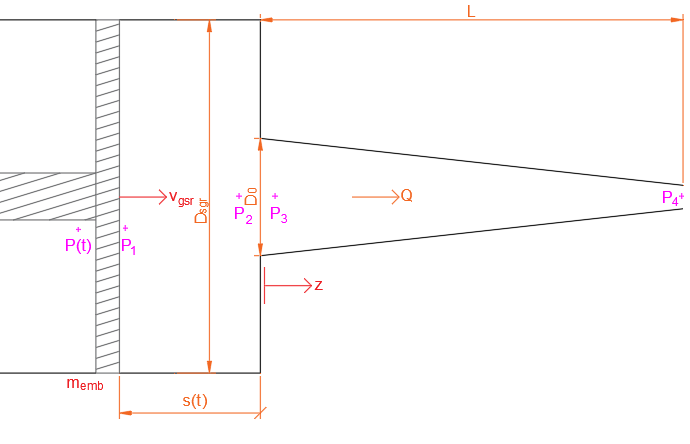
\includegraphics[width=0.8\linewidth]{imagenesEjercicios/emboloDiametroDescendente}
		\caption{Esquema del problema.}
		\label{fig:embolodiametrodescendente}
	\end{figure}
	\blue
	Sea $P(t)=At+B$. Planteando el lazo de presiones:
	\[m_{emb}\ddot{s}=\left[P(t)-P_1\right]\dfrac{\pi D_{sgr}^2}{4} \rightarrow P(t)=P_1 -\dfrac{4m_{emb}}{\pi D_{sgr}^2}\ddot{s}\]
	\[P_1=P_2=P_3\]
	\[Q_{H-P}=-\dfrac{\pi D^4(z)}{128}\dfrac{\partial}{\partial z}\left(P+\rho U\right) \rightarrow P_3-P_4 =\dfrac{128\mu Q}{\pi}\int_0^L \dfrac{1}{D^4(z)}\,dz\]
	\[P_3-P_4 =\dfrac{128\mu Q}{\pi}\int_0^L \dfrac{1}{\left(1-\alpha\dfrac{z}{L}\right)^4}\,dz=
	\left.\dfrac{128\mu Q}{\pi} \dfrac{3\alpha}{\left(1-\alpha\dfrac{z}{L}\right)^3}  \right|_0^L
	= \dfrac{384\mu Q \alpha}{\pi} \left[\dfrac{1}{\left(1-\alpha\right)^3 }- 1\right]
	\]
	
	
	Planteando las ecuaciones de conservación de la masa se obtiene:
	\[Q=-\dot{s}\dfrac{\pi D_{sgr^2}}{4}\]
	\black 
\end{enumerate}
\newpage
\black
\section{Conservación de la energía.}
\begin{enumerate}
	\item Calcular la potencia que debería tener la bomba para levantar el pistón a velocidad constante.
	\begin{figure}[H]
		\centering
		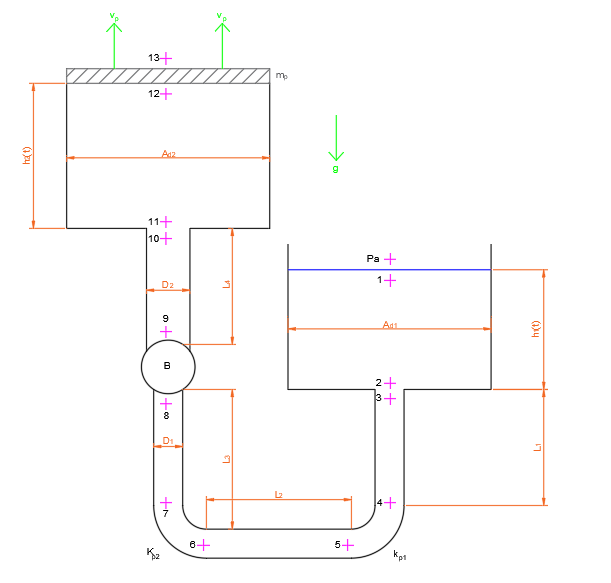
\includegraphics[width=0.7\linewidth]{imagenesEjercicios/Ej1Perdidas}
		\caption{Representación del sistema.}
		\label{fig:ej1perdidas}
	\end{figure}
	\blue
	Se consideran orificios ideales y fricción por los tubos despreciable. Por conservación de la masa el caudal es el mismo en todo el recorrido. Planteando el equilibrio de presiones:
	\[P_1=P_a\]
	\[P_2=P_1+\rho g h_1(t)\]
	\[P_3+\rho \dfrac{v_3^2}{2}=P_2\]
	\[P_4=P_3+\rho g L_1\]
	\[K_{p1}\rho\dfrac{v_4^2}{2}+P_5+\rho \dfrac{v_5^2}{2}=P_4+\rho \dfrac{v_4^2}{2} \rightarrow K_{p1}\rho\dfrac{v_4^2}{2}+P_5=P_4\]
	\[P_6=P_5\]
	\[P_7+K_{p2}\rho \dfrac{v_6^2}{2}=P_6\]
	\[P_8+\rho g L_3 =P_7\]
	\[Q\left[\left(P_9+\rho \dfrac{v_9^2}{2}\right)-\left(P_8+\rho \dfrac{v_8^2}{2}\right)\right]=\dot{W}_B\]
	\[P_9=P_{10}+\rho g L_4\]
	
	
	Cuando se produce una descarga de conducto a depósito, localmente, la energía cinética se diluye y por tanto, la presión no varia.
	\[P_{10}=P_{11}\]
	\[P_{11}=P_{12}+\rho g h_2(t)\]
	\[A_{d2}(P_{12}-P_{13})=m_p \ddot{h}_2(t)+m_p g=m_p g \rightarrow [\ddot{h}_2(t) = 0, \text{velocidad constante}]\]
	\[P_{13}=P_a\]
	
	
	Sumando todas las ecuaciones y sabiendo que mediante conservación de la masa:
	\[v_3=v_4=v_5=v_6=v_7=v_8\]
	\[v_9=v_{10}\]
	\[Q=v_8\dfrac{\pi D_1^2}{4}=v_9\dfrac{\pi D_2^2}{4} \rightarrow v_8= v_9\dfrac{D_2^2}{D_1^2}\]
	\[P_8+\rho\dfrac{v_8^2}{2}=P_a+\rho g \left[h_1(t)+L_1-L_3\right]-\rho\dfrac{v_8^2}{2}(K_{p1}+K_{p2})\]
	\[P_9=P_a+\rho g \left[L_4+h_2(t)\right]+\dfrac{m_p g}{A_d}\]
	
	
	Sustituyendo en la ecuación anteriormente obtenida para la bomba:
	\[Q\left[\left(P_a+\rho g \left[L_4+h_2(t)\right]+\dfrac{m_p g}{A_d}+\rho \dfrac{v_9^2}{2}\right)
	-\left(P_a+\rho g \left[h_1(t)+L_1-L_3\right]-\rho\dfrac{v_8^2}{2}(K_{p1}+K_{p2})\right)\right]=\dot{W}_B\]
	
	\[v_9\dfrac{\pi D_2^2}{4}\left[\left(P_a+\rho g \left[L_4+h_2(t)\right]+\dfrac{m_p g}{A_d}+\rho \dfrac{v_9^2}{2}\right)
	-\left(P_a+\rho g \left[h_1(t)+L_1-L_3\right]-\rho\dfrac{v_9^2}{2}\dfrac{D_2^2}{D_1^2}(K_{p1}+K_{p2})\right)\right]=\dot{W}_B\]
	
	
	Por último, también se cumple que:
	\[Q=-A_{d1}\dot{h}_1=A_{d2} v_p = cte\rightarrow h_1(t)=h_{01}-QA_{d1}t \rightarrow h_2(t)=h_{02}+QA_{d2}t\]
	\black
	\item Hallar la relación de presiones en el siguiente sistema.
		
	\begin{figure}[H]
		\centering
		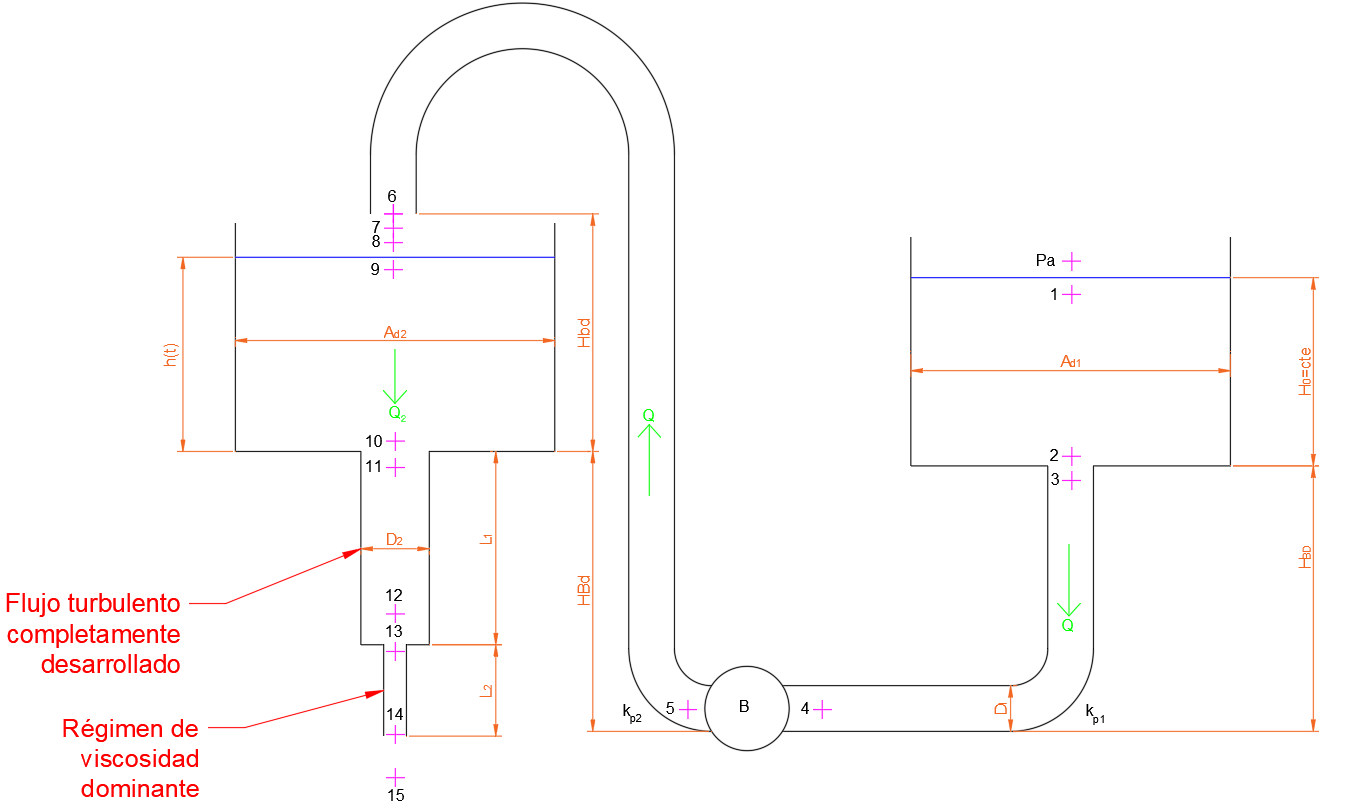
\includegraphics[width=0.8\linewidth]{imagenesEjercicios/Ej1Perdidas2}
		\caption{Representación del sistema.}
		\label{fig:ej1perdidas2}
	\end{figure}
	\blue
	El problema está dividido en dos lazos de presión. En los puntos 1-7 se estudia el sistema de bombeo y en los puntos 8-15 el sistema de abastecimiento.
	\[P_1=P_a\]
	\[P_2=P_1+\rho g H_0\]
	\[P_3+\rho \dfrac{v_3^2}{2}=P_2\]
	\[K_{p1}\rho \dfrac{v_3^2}{2} + P_4=P_3+\rho g H_{BD}\]
	\[Q(P_5-P_4)=\dot{W}_B\]
	\[K_{P2}\rho \dfrac{v_5^2}{2}+P_6+\rho g(H_{Bd}+H_{bd})=P_5\]
	\[P_6=P_7=P_8=P_9=P_a\]
	\[P_{10}=P_9+\rho g h(t)\]
	\[P_{11}+\rho\dfrac{v_{11}^2}{2}=P_{10}\]
	\[ \left(P_{11}+\rho\dfrac{v_{11}^2}{2}+\rho g z_{11}\right)-\left(P_{12}+\rho\dfrac{v_{12}^2}{2}+\rho g z_{12} \right)=f
	\dfrac{\rho v_{11}^2 L_1}{2D_2}\rightarrow v_{11}=v_{12} \rightarrow P_{11} +\rho g L_1=P_{12}+f
	\dfrac{\rho v_{11}^2 L_1}{2D_2}\]
	\[P_{13}=P_{12} \rightarrow \text{(Disipación turbulenta en viscosidad)}\]
	\[\dfrac{128\mu L_2 Q_2}{\pi D^4}=P_{13}+\rho g L_2 - P_{14}\]
	\[P_{14}=P_{15}=P_a\]
	\black
	
	
	\item Un petrolero ha llegado a puerto con una carga de petróleo crudo de densidad relativa 0,86
	y viscosidad cinemática de 5 $mm^2/s$. Esta carga se debe descargar el el depósito indicado
	para su almacenamiento. A tal fin, la instalación de descarga dispone de):
	
	\begin{enumerate}
		\item Una bomba de 20 kW cuyo rendimiento global es de 0,7
		\item Una conducción, de fundición, que tiene 25 cm de diámetro y una longitud de 200
		m en la que existen 4 codos y una válvula reguladora de caudal cuyas longitudes
		equivalentes son respectivamente, 4 m por cada codo y 24 m por la válvula.
	\end{enumerate}
	Teniendo en cuenta que $h_1 = 1 m$, $h_2 = 30 m$, que la rugosidad absoluta es 0,26 mm
	y considerando que la pérdida de carga unitaria viene dada por la expresión de Darcy-
	Weissbach, determínese el caudal de descarga.
	\begin{figure}[H]
		\centering
		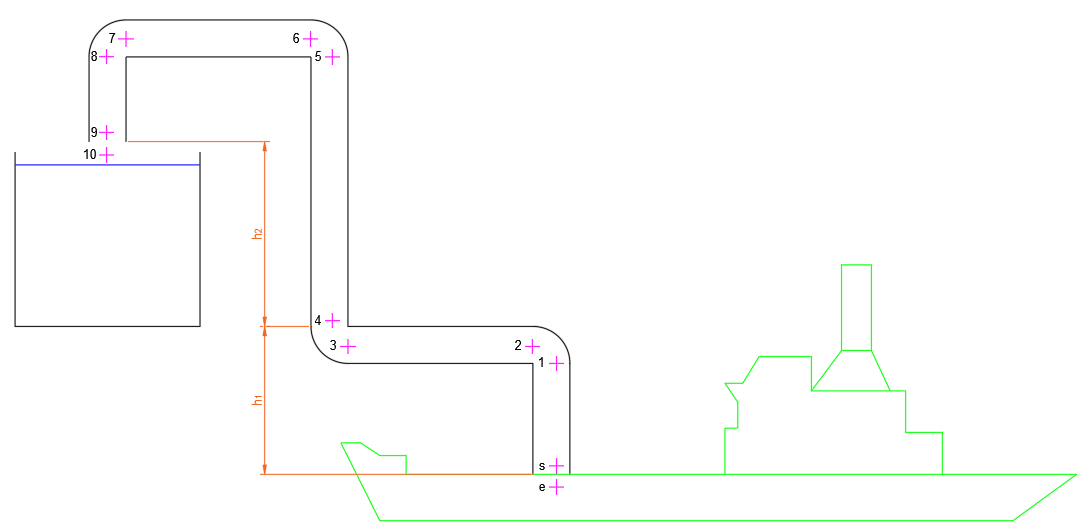
\includegraphics[width=1\linewidth]{imagenesEjercicios/Ej1Perdidas4}
		\caption{Esquema del problema.}
		\label{fig:ej1perdidas4}
	\end{figure}
	\blue
	En este ejercicio, en lugar de darse el factor K de pérdidas se da una longitud equivalente de pérdidas. De esta manera, las pérdidas serán equivalentes a las que ocurrirían en un conducto de dicha longitud. Por tanto, aunque se podrían hacer las presiones en los distintos puntos intermedios, basta con obtener las presiones en s y 9.
	\[P_e=P_a\]
	\[Q\left[\left(P_s+\dfrac{\rho v_s^2}{2}+\rho g z_{s}\right)-\left(P_e+\dfrac{\rho v_e^2}{2}+\rho g z_{e}\right)\right]=\eta \dot{W}_B\rightarrow 
	Q\left[P_s-P_e\right]=\eta \dot{W}_B \]
	\[\left(P_s+\dfrac{\rho v_s^2}{2}+\rho g z_{s}\right)-\left(P_9+\dfrac{\rho v_9^2}{2}+\rho g z_{9}\right)=
	\dfrac{\rho f v^2 L_v }{2D} \rightarrow v_s=v_9 \rightarrow
	P_s=P_9+\rho g (h_1+h_2)+\dfrac{\rho f v^2 L_v }{2D}\]
	
	
	En función del caudal, Q quedaría:
	\[v=\dfrac{4Q }{\pi D^2}\rightarrow P_s=P_9+\rho g (h_1+h_2)+\dfrac{8\rho f Q^2 L_v }{\pi^2 D^5 }\]
	\[P_9=P_{10}=P_a\]	
	
	
	Despejando Q a partir de las ecuaciones:
	\[Q\left[P_a+\rho g (h_1+h_2)+\dfrac{8\rho f Q^2 L_v }{\pi^2 D^5 }-P_a\right]=\eta \dot{W}_B\]
	\[Q^3\cdot \dfrac{8\rho fL_v }{\pi^2 D^5 }+ Q\cdot \rho g (h_1+h_2) =\eta \dot{W}_B\]
	
	
	
	A continuación, se obtienen los valores numéricos:
	\[\eta= 0.7\]
	\[\dot{W}_B=20kW\]
	\[\rho=0,86 \rho_{H_2O}=0,86\times 1000 \dfrac{kg}{m^3}=860 \dfrac{kg}{m^3}\]
	\[g=9,81\dfrac{m}{s^2}\]
	\[h_1=1m\]
	\[h_2=30m\]
	\[D=0,25 m\]
	\[L_v=200+4\cdot4+24=240m\]
	\[\epsilon=5\times 10^{-6} \dfrac{m^2}{s}\]
	
	
	Para obtener el valor de f, se emplea el ábaco de Moody. Para ello, se calcula la rugosidad relativa y se asume un Reynolds elevado (luego se comprueba).
	\[\epsilon_R=\dfrac{\epsilon}{D}=\dfrac{0,26\times10^{-3}}{0,25}=0,00104 \rightarrow \text{Se corresponde con una f de 0,02}\]
	
	
	Sustituyendo:
	\[Q^3\times 110504 + Q\times 261268=14000\rightarrow Q=0,054 \dfrac{m^3}{s}\]
	\[v=\dfrac{4Q }{\pi D^2}=\dfrac{4\times 0,054}{\pi \times 0,25^2}=1,1 \dfrac{m}{s}\]
	
	El número de Reynolds:
	\[Re=\dfrac{\rho v_c L_c}{\mu} \rightarrow L_c = D \ \ y \ \ \mu= \rho \nu\]
	\[L_c=0,25 m\]
	\[\mu = 860\times (5\times 10^{-6})=0,0043 Pa \cdot s\]
	\[Re=\dfrac{860 \times 1,1 \times 0,25}{0,0043}=55000\]


	Comprobando con el diagrama de Moody, la aproximación inicial de suponer un Reynolds elevado es válida y, por tanto, no es necesario iterar.
\end{enumerate}
\black
\newpage
\section{Fluidoestática.}
\section{Semejanza hidrodinámica.}



	
\end{document}